\documentclass{thesis}

\thesisTitle{Uncertainty quantification for surface reconstruction from partial point clouds}
\thesisType{Master Thesis}
\thesisAuthor{Debabrata Ghosh}
\thesisStudentID{441275}
\thesisMonth{June 2025}
\thesisAdvisor{Dr. Isak Lim}
\thesisPrimaryReviewer{Prof.\ Dr.\ Leif Kobbelt}
\thesisSecondaryReviewer{Prof.\ Dr.\ Kuhlen Torsten}

\begin{document}
\makeFrontMatter

\chapter*{}
\begin{center}
    \textbf{Abstract}\\
\end{center}
Point clouds of a 3D object obtained via scanning are often noisy and incomplete. It is essential to then reconstruct the underlying surface and quantify the uncertainty from the sparse data available, enabling the execution of many downstream tasks.

Existing methods have provided uncertainty quantification for reconstructed surfaces from complete scans by utilizing normal information. However, normals and complete scans are often not available in real-life applications, and only a sparse point cloud is observed. This thesis focuses on quantifying the uncertainty of surface reconstruction from a partial point cloud, either in the form of a completed point cloud or an implicit representation.

We employed different uncertainty quantification methods for deep learning in our thesis. We generated different possible completed clouds to empirically compute the average and variance of the distribution of generated clouds. For the implicit representation, we implemented the same empirical approach. Furthermore, we attempted to model the implicit function values as observations of a Gaussian process to learn a distribution over the possible implicit functions, thereby directly quantifying uncertainty without any empirical estimation.

\mainmatter
\chapter{Introduction}\label{ch:introduction}
Reconstructing curved surfaces from point clouds is a well-studied problem in the field of computer graphics, as point clouds are widely used to represent 3D shapes due to the ease of obtaining point cloud data (via scanning). It refers to the process of converting a discrete set of points in 3D space to another representation for two-dimensional manifolds, such as a mesh or an implicit function. Such an underdetermined process is inherently uncertain. Moreover, often the captured 3D geometry is noisy and sparse or incomplete due to limited sensor resolution, viewing angle, and occlusion, leading to further uncertainty. It is crucial to reconstruct the incomplete 3D shape in its entirety for a better understanding of 3D shapes or scenes, and for various downstream tasks such as simulation, next-view planning, grasping, path planning, collision detection, and so on. 

Many learning-based methods~\cite{PCN, PoinTr, PointAttN, P2C, VarPCN, PCNSkip, Snowflake} implemented point cloud completion for a given incomplete point cloud by predicting the missing points or the complete point cloud. Such a deterministic one-to-one mapping is restrictive in terms of diverse completion since one incomplete shape can be completed in many different ways, leading to various geometries. To address this issue, certain works have introduced different generative model-based strategies~\cite{HyperPocket, CGAN, PCCIMLE, EBResLT} to generate multiple complete point clouds for a given partial point cloud as input. For supervised point completion, generating multiple shapes from a single partial shape is difficult, since we only have one complete ground truth shape available for each partial input during training.~\cite{CGAN} addressed this issue by using a conditional generative adversarial network (GAN) to generate multiple complete clouds during inference. But because of mode collapse in GANs~\cite{ModeCollapseGAN}, generated shapes are often not geometrically diverse and differ only in simpler aspects such as length or width.~\cite{PCCIMLE} used implicit maximum likelihood estimation (IMLE) introduced in~\cite{IMLE} instead of GANs to incorporate multiple completions for an input partial shape without the downside of mode collapse.~\cite{HyperPocket} predicted the missing parts of the shapes rather than generating complete shapes by enforcing the representation of the missing point cloud space to follow a probability distribution and using a hypernetwork~\cite{Hypernet} to train a decoder that takes the concatenated representations of the partial and missing points and outputs weights of the target network. The target network is trained to produce a complete point cloud from a probability distribution as implemented in~\cite{PCHypernet}. ~\cite{EBResLT} proposed incorporating an energy-based model (EBM)~\cite{EBM} to transport the partial cloud representation to the complete cloud representation using residual (the difference between partial and complete representations) in an unsupervised setting. Among such methods, only~\cite{EBResLT} provided an uncertainty map for the multiple clouds generated for a partial input cloud by performing multiple inferences and naively computing the mean and variance for each point without any assumption about their correspondences, following the approach suggested in~\cite{UncertDeepL}. Following such an approach, we do not know any one-to-one mapping of individual points between the generated clouds. Also, such methods cannot restrict producing a complete cloud in a manner where each point corresponds to a particular position in the 3D shape. This might lead to completely unrelated points matched together, leading to erroneous mean and variance estimations.

To find a more meaningful matching between generated clouds, we posed this as a linear assignment problem with a suitable cost function (e.g., Euclidean distance). We fixed one generated complete cloud and found one-to-one mappings with points in the other complete clouds, and used the resulting matching to compute the mean and variance estimation of the predicted complete point cloud. This simple matching can be extended to any generative completion methods that can produce multiple possible predictions. \textit{\color{red}(Should I include the resulting differences here?)} \textbf{\color{orange} Explain how to do surface reconstruction from here to show uncertain surfaces! That should refer to the following works below, which do direct surface reconstructions!}
 
Extensive work has been done in terms of reconstructing surfaces from point clouds, as discussed in~\cite{SurveyReconPC1, SurveyReconPC2}. While some methods reconstruct the surface as a mesh, others compute an implicit function whose zero level-set represents the surface. Poisson Surface Reconstruction (PSR)~\cite{PSR} has been the most popular method for surface reconstruction from an oriented point cloud. Multiple works have further improved upon PSR either by using screening~\cite{ScreenedPSR} and envelope constraints~\cite{PSREnv}, or by reformulating the classic Poisson solver in a differentiable way~\cite{DiffPSR}. Parallelly, numerous learning-based methods~\cite{IGR, SIREN, IDF} have been developed for surface reconstruction using implicit neural representation from oriented point clouds.

~\cite{nPSR} incorporated a neural network (NN) based on the Fourier neural operator to approximate PSR, combining the robustness of the traditional method and the generalizability of NNs. Similarly, standard approaches to producing a mesh from unoriented point clouds~\cite{iPSR, ParamGauss} have been accompanied by even more extensive learning-based methods yielding implicit representations of the surface~\cite{SAL, PredPrior, SparseSurf, POCO, P2Surf, DiGS, SALD, NeuralHessian}. However, none of the above methods have touched upon the aspect of the inherent uncertainty of such reconstruction methods for curved surfaces.

~\cite{GPIS} introduced a probabilistic formulation for modelling the implicit representation of the surface using a Gaussian Process (GP) with a covariance function equivalent to the thin plate spline energy regularizer. The covariance function of the GP can be adapted according to the regularizer used to incorporate the normal information. In such methods termed Gaussian Process Implicit Surfaces (GPIS), the implicit function is assumed to follow a Gaussian distribution with some prior assumption about the mean and covariance. One can compute the posterior distribution quite easily given the observed points, utilizing the properties of the Gaussian distribution. One can then reconstruct the surface by extracting the zero level set of the posterior mean along with the uncertainty of the reconstructed surface, quantified by the posterior covariance. Same idea has been adapted for several tasks with uncertainty, such as shape estimation for grasping~\cite{GPISGrasp}, view planning~\cite{GPISView}, and segmentation~\cite{GPRSeg}. 

Since GPs are better suited to quantify the uncertainty of a real-valued function (regression model), other approaches implemented the above idea with distance functions over a given space that map any query point to the distance to its closest point on the surface~\cite{logGPIS, geoPriorGPIS, GPDF, onlineGPIS, onlinePriorGPIS} instead of occupancy maps~\cite{GPOccMap}. Although distance field estimation using standard GPIS methods is accurate close to the surface, it does not hold true due to the lack of training points as we move away from the surface, with the field converging to zero even far from the surface~\cite{logGPIS}. Inspired by the heat method proposed in ~\cite{GeodesicHeat},~\cite{logGPIS} suggested using the logarithm of standard GP regression to model the implicit surface termed as log-GPIS. But apart from log-GPIS not producing a true Euclidean distance field, it sacrifices interpolation abilities on the surface for accurate distance field estimation away from the surface, and the logarithmic transformation affects the precision of uncertainty quantification~\cite{onlinePriorGPIS, GPDF}.~\cite{GPDF} proposed an alternative formulation of the distance field as a reverse of a latent scalar field modelled by GP where the reverting function corresponds to the inverse of the GP kernel.

In terms of performance, most of these methods suffer due to the cubic complexity of GP, and limiting the number of points to decrease computational cost might affect robustness.~\cite{mixGPOccMap, locGPOccMap, onlineGPIS} tried to solve the computational complexity issue by using multiple GPs, each modelled locally on partitioned clusters.~\cite{onlinePriorGPIS} used a distance field prior extracted from simpler geometric features on the GP mean function to reduce the model complexity.~\cite{GMMGP} used a Gaussian Mixture Model (GMM) based prior instead of an extracted prior for the same purpose.

~\cite{SPSR} combined PSR with GP to formulate a stochastic version of PSR where the observed points along with the normal information in a point cloud are considered as observations of a GP. Therefore, a local GP is used to approximate the distribution of the gradient vector field. The GP posterior, in turn, gives us the mean and covariance functions of the vector field. Then we can recover the mean and covariance functions of the scalar field from those of the vector field using a global PDE solver~\cite{SPSR}. While~\cite{SPSR} used a standard PDE solver,~\cite{NeuralSPSR} replaced it with a neural PDE solver by parametrizing the mean and covariance of the implicit scalar field using an NN and optimizing it using gradient descent on losses defined from the variational version of the Poisson equation. This formulation allowed one even to extend to the screened version defined in~\cite{ScreenedPSR} by incorporating the screening terms in the loss function, as well as removing the complex discretization process needed for the standard PDE solvers~\cite{NeuralSPSR}. 

All these methods either depend on the availability of distance function values for supervision or are based on the assumption that we have access to oriented point clouds. But exact normal information is often not available for 3D data captured via scanning. Moreover, accurate distance values are quite difficult to acquire for proper supervision.~\cite{UncPCS} provided a likelihood map estimation for a point cloud with no other information (normal information, distance function values) available as a weighted sum of linear extrapolators computed from least squares fits of neighbouring points. Furthermore,~\cite{UncPCS} computed a confidence map that quantifies the confidence of local estimates by aggregating the confidences of individual extrapolators, similar to the likelihood map.

\textbf{\color{orange}Here I will mention working with only partial data. Only~\cite{geoPriorGPIS} does this from what I have seen!}

\textbf{\color{orange}We will focus on methods that extract the surface from the implicit function.}


\chapter{Background}\label{ch:background}



\section{Uncertainty Quantification in Deep Learning}\label{back_uqdl}
In the last decade or so, deep learning has revolutionized learning-based methods, achieving great success in many fields, especially domains containing unstructured data such as computer vision, 3D modelling, and natural language processing. Deep learning models (e.g., neural networks) are usually deterministic in nature, learning machine-comprehensible representations that map high-dimensional input features to an array of outputs as predictions~\cite{ReprLearn}. Such models generally show high overall accuracy and are often accepted as correct without question. Unfortunately, that is not always the case, and such models quite frequently make over-confident predictions that are unexpected or not accurate, particularly in more complex real-world settings~\cite{DLDifficult1, DLDifficult2}, which can have serious consequences if not handled precisely~\cite{DLDisaster1, DLDisaster2, DLDisaster3, DLDisaster4}. Therefore, it is critical to recognize what is not precisely known to any deep learning model before using the model's prediction. To understand it quantitatively, appropriate numerical values must be assigned regarding the unknown variability of the prediction, known as uncertainty quantification (UQ). In deep learning modelling, there are two main kinds of uncertainty involved, namely aleatoric or data uncertainty and epistemic or model uncertainty~\cite{UncertDeepL}.
\newline

Aleatoric uncertainty refers to the inherent uncertainty in the data, which originates from the randomness or stochasticity of the data measurement, sampling, or the data generation process. For example, sensor or motion noise, and class confusion in training labels can contribute to data uncertainty~\cite{UncertDeepL}. This uncertainty cannot be reduced even with more training data and can be modelled by assuming a distribution over the model's predictions (e.g., Gaussian noise over regression model outputs). Data uncertainty can be homoscedastic (independent of inputs) or heteroscedastic (changes based on the input). In vision-related applications, modelling heteroscedastic data uncertainty is particularly important~\cite{UncertDeepL}.
\\
Epistemic uncertainty accounts for the uncertainty in prediction due to the model's variability in the training or inference process or uncertainty in learning the model parameters, and explains our lack of knowledge about the data-generating model. It comes from the limited availability of training data, model architecture (different initializations or hyperparameters), and out-of-distribution (OOD) test data. Unlike data uncertainty, this uncertainty can be reduced with more training data. It is modeled by assuming a prior distribution (e.g. Gaussian prior) over the weights of the model and computing the posterior distribution of the weights given some data. Such a setting is usual in Bayesian deep learning~\cite{UncertDeepL2, BayesNN}. 
\newline

Numerous works related to UQ in deep learning models have been done. While some approaches try to quantify either the aleatoric or epistemic uncertainty, other methods combine the two uncertainties to provide a unified framework~\cite{UncertDeepL, UncertDeepL2, UncertDeepNNSurvey}. Bayesian Neural Networks (BNN) have been the most popular model in quantifying epistemic uncertainty originating from model parameters. Given a dataset $\mathbf{X=\{x_n\}_{n=1}^N, Y=\{y_n\}_{n=1}^N}$ and a prior $p(\theta)$ over the model parameters $\theta$, in Bayesian approach, the posterior distribution of the parameters can be computed as: 
\begin{equation}\label{postdist}
    p(\theta|\mathbf{X, Y}) = \frac{p(\mathbf{Y|X}, \theta) p(\theta)}{p(\mathbf{Y|X})}
\end{equation}
Also, inference can be performed on a new sample $\mathbf{x^*}$ by computing the predictive distribution: 
\begin{equation}\label{preddist}
    p(\mathbf{y^*|x^*, X, Y}) = \int p(\mathbf{y^*|x^*, \theta}) p(\theta|\mathbf{X, Y})d\theta
\end{equation}
where the variance of the predictive distribution captures the epistemic uncertainty. It can be observed that the predictive distribution incorporates both the model uncertainty $(p(\theta|\mathbf{X, Y}))$ and the data uncertainty ($p(\mathbf{y^*|x^*, \theta})$) and can be modelled simultaneously. However, doing so renders the inference extremely difficult. Most existing works just ignore the data distribution by treating it as a deterministic prediction. Moreover, the Bayesian formulation involves computing the marginal probability $p(\mathbf{Y|X})$ to compute the posterior of the parameters. Unfortunately, $p(\mathbf{Y|X}) = \int p(\mathbf{Y, \theta|X}) d\theta$ is often analytically intractable. 
\newline

Various approaches, therefore, resort to approximate posterior inference~\cite{VIPractical, VIReview, VIUncNN, CorrUncDNN, SVI, LaplaceApprox}. Many of these approximation techniques try to replace the intractable posterior by a simpler and tractable distribution chosen from a parametrized class of distributions according to some optimization criteria. The approximating distribution can be denoted as $q(\theta)$, and therefore the predictive distribution for a new sample can be approximated as: 
\begin{equation}\label{approxpreddist}
    p(\mathbf{y^*|x^*, X, Y}) \approx q(\mathbf{y^*|x^*}) = \int p(\mathbf{y^*|x^*, \theta}) q(\theta)d\theta.
\end{equation}
Variational inference~\cite{VIReview} and Laplace approximation~\cite{LaplaceApprox} are two such popular posterior approximation techniques. Alternatively, other approaches attempted to approximate the posterior by sampling techniques such as Markov Chain Monte Carlo (MCMC) sampling~\cite{ProbMLBook}. Recent approaches have also combined the different approximation techniques, e.g., MCMC sampling with Variational Inference~\cite{MCVIBridge}. 
\newline

Although the Bayesian formulation provides a mathematically sound and comprehensive tool for uncertainty quantification (UQ) of deep learning models, the associated computational costs are often high, especially for more complex models with a large number of parameters used in vision or 3D modeling applications. On the other hand, sampling approaches are often slow to converge, which deteriorates further for modern NN models with high-dimensional parameter spaces~\cite{BayesNN}. Therefore, simpler and easier-to-implement approaches were preferred to quantify uncertainty in the analysis conducted in this work, thereby avoiding expensive computations.



    \subsection{Monte Carlo Dropout and DropConnect}\label{MCDrop}
    \begin{figure}[htb]
      \centering
      \savebox{\largestimage}{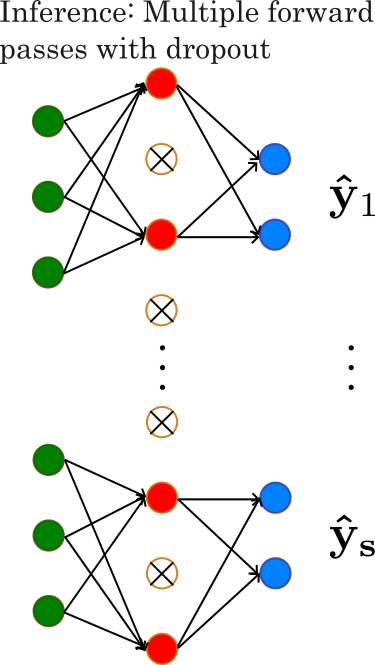
\includegraphics[width=0.33\textwidth]{figures/mcdropout.png}}%
      \begin{subfigure}{0.24\textwidth}
        \raisebox{\dimexpr.5\ht\largestimage-.5\height}{%
        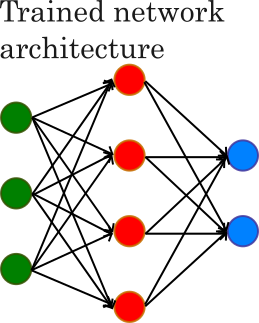
\includegraphics[width=\linewidth]{figures/mcdrop.png}}
        \caption{Original network}
        \label{fig:mcdrop1}
      \end{subfigure}
      \hfill
      \begin{subfigure}{0.33\textwidth}
        \usebox{\largestimage}
        \caption{MC Dropout}
        \label{fig:mcdrop2}
      \end{subfigure}
      \hfill
      \begin{subfigure}{0.33\textwidth}
        \raisebox{\dimexpr\ht\largestimage-\height}{%
        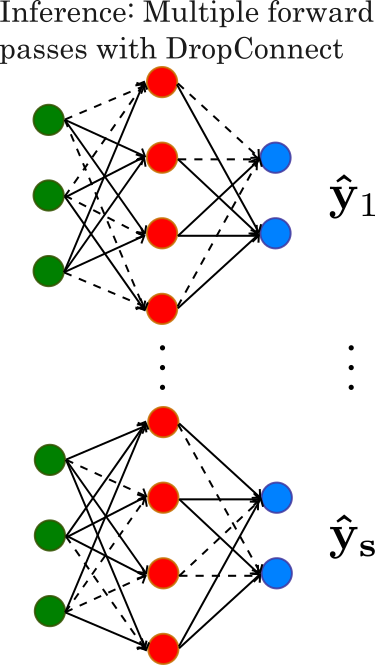
\includegraphics[width=\linewidth]{figures/mcdropconnect.png}}
        \caption{MC DropConnect}
        \label{fig:mcdrop3}
      \end{subfigure}
      \caption{Model uncertainty quantification using Monte Carlo dropout or DropConnect.}
      \label{fig:mcdrop}
    \end{figure}
    Dropout was introduced by~\cite{DropoutOG} as a stochastic regularization technique in NNs to prevent overfitting. By the properties of how dropout (randomly dropping out hidden units of inner layers in NN) is implemented, it also allows one to efficiently combine exponentially many different NNs without extra cost~\cite{DropoutOG}. Mathematically, for an input $x \in \mathbb{R}^d$ and a weight matrix $W\in \mathbb{R}^{d \times d'}$, a masking vector $m \in \mathbb{R}^{d'}$ is sampled whose each element is sampled independently from a Bernoulli distribution with some chosen probability $p$, then the hidden layer can be computed with activation function $a$ as $h = m \star a(Wx)$, where $\star$ refers to element-wise multiplication in this work.
    \newline

    DropConnect, the generalization of Dropout, was introduced by~\cite{DropConnectOG}. Similar to dropout, DropConnect also introduces randomness in the NN, but by randomly dropping a weight (a connection between two hidden units) instead of the hidden units. Mathematically, for an input $x \in \mathbb{R}^d$ and a weight matrix $W\in \mathbb{R}^{d \times d'}$, a masking matrix $M \in \mathbb{R}^{d \times d'}$ is sampled whose each element is sampled independently from a Bernoulli distribution with some chosen probability $p$, then the hidden layer can be computed with activation function $a$ as $h = a((M \star W) x)$.
    \newline

    ~\cite{DropoutUQ} showed that any NN of arbitrary depth with dropout or DropConnect incorporated into it approximates a familiar probabilistic model, namely deep Gaussian Process introduced in~\cite{DeepGP}.~\cite{DropConnectUQ} also showed a computationally tractable approximation of
    a Bayesian Neural Network (BNN) by using DropConnect. Such a probabilistic view allows one to estimate uncertainty using NNs with dropout or DropConnect~\cite{DropoutUQ, DropConnectUQ}. The mean and standard deviation associated with the prediction were empirically estimated for a test sample. The mathematical expression for this, when DropConnect is used, is provided, since it is the generalization of dropout. For a NN with the set of model weights $\theta = \{\theta_1, \ldots, \theta_M\}$, an $M$-dimensional vector of variables each following a Bernoulli distribution $S$ times $\{z^s_1, \ldots, z^s_M\}_{s=1}^S = \{z^s\}_{s=1}^S$ is sampled, corresponding to the model weights after dropping connections as $\{\theta^s_1, \ldots, \theta^s_M\}_{s=1}^S = \{\theta^s\}_{s=1}^S$. Then the mean can be estimated using the approximation given by Eq.~\ref{approxpreddist} as:
    \begin{equation}\label{MCDropMean}
        \mathbb{E}_{q(\mathbf{y^*|x^*})}(\mathbf{y^*}) \approx \frac{1}{S} \sum_{s=1}^S \mathbf{\hat{y}^*(x^*,\theta^s)}
    \end{equation}
    where $\mathbf{\hat{y}^*(x^*,\theta^s)}$ denotes the prediction of the NN with weights $\theta^s$ after DropConnect corresponding to the vector $z^s=\{z^s_1, \ldots, z^s_M\}$. This is equivalent to performing the NN forward pass $S$ times with different DropConnect sampling and averaging the predictions. This Monte Carlo estimate was termed MC DropConnect~\cite{DropConnectUQ} (MC Dropout~\cite{DropoutUQ} when dropout is used). Given that the data uncertainty $Cov_{p(\mathbf{y^*|x^*, \theta})}(y^*) = \sigma^2I$ is known, the predictive covariance can also be estimated as:
    \begin{equation}\label{MCDropVar}
        \mathbf{Var}_{q(\mathbf{y^*|x^*})}(\mathbf{y^*}) \approx \sigma^2I + \frac{1}{S} \sum_{s=1}^S \mathbf{\hat{y}^*(x^*,\theta^s)}^T \mathbf{\hat{y}^*(x^*,\theta^s)} - \mathbb{E}_{q(\mathbf{y^*|x^*})}(\mathbf{y^*})^T \mathbb{E}_{q(\mathbf{y^*|x^*})}(\mathbf{y^*})
    \end{equation}
    which comes from calculating the sample variance of the predictions from $S$ forward passes through the NN, with additional prediction uncertainty coming from the data (which can be ignored if assumed deterministic). Observe that for dropout, an $N$-dimensional vector of variables is sampled with each element sampled from a Bernoulli distribution where $N$ is the number of hidden nodes in the NN. The masked weights after dropout can be similarly computed based on the dropped hidden units instead of the dropped connections, and the same formulations given in Eq.~\ref{MCDropMean} and Eq.~\ref{MCDropVar} can be used to compute the empirical posterior mean and variance, respectively.
    \newline

    MC dropout or MC DropConnect has been a popular method in quantifying model uncertainty due to its simplicity and efficiency. There is no need to use a separate NN for approximation. With minimal modification to the existing network architecture, the uncertainty estimates can be computed by performing multiple forward passes during inference. As a result, there is no need to compromise accuracy by using approximate models. The authors of~\cite{BayesCNN} showed that simple dropout-based approximation fails for certain NN architectures such as Convolutional Neural Networks (CNNs), but the Bayesian interpretation of dropout (MC dropout approximation) helps alleviate this issue. But since all the NNs generated through dropout essentially come from the same parent NN, such methods are often limited in terms of capturing the diversity and approximating the original posterior, leading to underestimated variance and therefore poor uncertainty estimates as shown in~\cite{DropoutIssues1, DropoutIssues2}. For better estimates, many forward passes are required to be performed, which nullifies the cost-effectiveness of such methods~\cite{BayesCNN}. One also needs to be careful with the percentage of sparsity incorporated in the network via dropping out (e.g., high probability of dropping, or using dropout in every layer) as it might impose too strong regularization, resulting in slow learning and decreased accuracy~\cite{BayesSegNetUnc}. Still, due to the scalability in our use case, where we use deep learning models with many parameters, MC dropout or DropConnect are preferred instead of analytic approximation methods.
    


    \subsection{Deep Ensemble}\label{Deepsemble}
    An ensemble model combines the predictions of multiple individual models in some structured way to obtain the final prediction for an input. With the usage of accurate and diverse models, it can be assumed that the ensemble model achieves higher predictive accuracy than the individual models~\cite{EnsembleNN}. This holds for deep learning models too, as shown in~\cite{EnsembleNN, EnsembleNN2, EnsembleNN3}. Ensemble methods can not only improve predictive performance but also provide better-calibrated and more robust uncertainty estimates with capabilities to detect out-of-distribution (OOD) samples, as shown for Deep Ensembles introduced by~\cite{DeepEnsembleUQ}. Deep ensemble combines multiple deep NNs along with adversarial training~\cite{Adversarial} to smooth predictive distribution. Through the combination of multiple NNs, the deep ensemble also provides an empirical distribution over the predictions. So for an ensemble of $M$ NNs with weights or parameter sets $\theta_1, \ldots, \theta_M$ respectively, the predictive probability of output $\mathbf{y^*}$ given an input $\mathbf{x^*}$ can be computed as:
    \begin{equation}\label{EnsemblePred}
        p(\mathbf{y^*|x^*}) = \frac{1}{M} \sum_{m=1}^M p_{\theta_m}(\mathbf{y^*|x^*, \theta_m})
    \end{equation}
    for a uniformly weighted combination of the individual NN predictive probabilities parametrized by $\theta_m$ for $m \in \{1, \ldots, M\}$. In this frequentist approach, the prediction can be empirically estimated by averaging the predictions of the individual NNs, and the uncertainty can be computed by calculating the variance of these output predictions.
    \newline

    Several strategies for creating ensembles have been developed over the years. A review of general-purpose methods of constructing ensemble models can be found in~\cite{EnsembleReview}. For NNs, this can be differentiated based on the sources of uncertainty one wants to capture. An ensemble of different neural networks (NNs) can be constructed by using different parameter initializations, varying hyperparameters (e.g., learning rate, optimization strategy, regularization parameter)~\cite{HyperparEnsUnc}, or adjusting the number of layers, hidden nodes, or activation function. One can also keep the same NN architecture across different models, but randomize the data to learn different parameters by random shuffling of datasets or bootstrapping~\cite{DeepEnsembleUQ, NeuBoots}.
    \newline

    Like the dropout-based methods, deep ensemble methods are also easy to implement for estimating uncertainty. During training and inference, the process can be parallelized by training or inferring from each model separately at the same time. However, these methods still have a high computational and memory costs, which increase linearly with the number of models used in the ensemble in both training and inference, since one has to train or infer from and store multiple independent models in parallel. One also needs enough model diversity to ensure better uncertainty estimation from ensemble models. Several approaches have been developed~\cite{BatchEnsemble, Masksembles, PackedEnsemble} to address the bottleneck of memory and computational cost of standard ensemble methods. BatchEnsemble~\cite{BatchEnsemble} used efficient parametrization by using a shared weight matrix for all models and a rank-one matrix varying across different models for each connected layer, and therefore creates a member of the ensemble at each layer, which can be trained simultaneously. Masksembles~\cite{Masksembles} borrowed the idea of MC dropout, but instead of randomly dropping weights or nodes of the NN, Masksembles used a finite number of carefully chosen binary masks to be applied during training and inference. Packed-Ensembles~\cite{PackedEnsemble} used grouped convolutions proposed in AlexNet~\cite{AlexNet} to independently train subnetworks with fewer parameters within one base model.



\section{Implicit Generative Models}\label{ImplicitGen}
\begin{figure}[htb]
  \begin{center}
  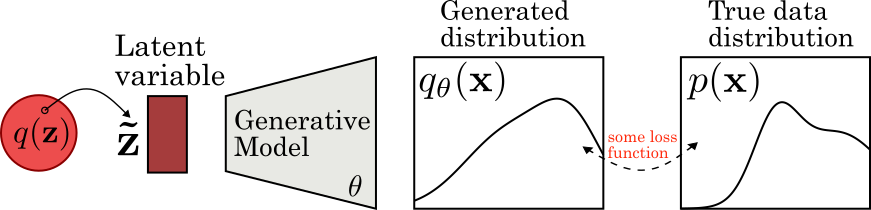
\includegraphics[width=\linewidth]{figures/implicitgen.png}
  \end{center}
  \caption{Learning implicit generative models.}\label{fig:implicit_gen}
\end{figure}
An implicit generative model is a stochastic process that can be used to directly simulate data from a probability distribution, and therefore it implicitly defines a probability distribution. As implicit generative models do not provide an explicit parametric specification of the
distribution of an observed random variable $\mathbf{x}\in \mathbb{R}^d$, the likelihood is often intractable. These models can also be thought of as latent variable models since they use a latent variable $\mathbf{\tilde{z}} \in \mathbb{R}^m$ and apply a deterministic function $\mathcal{G}_\theta: \mathbb{R}^m\rightarrow \mathbb{R}^d$ parametrized by $\theta$ on the latent variable $\mathbf{\tilde{z}}$ mapping it to a sample in the distribution. This can be formulated as:
\begin{equation}\label{IGM}
    \mathbf{\tilde{z}} \sim q(\mathbf{z}), \quad \mathbf{x} =  \mathcal{G}_\theta(\mathbf{\tilde{z}})
\end{equation}
where the latent variable is generated from a fixed, simple distribution such as a standard Gaussian ($\mathbf{\tilde{z}} \sim \mathcal{N}\left(0, I_m\right)$). We can effectively approximate the original data distribution $p(\mathbf{x})$ by computing the likelihood specified by Eq.~\ref{IGM}:
\begin{equation}\label{IGMLikelihood}
    p(\mathbf{x}) \approx q_\theta(\mathbf{x}) = \frac{\partial}{\partial x_1} \cdots \frac{\partial}{\partial x_d} \int_{\mathcal{G}_\theta(\mathbf{z}) \leq \mathbf{x}} q(\mathbf{z}) d\mathbf{z}
\end{equation}
for $\mathbf{x}=\{x_1, \ldots, x_d\}$. 
\\
If $\mathcal{G}$ is invertible, or has easily characterised roots with the data space having the same dimension as the latent space, the rules of transformation of probability density can be applied to compute the generated distribution~\cite{LearnIGM}. But such functions limit the capabilities of modelling more complex distributions. Therefore, more general functions are preferred, such as a differentiable function specified by a deep NN. In such cases, Eq.~\ref{IGMLikelihood} is often intractable. Therefore, methods that approximate the likelihood in Eq~\ref{IGMLikelihood} or completely avoid using the likelihood must be implemented. An extensive discussion about such methods is done in~\cite{LearnIGM}.


    

\section{Gaussian Process}\label{GP}
A Gaussian process (GP) is a generalization of the Gaussian distribution extended to an infinite number of dimensions. A probability distribution describes the probability of different values (scalar or vector) a random variable (univariate or multivariate) can take. On the other hand, a stochastic process determines the properties a random function follows. According to the above definitions, a Gaussian process can be considered as a stochastic process over infinite-dimensional functions or an infinite collection of random variables, any finite number of which follow a joint Gaussian distribution~\cite{GPML}. So, given a finite set of points, a Gaussian process can provide us probability distribution over possible functions that fit those points. Evidently, GP is a non-parametric model. 
\newline

Now, let $\mathcal{F}=\{f(\mathbf{x})\}_{\mathbf{x} \in D}$ be a collection of random variables for some continuous value $\mathbf{x} \in D \subset \mathbb{R}^d$. Therefore by definition, $\mathcal{F}$ is a Gaussian process if for any two values $\mathbf{x}, \mathbf{x}^{\prime} \in D \subset \mathbb{R}^d$,

\begin{equation}\label{GPDef}
    f(\mathbf{x}), f\left(\mathbf{x}^{\prime}\right) \sim \mathcal{N}\left(\left[\begin{array}{c}
    m(\mathbf{x})  \tag{1}\\
    m\left(\mathbf{x}^{\prime}\right)
    \end{array}\right],\left[\begin{array}{cc}
    k(\mathbf{x}, \mathbf{x}) & k\left(\mathbf{x}, \mathbf{x}^{\prime}\right) \\
    k\left(\mathbf{x}^{\prime}, \mathbf{x}\right) & k\left(\mathbf{x}^{\prime}, \mathbf{x}^{\prime}\right)
    \end{array}\right]\right)
\end{equation}
for some mean function $m(\mathbf{x})$ and covariance function $k\left(\mathbf{x}, \mathbf{x}^{\prime}\right)$ where $m: D \rightarrow \mathbb{R}, k: D \times D \rightarrow \mathbb{R}$ uniquely specify the Gaussian process $\mathcal{F}$. The mean and the covariance functions of the actual Gaussian process $f(\mathbf{x})$ can be defined as:
\begin{align}\label{GPFunc}
    m(\mathbf{x}) & =\mathbb{E}[f(\mathbf{x})]  \\
    k\left(\mathbf{x}, \mathbf{x}^{\prime}\right) & =\mathbb{E}\left[(f(\mathbf{x})-m(\mathbf{x}))\left(f\left(\mathbf{x}^{\prime}\right)-m\left(\mathbf{x}^{\prime}\right)\right)\right]
\end{align}
The Gaussian process is denoted as:
\begin{equation}\label{GPForm}
f(\mathbf{x}) \sim \mathcal{G} \mathcal{P}\left(m(\mathbf{x}), k\left(\mathbf{x}, \mathbf{x}^{\prime}\right)\right)
\end{equation}
Given a dataset $\mathbf{X=\{x_n\}_{n=1}^N, Y=\{y_n\}_{n=1}^N}$, where $\forall n \in \{1, \ldots, N\}$, $\mathbf{y_n}$ is an observed instance of the GP defined by the function $f$, and a set of new points $\mathbf{X^*=\{x^*_n\}_{n=1}^{N^*}}$ the joint distribution of the test points and observed points $\left[f(\mathbf{X^*, X})\right]^T$=$\left[f\left(\mathbf{x^*}_{1}\right), \ldots, f\left(\mathbf{x^*_{N^*}}\right), f\left(\mathbf{x}_{1}\right), \ldots, f\left(\mathbf{x_{N}}\right)\right]^T$ according to the GP prior can be written as:
{\small\begingroup
\renewcommand{\arraystretch}{1.25}
\setlength\arraycolsep{0.5pt}
\begin{equation}\label{GPJointBig}
    \mathcal{N}\left(\left[\begin{array}{c}
        m\left(\mathbf{x^*}_{1}\right)\\
        \vdots \\
        m\left(\mathbf{x^*_{N^*}}\right)\\
        m\left(\mathbf{x}_{1}\right)\\
        \vdots \\
        m\left(\mathbf{x_{N}}\right)
        \end{array}\right],
        \left[
        \begin{array}{cccccc}
        k\left(\mathbf{x^*}_{1}, \mathbf{x^*}_{1}\right) & \ldots & k\left(\mathbf{x^*}_{1}, \mathbf{x^*}_{N^*}\right) & k\left(\mathbf{x^*}_{1}, \mathbf{x}_{1}\right) & \ldots & k\left(\mathbf{x^*}_{1}, \mathbf{x}_{N}\right) \\
         \vdots & \ddots & \vdots & \vdots & \ddots & \vdots \\
        k\left(\mathbf{x^*}_{N^*}, \mathbf{x^*}_{1}\right) & \ldots & k\left(\mathbf{x^*}_{N^*}, \mathbf{x^*}_{N^*}\right) & k\left(\mathbf{x^*}_{N^*}, \mathbf{x}_{1}\right) & \ldots & k\left(\mathbf{x^*}_{N^*}, \mathbf{x}_{N}\right) \\
        k\left(\mathbf{x}_{1}, \mathbf{x^*}_{1}\right) & \ldots & k\left(\mathbf{x}_{1}, \mathbf{x^*}_{N^*}\right) & k\left(\mathbf{x}_{1}, \mathbf{x}_{1}\right) & \ldots & k\left(\mathbf{x}_{1}, \mathbf{x}_{N}\right) \\
        \vdots & \ddots & \vdots & \vdots & \ddots & \vdots \\
        k\left(\mathbf{x}_{N}, \mathbf{x^*}_{1}\right) & \ldots & k\left(\mathbf{x}_{N}, \mathbf{x^*}_{N^*}\right) & k\left(\mathbf{x}_{N}, \mathbf{x}_{1}\right) & \ldots & k\left(\mathbf{x}_{N}, \mathbf{x}_{N}\right)
        \end{array}
        \right]\right)
\end{equation}
\endgroup
}
which can be rewritten as
\begin{equation}\label{GPJointConcise}
        \left[\begin{array}{l}
        f\left(\mathbf{X^*}\right)\\
        f\left(\mathbf{X}\right)
    \end{array}\right] \sim \mathcal{N}\left(\left[\begin{array}{c}
        m\left(\mathbf{X^*}\right)\\
        m\left(\mathbf{X}\right)
        \end{array}\right],
        \left[\begin{array}{cc}
        k\left(\mathbf{X^*}, \mathbf{X^*}\right) & k\left(\mathbf{X^*}, \mathbf{X}\right) \\
        k\left(\mathbf{X}, \mathbf{X^*}\right) & k\left(\mathbf{X}, \mathbf{X}\right) \\
        \end{array}\right]\right)
\end{equation}
From this probabilistic formulation, the posterior distribution over functions for new pointd can be easily computed by conditioning the joint prior distribution on the observations:
\begin{equation}\label{GPPosterior}
    \begin{aligned}
        f\left(\mathbf{X^*} \mid \mathbf{X, Y}\right) \sim \mathcal{N}(m\left(\mathbf{X^*}\right)+k\left(\mathbf{X^*}, \mathbf{X}\right) k\left(\mathbf{X}, \mathbf{X}\right)^{-1}\left(\mathbf{Y}-m\left(\mathbf{X}\right)\right),\\
        k\left(\mathbf{X^*}, \mathbf{X^*}\right)-k\left(\mathbf{X^*}, \mathbf{X}\right) k\left(\mathbf{X}, \mathbf{X}\right)^{-1} k\left(\mathbf{X}, \mathbf{X^*}\right))
    \end{aligned}
\end{equation}
Usually, a zero mean ($m(\mathbf{x})=0$) is assumed for the GP prior. If the mean is not zero, the data can always be centred, or the Gaussian process $f-m$ can be considered. In case of a zero mean prior, the posterior in Eq.~\ref{GPPosterior} becomes:
\begin{equation}\label{GPPosterior0}
    \begin{aligned}
        f\left(\mathbf{X^*}\right) \mid \mathbf{X, Y} \sim \mathcal{N}(k\left(\mathbf{X^*}, \mathbf{X}\right) k\left(\mathbf{X}, \mathbf{X}\right)^{-1}\mathbf{Y}, \\
        k\left(\mathbf{X^*}, \mathbf{X^*}\right)-k\left(\mathbf{X^*}, \mathbf{X}\right) k\left(\mathbf{X}, \mathbf{X}\right)^{-1} k\left(\mathbf{X}, \mathbf{X^*}\right))
    \end{aligned}
\end{equation}
\newline

However, in real-life settings, one does not have access to the ground-truth function values. Only some noisy values are observed which can be modelled as $\mathbf{y} = f(\mathbf{x}) + \varepsilon$ for some observed input $\mathbf{x}$ where the noise $\varepsilon$ is assumed to follow a Gaussian distribution, $\varepsilon \sim \mathcal{N}(0, \sigma^2_N I)$ for the $N$ observed data points. It is known that the sum of two Gaussian distributions is also Gaussian for two independent Gaussian random variables with the mean and the covariance equal to the sum of the means and covariances of the two Gaussians. Therefore, for the independent identically distributed Gaussian noise, the prior covariance becomes $k\left(\mathbf{X^*}, \mathbf{X^*}\right) + \sigma^2_N I$, and then the joint distribution and the posterior can be rewritten by replacing $k\left(\mathbf{X^*}, \mathbf{X^*}\right)$  with $k\left(\mathbf{X^*}, \mathbf{X^*}\right) + \sigma^2_N I$.
\newline

The covariance function is a critical component of a Gaussian process since it encodes the prior assumptions about the function to be learnt regarding similarity between the data points~\cite{GPML}. Intuitively, similar inputs are expected to have similar outputs. The covariance function indicates how closely a certain input is related to other observed points, and only the close points will have significant contributions to the output prediction. There are many possible choices for the covariance function depending on the application and our prior knowledge about the function. A comprehensive list of potential covariance functions can be found in~\cite{GPML}.


\section{Contrastive Learning}\label{Contrast}
Contrastive learning is a method of learning an embedding space from data that maintains the pairwise similarity between data points. The idea is to find a function that maps inputs into outputs in a target space, such that similar pairs remain similar according to some similarity metric and dissimilar pairs are separated. The target embedding space approximates the semantic distance inherent in the input space. One can observe that contrastive learning only requires semantic relationships of similarity and does not need any distance measure in the input space~\cite{PairMarginCL}. Such a mapping can be learnt by minimizing an appropriate discriminative loss function, called the contrastive loss function. One of the earliest works to introduce such an objective~\cite{ContLoss} applied contrastive learning to a face verification task.~\cite{PairMarginCL} used the same idea for dimensionality reduction, which is useful for dealing with high-dimensional data similar to this work. Due to numerical precision issues encountered in computing the Gaussian process posterior or even marginal likelihood, contrastive learning can provide an alternative approach to learn a feature mapping for points without requiring likelihood computation, as a means of prior separation of dissimilar points before modeling a GP. Moreover, although contrastive learning has been more impactful in self-supervised learning, recent works have also seen a rise in applications in supervised learning~\cite{SelfSupervisedCont, SupervisedCont}. 
\newline

Earlier works mostly focused on loss involving pairs (positive and negative) of samples, but later works have introduced various new contrastive loss functions useful for different applications. In this work, the contrastive losses used will be the triplet loss introduced in~\cite{TripletLoss}, sigmoid loss used in language-image pair pre-training~\cite{SigLIP}, and a discriminative loss based on spacetime distance used in~\cite{SpaceMesh}.
\newline

Triplet loss considers triplets of data points where an anchor is selected along with a positive and a negative sample for which the function $\mathbf{f}$ maps the positive instance close to the anchor and the negative one farther away according to some distance metric. Euclidean distance is usually selected as the metric in the target space. So for any anchor $\mathbf{x^a_i}$, positive sample $\mathbf{x^p_i}$ and negative sample $\mathbf{x^n_i}$ in a set of triplets $\mathcal{T} = \mathbf{\left(x_{i}^{a}, x_{i}^{p}, x_{i}^{n}\right)_{i=1}^N}$, it is desired that:
\begin{equation}\label{tripletcondition}
    \left\|\mathbf{f(x_{i}^{a})-f(x_{i}^{p})}\right\|_{2}^{2}+\epsilon<\left\|\mathbf{f(x_{i}^{a})-f(x_{i}^{p})}\right\|_{2}^{2}, \forall\left(\mathbf{x_{i}^{a}, x_{i}^{p}, x_{i}^{n}}\right) \in \mathcal{T} 
\end{equation}
where $\epsilon$ is the margin enforced between positive and negative pairs. Then the triplet loss can be defined as:
\begin{equation}\label{tripletloss}
    \mathcal{L}(\mathbf{f}, \mathcal{T}) = \sum_{\mathbf{i=1}}^\mathbf{N} \max \left(\left\|\mathbf{f(x_{i}^{a})-f(x_{i}^{p})}\right\|_{2}^{2} - \left\|\mathbf{f(x_{i}^{a})-f(x_{i}^{n})}\right\|_{2}^{2} +\epsilon, 0\right) .
\end{equation}
\newline

On the other hand, sigmoid loss in language-image pair pre-training and spacetime distance-based contrastive loss cannot be directly used in this work. Details of the modified formulations to these losses are provided in Chapter~\ref{ch:methods}.

\chapter{Related Works}\label{ch:related-work}
Previous research that is relevant to our work can be roughly categorized into the following fields:



\section{Point Cloud-based Methods}\label{PCC-old}
Due to the ease of procuring, point clouds have been the most popular representation used for tasks related to 3D shapes. A similar trend was also observed for 3D shape completion tasks. On the other hand, with the increasing success of deep learning models in various domains, numerous works have also focused on utilizing deep neural networks for 3D shape learning tasks. Point cloud completion is also one of many such applications. Several previous works~\cite{PCN, PoinTr, PointAttN, VarPCN, PCNSkip, Snowflake} performed point cloud completion for a given partial point cloud by predicting the complete point cloud or the missing points in the cloud. 
\\
Point Completion Network (PCN)~\cite{PCN} was the first such approach that generated a complete cloud directly from the incomplete point cloud without using any voxelization techniques. PCN used an autoencoder (encoder-decoder) network to produce a denser point cloud as output in multiple stages. Other methods use variational autoencoder~\cite{VarPCN}, transformer-based encoder-decoder~\cite{PoinTr, Snowflake}, attention-based autoencoder~\cite{PointAttN, VarPCN, PCNSkip} for completion tasks. A complete review of all point cloud completion methods is not possible here. A comprehensive survey of such techniques can be found in~\cite{PCNSurvey}. 
\newline

However, the methods mentioned above are inherently deterministic with an injective mapping between partial and complete clouds, which is impractical for our purpose. Due to the inherent uncertainty of the completion process, one partial cloud can map to different complete shapes. Various works have approached this as a generative modeling task to incorporate the implicit ambiguity of the missing points. Generative Adversarial Networks (GANs)~\cite{GAN} have been the most popular generative modeling technique ever since it was introduced, and the same idea was also explored for point cloud completion in~\cite{GANPCC1, GANUPCC}. While the usage of GAN employed standard learning for partial and complete pairs in~\cite{GANPCC1}, the application was extended to unpaired point cloud completion in~\cite{GANUPCC}. However, those early works did not explore the idea of generating point clouds with uncertainty. 
\newline

For supervised point completion, generating multiple shapes from a single partial shape is difficult, since we only have one complete ground truth shape available for each partial input during training. Authors of~\cite{CGAN} addressed this issue by using a conditional generative adversarial network (c-GAN) along with a variational autoencoder (VAE) to learn to generate multiple complete clouds during inference. But because of mode collapse in GANs~\cite{ModeCollapseGAN}, generated shapes are often not geometrically diverse and differ only in simpler aspects such as length or width. Another approach~\cite{PCCIMLE} used implicit maximum likelihood estimation (IMLE) introduced in~\cite{IMLE} instead of GANs to incorporate multiple completions for an input partial shape without the downside of mode collapse. 
\\
Authors of~\cite{HyperPocket} predicted the missing parts of the shapes rather than generating complete shapes by enforcing the representation of the missing point cloud space to follow a predetermined probability distribution and using a hypernetwork~\cite{Hypernet} to train a decoder that takes the concatenated representations of the partial and missing points and outputs weights of the target network. The target network is trained to produce a complete point cloud from a simple probability distribution as implemented in~\cite{PCHypernet}. Another method~\cite{EBResLT} proposed incorporating an energy-based model (EBM)~\cite{EBM} to transport the partial cloud representation to the complete cloud representation using residual (the difference between partial and complete representations) in an unsupervised setting. Although these methods addressed the issue of the inherent non-determinism of point cloud completion, none except one~\cite{EBResLT} produced any output that can help quantify the uncertainty of such completions.


\section{Implicit Neural Representation-based Methods}\label{INR-old}
Another popular representation for 3D shapes used in recent works is an implicit function whose zero level set describes the underlying surface. Implicit function is memory-efficient and easy to evaluate once known, making it preferable over other representations such as voxels or point clouds. Consequently, numerous works have performed surface reconstruction from point clouds by recovering the implicit representation of the surface. Similar to point cloud completion, deep learning methods have also found considerable success in learning implicit representations of surfaces. We refer to these as implicit neural representations (INRs). Most of the existing works assume that normal information is available and use that to enforce some kind of geometric prior. These methods rely quite significantly on the normal information-based constraints to produce better results. But in our work, we are only interested in the works that predict an implicit representation from unoriented point clouds. These methods utilize different regularization techniques based on the available data. 
\newline

Sign agnostic learning introduced in~\cite{SAL} used the readily available unsigned distance values for points normally distributed around observed points by computing the distance to the nearest point in the point cloud, and used a differentiable sign-agnostic monotonic function as the loss function to recover the unsigned distance function. Sign agnostic learning with derivatives~\cite{SALD} extended this method to further include a term based on the gradients of the distance functions in the loss function and showed that the regularization based on gradients resulted in better learning. Implicit geometric regularization~\cite{IGR} enforced the gradients of the implicit function to have unit norm. Neural-Pull method~\cite{NeuralPull} sampled query points normally distributed around the ground truth point cloud and computed the pulled location of the query points based on the predicted distance function and its gradient to minimize the distance between the pulled locations and the closest point on the surface. Divergence-guided shape implicit neural representation~\cite{DiGS} minimized the magnitude of the divergence or Laplacian of the distance field as an added regularization. Neural Singular Hessian method~\cite{NeuralHessian}, on the other hand, constrained the Hessian matrix of the implicit function to have zero determinant for points on and close to the surface as a geometric prior, leading to state-of-the-art results for recovering INR from unoriented point clouds.


\section{Gaussian Process-based Methods}\label{Stoch-old}
Gaussian process is the most commonly used method for uncertainty quantification for regression tasks. Since learning the distance function of a 3D shape can be considered as a regression problem, many methods have tried to model the implicit function as a Gaussian process. The known distance function values act as observations of the GP and thus can be used to predict the distance values at other query points by computing the posterior distribution. The variance of the posterior distribution also quantifies the corresponding uncertainty of the predicted distance values. Such a representation of surfaces is referred to as Gaussian Process Implicit Surface (GPIS). GPIS was first introduced in~\cite{GPIS} where the supervision is done by fixing the distance values of points on the surface to zero and sampling virtual points inside and outside the surface with -1 and +1 distance values. Even with the discrete measurements, the surface can be recovered due to the interpolation abilities of GP regression. Kernels or covariance functions are an important part of GP regression that indicate the similarity between two points in shape and directly affect the posterior distribution. The authors of~\cite{GPIS} used a covariance function equivalent to the thin plate spline energy regularizer, which minimizes the overall curvature of the learned implicit function. 
\newline

Although distance field estimation using standard GPIS methods is accurate close to the surface, it does not hold as we move away from the surface due to the lack of training points, with the field converging to zero even far from the surface~\cite{logGPIS}. Inspired by the heat method proposed in ~\cite{GeodesicHeat}, authors of~\cite{logGPIS} suggested using the logarithm of standard GP regression to model the implicit surface termed as log-GPIS. But apart from log-GPIS not producing a true Euclidean distance field, it sacrifices interpolation abilities on the surface for accurate distance field estimation away from the surface~\cite{onlinePriorGPIS}. Moreover, the logarithmic transformation affects the precision of uncertainty quantification. Another work proposed an alternative formulation of the distance field as a reverse of a latent scalar field modelled by GP, where the reverting function corresponds to the inverse of the GP kernel~\cite{GPDF}.
\newline

In terms of performance, most of these methods suffer due to the cubic complexity of GP, and limiting the number of points to decrease computational cost might affect robustness. Several works~\cite{mixGPOccMap, locGPOccMap, onlineGPIS} have tried to solve the computational complexity issue by using multiple GPs, each modelled locally on partitioned clusters. Authors of~\cite{onlinePriorGPIS} used a distance field prior extracted from simpler geometric features on the GP mean function to reduce the model complexity. Another method~\cite{GMMGP} used a Gaussian Mixture Model (GMM) based prior instead of a geometrically extracted prior for the same purpose.
\newline

Stochastic Poisson Surface Reconstruction~\cite{SPSR} combined PSR with GP to formulate a stochastic version of PSR where the observed points along with the normal information in a point cloud are considered as observations of a GP. Therefore, a local GP is used to approximate the distribution of the gradient vector field. The GP posterior, in turn, gives us the mean and covariance functions of the vector field. Then we can recover the mean and covariance functions of the scalar field from those of the vector field using a global PDE solver~\cite{SPSR}. While in~\cite{SPSR} the authors used a standard PDE solver, in~\cite{NeuralSPSR} the authors replaced it with a neural PDE solver by parametrizing the mean and covariance of the implicit scalar field using an NN and optimizing it using gradient descent on losses defined from the variational version of the Poisson equation. This formulation allowed us even to extend to the screened version defined in~\cite{ScreenedPSR} by incorporating the screening terms in the loss function, as well as removing the complex discretization process needed for the standard PDE solvers~\cite{NeuralSPSR}. 

%%%%%%%%%%%%%%%%%%%%%%%%%%%%%%%%%%%%%%%%%%%%%%%%%%%%%%%%%%%%%%%%%%%%%%%%%%%%%%%%%%%%%%%%%%%%%%%%%%%%%

\chapter{Methods}\label{ch:methods}
This chapter introduces the different methods used to quantify uncertainty for curved surfaces from partial point clouds without any extra information available. The task can be formulated for two different scenarios regarding the availability of additional data or prior information related to the 3D shape. In case of prior knowledge or additional data being unavailable, only the point cloud collected from multiple scans of the object can be used. Then our task can be defined as:
\begin{problemnotitle}{SingleCloud}{}
    \probleminput{A point cloud with $N_C$ points represented by $\mathbf{X}=\left\{\mathbf{x}_{i} \in \mathbb{R}^{3}\right\}_{i=1}^{N_C}$.}
    \problemoutput{A probabilistic estimate of the distance from the surface or probability of lying on the surface for any point $\mathbf{x} \in \mathbb{R}^{3}$.}
\end{problemnotitle}
\newline

On the other hand, if it is assumed that the kind of object the 3D shape belongs to is known, an additional dataset of related 3D shapes with partial and complete point clouds can be used. Then for a dataset of partial point clouds $\mathbf{X_P} \in \mathbb{R}^{N \times N_P \times 3}$ with $N$ instances of $N_P$ points in each incomplete point cloud instance, a corresponding dataset of complete point clouds $\mathbf{X_C} \in \mathbb{R}^{N \times N_C \times 3}$ with $N$ instances of $N_C$ points in each ground truth complete point cloud instance is available. Then the problem statement becomes:
\begin{problemnotitle}{DataCloud}{}
    \probleminput{A partial point cloud with $N_P$ points represented by $\mathbf{X}=\left\{\mathbf{x}_{i} \in \mathbb{R}^{3}\right\}_{i=1}^{N_P}$.}
    \problemoutput{A probabilistic estimate of the distance from the surface or probability of lying on the surface for any point $\mathbf{x} \in \mathbb{R}^{3}$.}
\end{problemnotitle}
\newline

Then the learned distribution over the distance field or the probabilistic surface reconstruction can be used for further downstream tasks.


\section{Empirical Uncertainty Quantification for Point Cloud Completion}\label{euqpcc}
In this section, a solution to the Problem~\ref{DataCloud} is proposed utilizing a point cloud completion method for the given input partial cloud. Instead of directly computing the probabilistic estimate of the underlying surface, multiple possible completions are generated from the input and then the surface along with the associated uncertainty is empirically estimated by matching points between generated complete clouds. The partial cloud is denoted by $\tilde{X}=\left\{\mathbf{\tilde{x}}_{i} \in \mathbb{R}^{3}\right\}_{i=1}^{N_P}$ and the generated complete cloud by $\hat{X}=\left\{\mathbf{\hat{x}}_{i} \in \mathbb{R}^{3}\right\}_{i=1}^{N_C}$. So the aim is to learn $p(\hat{X}|\tilde{X})$. During training, there is access to the ground truth complete cloud, which is denoted by $X=\left\{\mathbf{x}_{i} \in \mathbb{R}^{3}\right\}_{i=1}^{N_C}$. Since for any partial cloud, there are many possible complete clouds consistent with the partial cloud, one needs to learn to generate non-deterministic predictions depending upon some source of randomness. In Chapter~\ref{ch:background}, different ways to quantify uncertainty in deep learning models were reviewed, which provided an idea about how similar methods can also be implemented to generate different predictions with randomness. But first, the standard architecture used for point completion should be described.


    \subsection{General Structure of Point Completion Network}
    \begin{figure}[htb]
      \begin{center}
      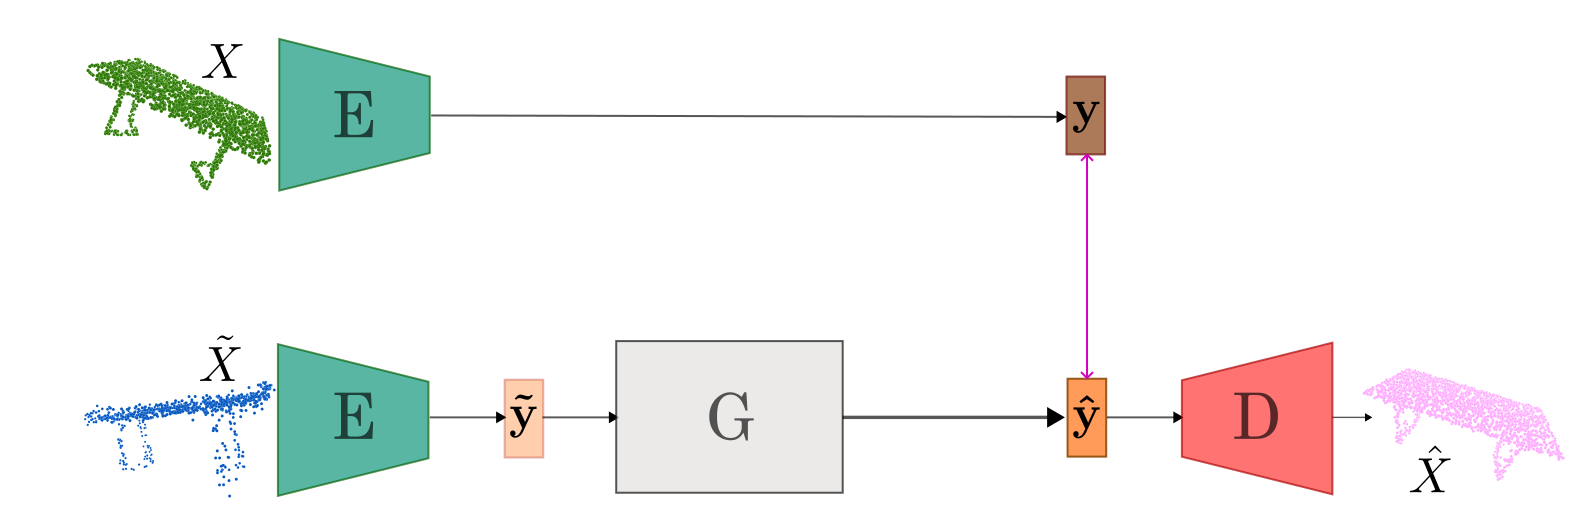
\includegraphics[width=\linewidth]{figures/general_network.png}
      \end{center}
      \caption{General structure of network used for training point cloud completion. During training, ground truth complete cloud $X$ is input to the encoder E to output the encoding $\mathbf{y}$. Parallelly partial cloud $\tilde{X}$ is input to the encoder E to generate the encoding $\mathbf{\tilde{y}}$, which is then given to generator G outputting new encoding $\mathbf{\hat{y}}$ which is compared to $\mathbf{y}$. The decoder D, on the other hand, produces a complete cloud $\hat{X}$ from  $\mathbf{\hat{y}}$.}\label{fig:gen_net}
    \end{figure}
    The general structure of the network used for point cloud completion consists of an auto-encoder (encoder-decoder network) and a generator network. The encoder is denoted by E, the decoder by D, and the generator by G (see Figure~\ref{fig:gen_net}). Through the auto-encoder network's encoder, one can encode the partial shape represented by $\tilde{X}$ and the complete shape represented by $X$ to obtain the encodings $\mathbf{\tilde{y}}$ and $\mathbf{y}$, respectively. 
    \\
    Meanwhile, generator G generates a new encoding $\mathbf{\hat{y}}$ from the partial shape encoding $\mathbf{\tilde{y}}$ from which the decoder can produce a new complete shape $\hat{X}$. Generator G plays the role of the network that incorporates the randomness of the completion method, as it enables the generation of different encodings from the partial cloud encoding through G. Then, different complete clouds can be produced via the decoder, and the uncertainty of our completion method can be empirically estimated from the generated clouds. In the following section, the implementation details of the above idea is described.

    
    \subsection{Uncertainty in Encoding Generation}
        \subsubsection{MC Dropout or DropConnect in Generator}
        \begin{figure}[htb]
          \begin{center}
          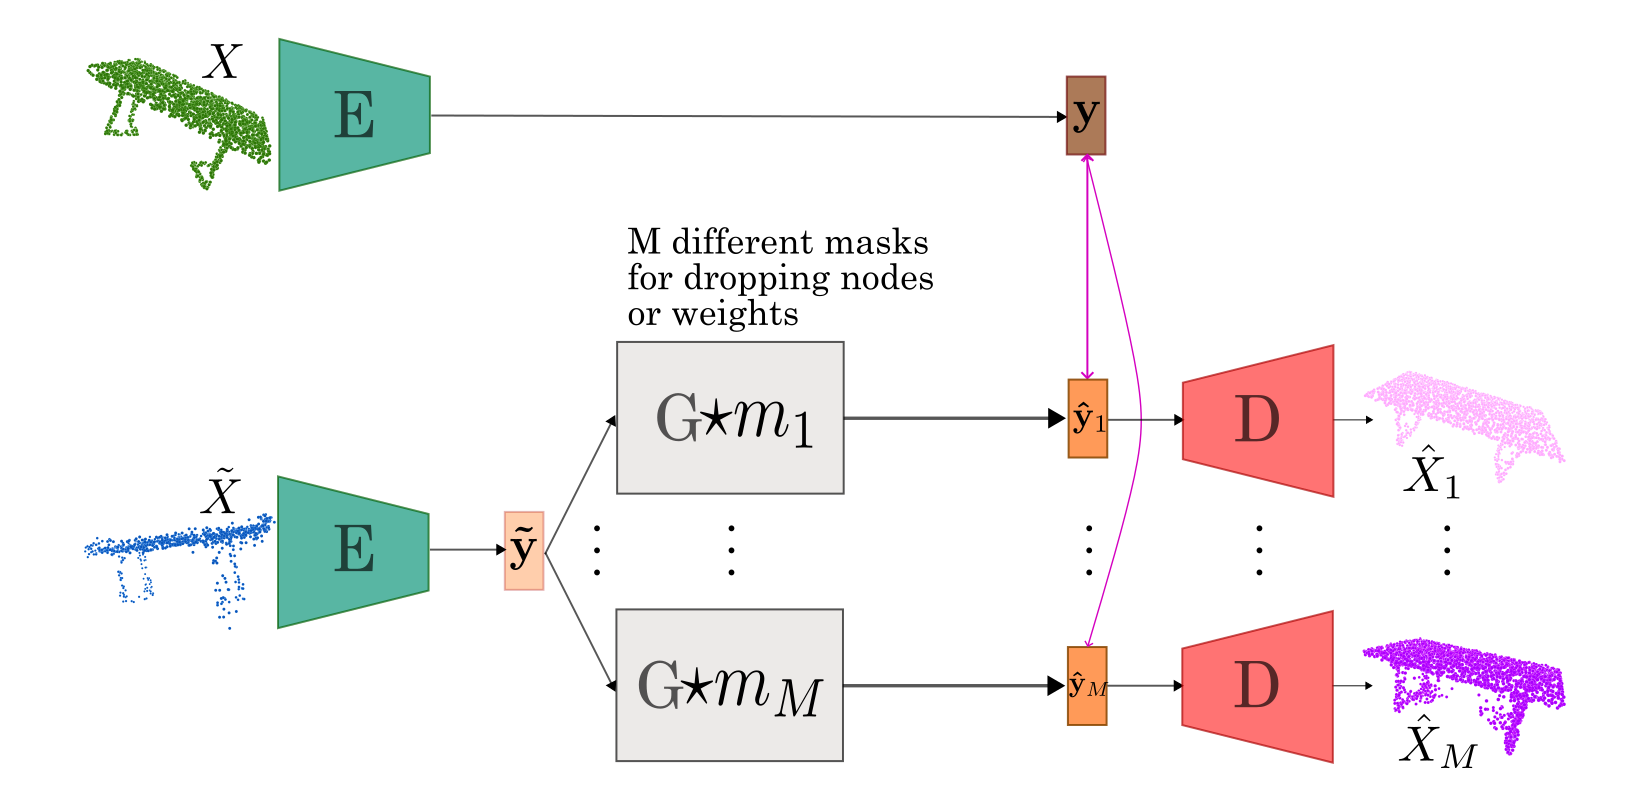
\includegraphics[width=\linewidth]{figures/drop_network.png}
          \end{center}
      \caption{Network for point cloud completion uncertainty quantification using dropout or DropConnect. During inference, the original generator network is modified based on some masking ($\{m_i\}_{i=1}^M$) multiple times to produce different generators.}\label{fig:drop_net}
        \end{figure}
        One simple idea to generate different encodings via the generator is to use dropout or DropConnect in the generator network while training. As explained in section~\ref{MCDrop}, dropout or DropConnect can also be used during inference to generate different encodings and complete shapes corresponding to those encodings for a particular input partial cloud (see Figure~\ref{fig:drop_net}). 
        
        \subsubsection{Deep Ensemble of Generators}
        \begin{figure}[htb]
          \begin{center}
          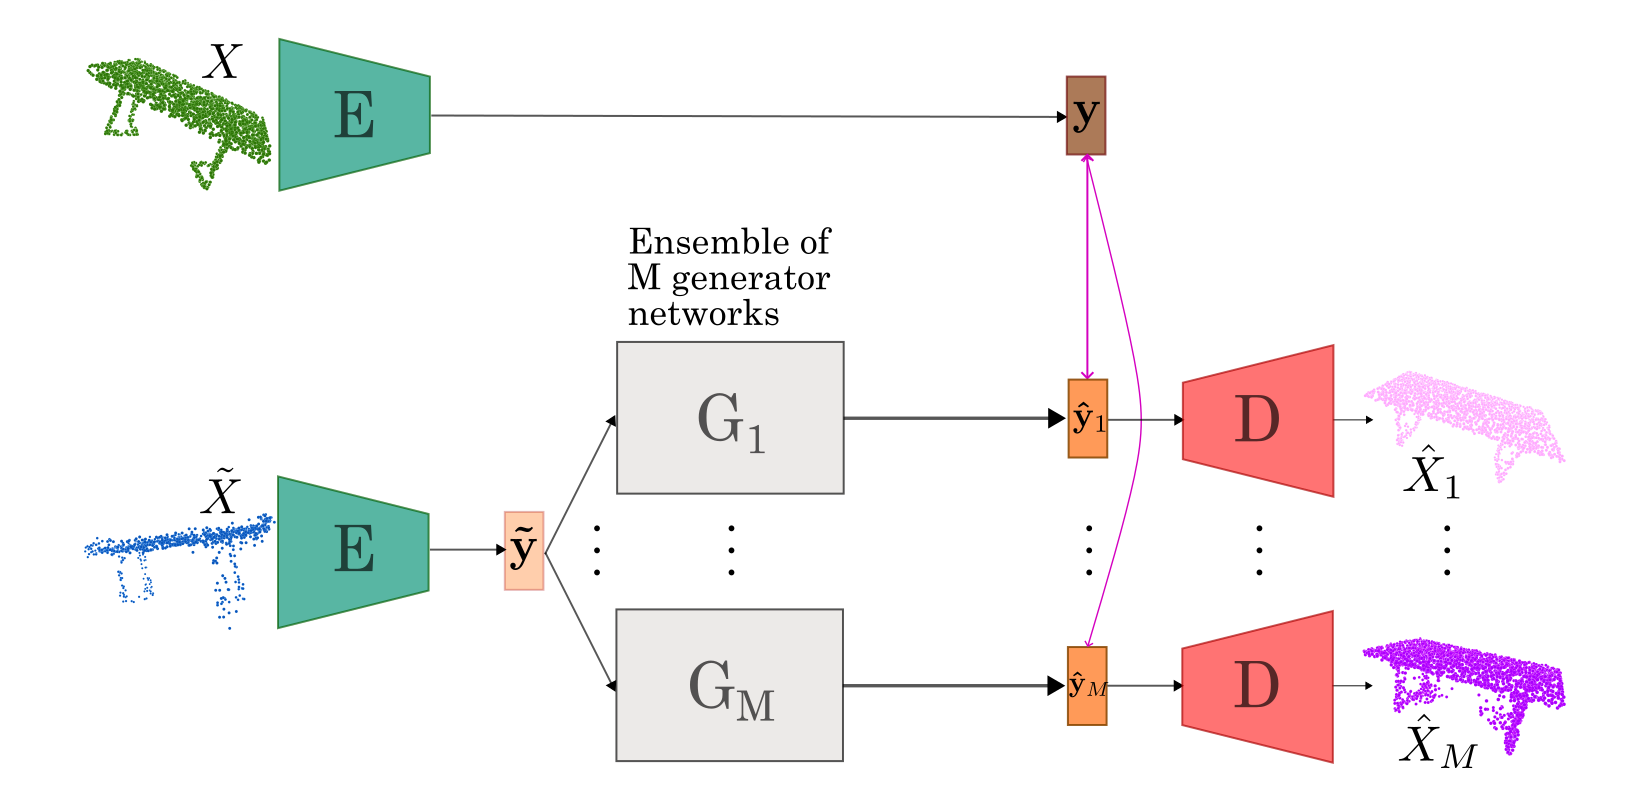
\includegraphics[width=\linewidth]{figures/ensemble_network.png}
          \end{center}
          \caption{Network for point cloud completion uncertainty quantification using deep ensemble. Different generators (based on the ensemble construction strategy) are trained. During inference, different generators produce different encodings.}\label{fig:ens_net}
        \end{figure}
        An ensemble of generators can be used to train the point completion network. As described in section~\ref{Deepsemble}, there are many ways to construct the ensemble of generators. Different initializations of parameters were used in this work to create the ensemble. During inference, each generator in the ensemble outputs a different encoding, giving us different complete shapes(see Figure~\ref{fig:ens_net}).

        \subsubsection{Conditional Implicit Generative Model}
        \begin{figure}[htb]
          \begin{center}
          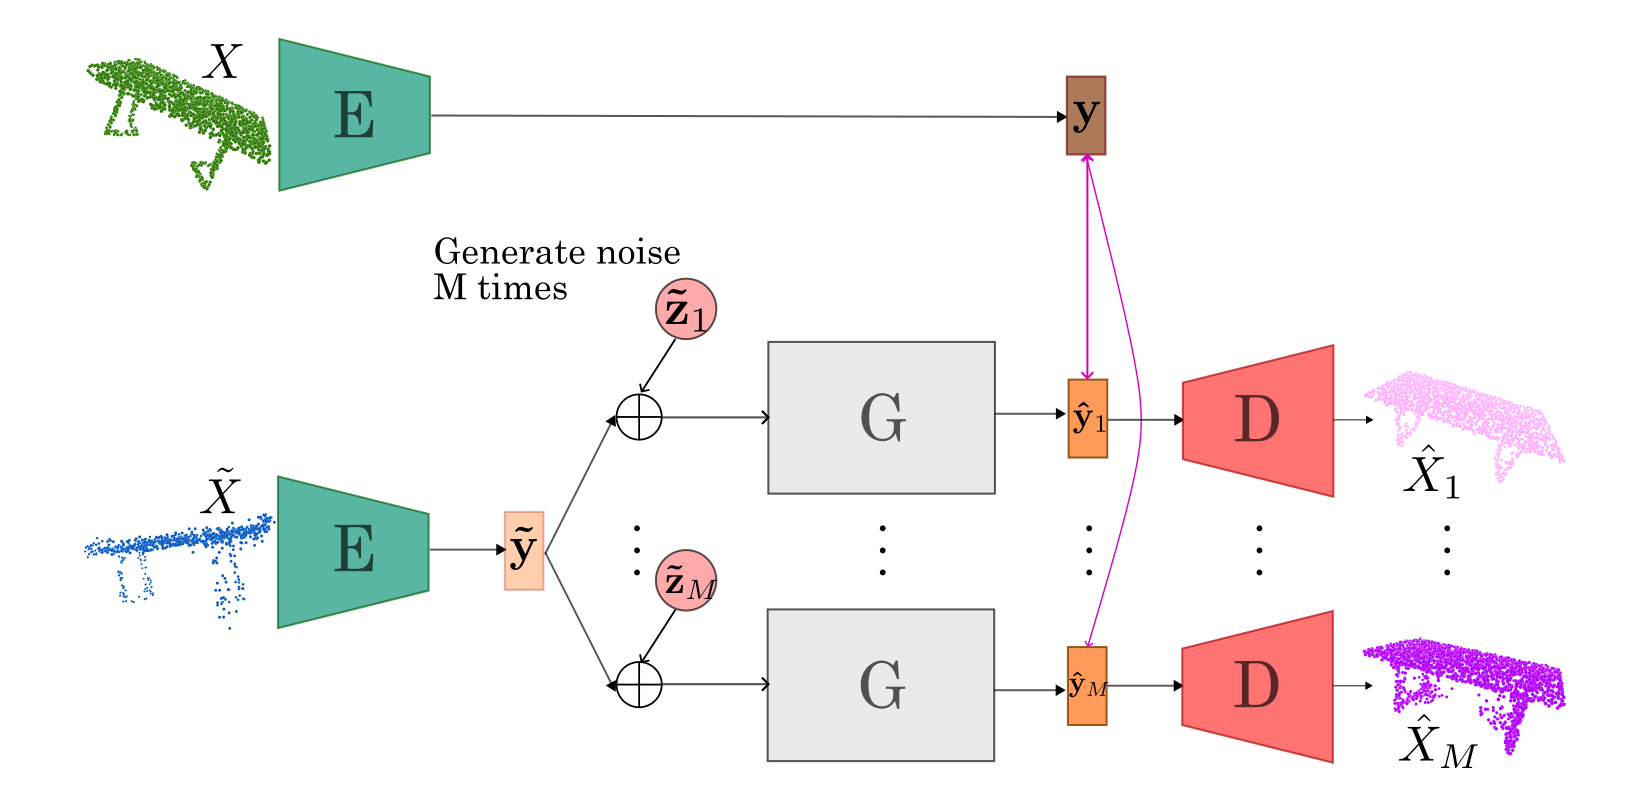
\includegraphics[width=\linewidth]{figures/implicit_gen_network.png}
          \end{center}
          \caption{Network for point cloud completion uncertainty quantification using conditional implicit generation. During inference, noise is sampled from a standard Gaussian distribution multiple times, and encodings are generated based on the different noises.}\label{fig:implicit_net}
        \end{figure}
        Another possible method to generate non-deterministic predictions from an input is to add random noise to the input before passing it to the generator. Eq.~\ref{IGM} can be reformulated for conditional implicit generative models as:
        \begin{equation}\label{IGM}
            \mathbf{\tilde{z}} \sim q(\mathbf{z}), \quad \mathbf{\hat{y}} =  \mathcal{G}_\theta(\mathbf{\tilde{z}}; \mathbf{\tilde{y}})
        \end{equation}
        where $\mathcal{G}$ is specified by an NN with parameters $\theta$. With different $\mathbf{\tilde{z}}$ different $\mathbf{\hat{y}}$ corresponding to different complete shape for a fixed $\mathbf{\tilde{y}}$ can be generated (see Figure~\ref{fig:implicit_net}).

    \subsection{Training Procedure}
        \subsubsection{Learning encoding for point clouds}
        \begin{figure}[htb]
          \begin{center}
          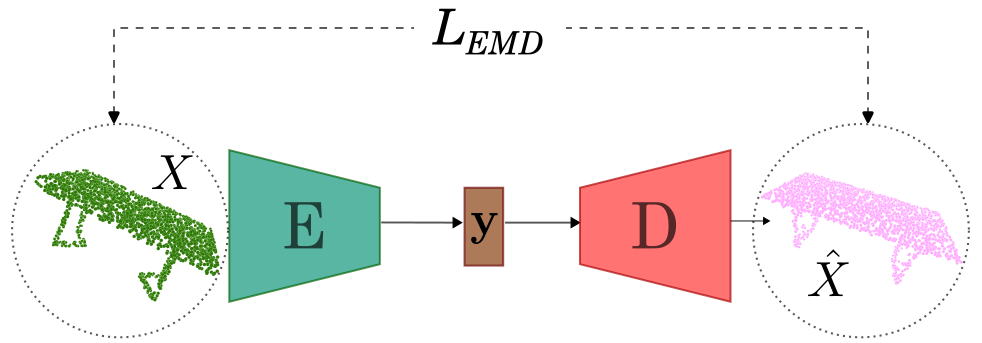
\includegraphics[width=\linewidth]{figures/emd_ae.png}
          \end{center}
          \caption{Training autoencoder by minimizing Earth mover's distance.}\label{fig:emd_ae}
        \end{figure}
        One can learn to produce the encoding of a given point cloud by training an autoencoder, which encodes the given input to a lower-dimensional feature vector called a latent code or an encoding, and subsequently decodes the encoding to reconstruct the original input. The autoencoder can be a standard autoencoder (AE), a variational autoencoder (VAE), or a vector-quantized variational autoencoder (VQ-VAE), depending on a deliberate choice. The autoencoder is trained for a reconstruction task on a point cloud dataset for both partial and complete shapes.
        \newline
        
        For instances of ground truth point cloud $X=\left\{\mathbf{x}_{i} \in \mathbb{R}^{3}\right\}_{i=1}^{N_C}$ from the dataset of complete clouds $\mathbf{X_C} \in \mathbb{R}^{N \times N_C \times 3}$, an encoder-decoder network is trained to learn an encoder mapping $\mathcal{E}: \mathbb{R}^{N_C \times 3} \rightarrow \mathbb{R}^{\ell}$ that takes the concatenation of coordinates of the $N_C$ points in complete cloud as input and produces an encoding in the latent space with dimension $\ell$ along with a decoder mapping $\mathcal{D}: \mathbb{R}^{\ell} \rightarrow \mathbb{R}^{N_C \times 3}$ that inverts the encoding back to a reconstructed point cloud with $N_C$ points as before. The autoencoder is trained using a reconstruction loss based on Earth Mover's Distance (EMD). The reconstruction loss for a point cloud $X$ is denoted as:
        \begin{equation}\label{emd_loss}
            L_{EMD} = d_{EMD}\left(X, \mathcal{D}(\mathcal{E}(X))\right),
        \end{equation}
        where $d_{EMD}\left(X, \mathcal{D}(\mathcal{E}(X))\right)$ denotes the Earth Mover's Distance between the input cloud and the reconstructed cloud (see Figure~\ref{fig:emd_ae}). Then the objective function for training the autoencoder can be computed as:
        \begin{equation}\label{emd_obj}
            \mathcal{L}_{EMD} = \mathbb{E}_{X \sim p(X)} \left[d_{EMD}\left(X, \mathcal{D}(\mathcal{E}(X))\right)\right]
        \end{equation}
        where $p(X)$ denotes a distribution over the space of complete clouds from which we sample.
        \newline
        
        The encoding produced by the encoder provides a ready-made representation, which implicitly captures the shape manifold for a point cloud, to be used in downstream tasks. So, once training is done, the network parameters are fixed while using the encoder and decoder in any subsequent network. As for the instances of point cloud $\tilde{X}=\left\{\mathbf{\tilde{x}}_{i} \in \mathbb{R}^{3}\right\}_{i=1}^{N_P}$ from the dataset of partial clouds $\mathbf{X_P} \in \mathbb{R}^{N \times N_P \times 3}$, a separate auto-encoder is not trained. Rather, the partial cloud is directly passed to the autoencoder trained with complete clouds to produce encoding in the latent space, which is known to work better for downstream applications. To do that, some points from the partial point cloud can be copied to match the number of points in the complete cloud before feeding it to the encoder. Alternatively, an encoder invariant of point set size, similar to PointNet~\cite{PointNet}, can be used.


        \subsubsection{Learning to generate multiple point clouds}
        \begin{figure}[htb]
          \begin{center}
          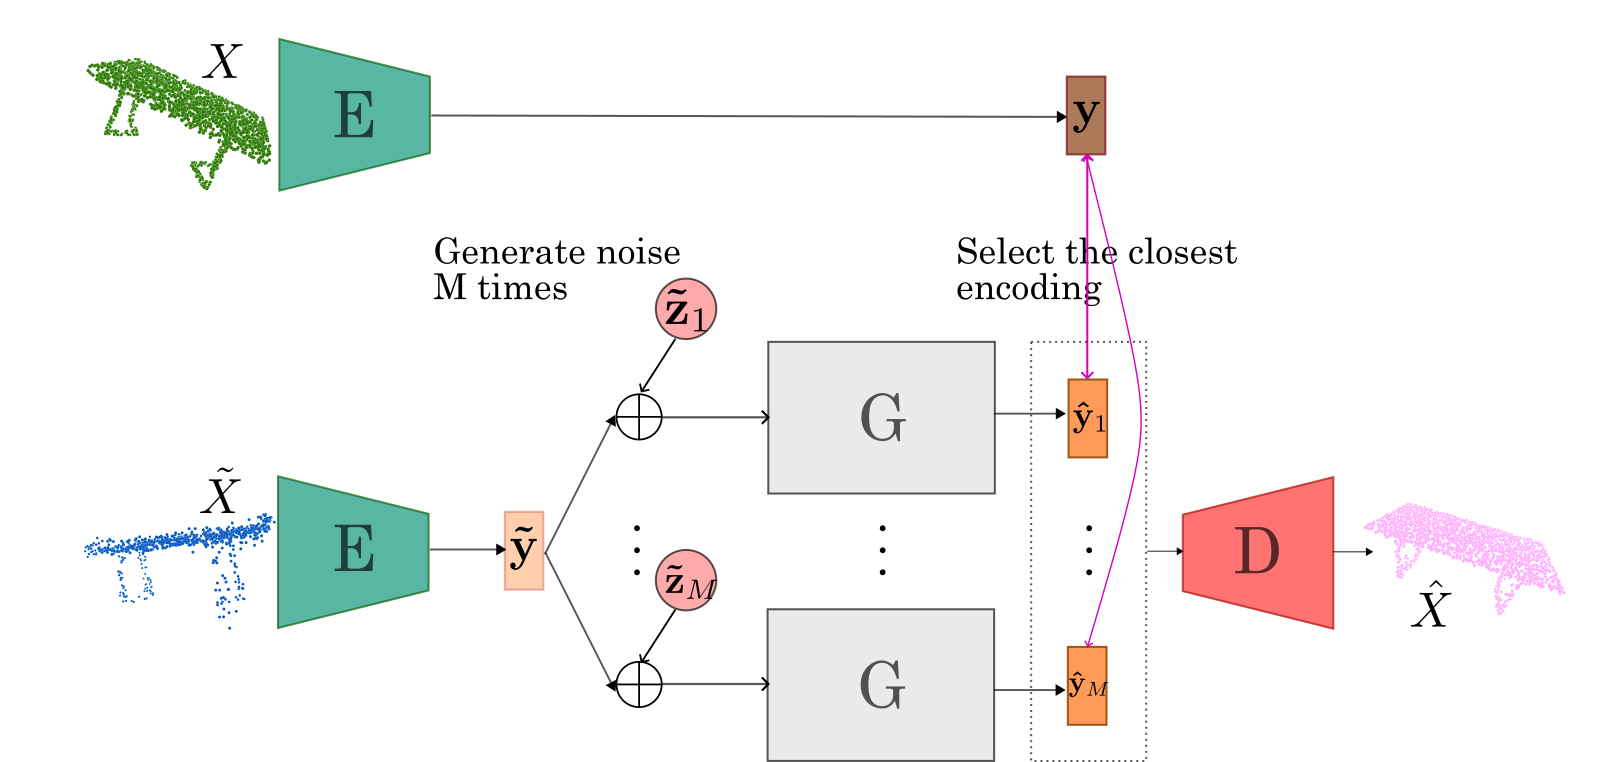
\includegraphics[width=\linewidth]{figures/implicit_gen_network_imle.png}
          \end{center}
          \caption{Training network for point cloud completion uncertainty quantification using conditional implicit maximum likelihood estimation. During training, not all encodings generated from G are compared with the complete cloud encoding $\mathbf{y}$. Only the closest encoding is selected during training.}\label{fig:imle}
        \end{figure}
        Training differs according to the method selected for uncertainty quantification (more precisely, methods for inducing randomness) to produce different complete shapes. If dropout or DropConnect is used, the training procedure becomes quite straightforward. The same general structure for point completion depicted in Figure~\ref{fig:gen_net} is followed with the generator $G$ using dropout or DropConnect during training. If an ensemble of generators with $M$ models is used, then each generator needs to be trained individually, resulting in $M$ different training sequences similar to the procedure shown in Figure~\ref{fig:ens_net}. In this case, the inference and training follow the same pattern. 
        \newline
        
        Finally, for the implicit generation, one learns to produce different complete shapes for a fixed partial input based on the noise injected into the generator. Since only one possible target shape is available for each partial shape, it needs to be trained differently from just computing the loss based on the one-to-one correspondence. Otherwise, any addition of noise will be rendered inconsequential, resulting in mode collapse and similar completion results. Note that this is not an issue for dropout or ensemble models. With dropping out, the uncertainty is inherently induced through the different selection of weights or nodes during training. For the ensemble, all the models are trained separately. 
        \\
        For training conditional implicit generative models, conditional Generative Adversarial Networks (GANs) had been the go-to approach for a long period. However, due to several drawbacks, such as mode collapse, the popularity of GANs has dwindled, with new approaches overturning the downsides of using GANs. One such method, called Implicit Maximum Likelihood Estimation (IMLE), was introduced by~\cite{IMLE}.~\cite{PCCIMLE} already applied the same idea for point cloud completion, which is adopted here. The authors of~\cite{PCCIMLE} demonstrated that using conditional IMLE to train implicit generation yields more diverse completion results, thereby resolving the mode collapse issue. Here, rather than comparing all the generated encodings ($\{\mathbf{\hat{y}}_i\}_{i=1}^M$) with the encoding of the complete shape $\mathbf{y}$, only the one closest to $\mathbf{y}$ is chosen as shown in Figure~\ref{fig:imle}. This way, not every generated encoding is close to the encoding of the complete cloud, but every complete shape encoding has one generated encoding trained to be close in the latent space. This ensures that mode collapse does not happen, and every complete shape in the training data has at least one similar shape generated.

        \begin{figure}[htb]
          \begin{center}
          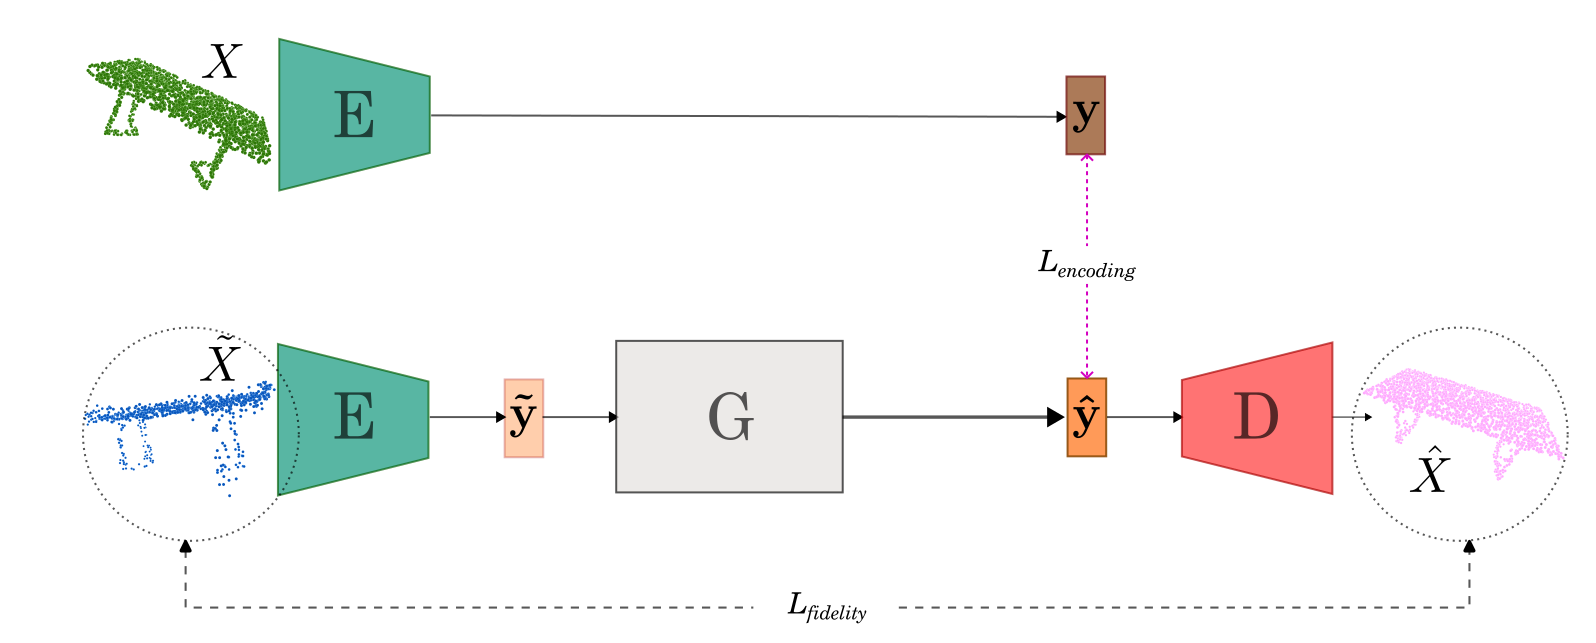
\includegraphics[width=\linewidth]{figures/losses_main_network.png}
          \end{center}
          \caption{Losses for training the main network for point cloud completion with uncertainty.}\label{fig:losses_main}
        \end{figure}
        To train the network (generator), the loss functions that are to be minimized need to be specified (see Figure~\ref{fig:losses_main}). As discussed above, the parameters of the encoder-decoder network trained for reconstruction are fixed. For a ground truth point cloud $X=\left\{\mathbf{x}_{i} \in \mathbb{R}^{3}\right\}_{i=1}^{N_C}$ from the dataset of complete clouds $\mathbf{X_C} \in \mathbb{R}^{N \times N_C \times 3}$, it is fed to the encoder network to get its encoding $\mathbf{y}$. Similarly, the corresponding point cloud $\tilde{X}=\left\{\mathbf{\tilde{x}}_{i} \in \mathbb{R}^{3}\right\}_{i=1}^{N_P}$ from the dataset of partial clouds $\mathbf{X_P} \in \mathbb{R}^{N \times N_P \times 3}$ is passed to the encoder to obtain its encoding $\mathbf{\tilde{y}}$. Now, $\mathbf{\tilde{y}}$ is passed through the generator according to the selected architecture among the ones explained above. For dropout or DropConnect, only one encoding $\mathbf{\hat{y}}$ is generated and compared with $\mathbf{y}$. Otherwise, $M$ encodings $\{\mathbf{\hat{y}}_i\}_{i=1}^M$ are generated corresponding to the $i$-th model in the ensemble or $i$-th noise sampled for implicit generation. In the ensemble method, each of $\{\mathbf{\hat{y}}_i\}_{i=1}^M$ is compared to $\mathbf{y}$. In implicit generation, the proposed IMLE method is followed, and the encoding in $\{\mathbf{\hat{y}}_i\}_{i=1}^M$ closest to $\mathbf{y}$ with $\mathbf{y}$ is compared. The corresponding loss function between two encodings is denoted as:
        \begin{equation}\label{latent_loss}
            L_{encoding}(\mathbf{y}, \mathbf{\hat{y}}) = \left\|\mathbf{y} - \mathbf{\hat{y}}\right\|_2^2,
        \end{equation}
        which is the Euclidean distance between the two encodings. 
        \\
        One also needs to ensure that the complete shapes generated are faithful to the partial shape. To maintain the fidelity of the completion results produced from the encodings output by the generator, the unidirectional Hausdorff distance between the partial cloud and the generated complete cloud is used. The corresponding loss is denoted as:
        \begin{equation}\label{fidelity_loss}
            L_{fidelity}(\tilde{X}, \hat{X}) = \max_{\mathbf{\tilde{x}}_{i} \in \tilde{X}} \min_{\mathbf{\hat{x}}_{j} \in \hat{X}} \left\|\mathbf{\tilde{x}}_{i}-\mathbf{\hat{x}}_{j}\right\|_2,
        \end{equation}
        where $\hat{X}=\left\{\mathbf{\hat{x}}_{j} \in \mathbb{R}^{3}\right\}_{j=1}^{N_C}$ is the set of generated point clouds. So the overall objective for training the network is:
        \begin{equation}\label{gen_obj}
            \begin{aligned}
                \mathcal{L}_{pcc} = \mathbb{E}_{X, \tilde{X} \sim p(X, \tilde{X})} \left[\lambda_{encoding} L_{encoding}\left(\mathcal{E}(X), \mathcal{G}_\theta(\mathcal{E}(\tilde{X}))\right)\right \\
                + \left\lambda_{fidelity} L_{fidelity}(\tilde{X}, \mathcal{D}\left(\mathcal{G}_\theta(\mathcal{E}(\tilde{X})))\right)\right]
            \end{aligned},
        \end{equation}
        where $\mathcal{E}$ is the encoder mapping, $\mathcal{D}$ is the decoder mapping, and $\mathcal{G}_\theta$ is the generator mapping by the NN parametrized by $\theta$. For IMLE, the above objective changes to:
        \begin{equation}\label{gen_obj_imle}
            \begin{aligned}
                \mathcal{L}_{pcc}^{imle} = \mathbb{E}_{X, \tilde{X} \sim p(X, \tilde{X}), \mathbf{Z}} \left[\lambda_{encoding} \min_{i=1, \ldots, M} L_{encoding}\left(\mathcal{E}(X), \mathcal{G}_\theta(\mathcal{E}(\tilde{X}), \mathbf{\tilde{z}}_i)\right)\right \\
                + \left\lambda_{fidelity} L_{fidelity}(\tilde{X}, \mathcal{D}\left(\mathcal{G}_\theta(\mathcal{E}(\tilde{X})))\right)\right]
            \end{aligned},
        \end{equation}
        where $\mathbf{Z} = (\mathbf{\tilde{z}}_1, \ldots, \mathbf{\tilde{z}}_M)^T$ such that $\mathbf{\tilde{z}}_i \sim \mathcal{N}(0, I_z) \forall i=\{1, \ldots, M\}$ with noise dimension $z$ and hyperparameter M.


    \subsection{Uncertainty Map Computation with Matching}
    \begin{figure}[htb]
      \begin{center}
      \includegraphics[width=\linewidth]{figures/matching_edited.png}
      \end{center}
      \caption{Linear assignment for matching between a pair of generated point clouds. For each point in the green cloud, the closest point in the purple cloud is located based on some cost function. Notice that the representative indices of the matched points are different in the respective tensors of the generated clouds.}\label{fig:matching}
    \end{figure}
    Rather than naively computing the index-wise mean and variance of the 3D coordinates of the generated complete clouds, the point sets can be matched between themselves as one-to-one mappings of points. Such matchings between two point clouds can be computed using a minimum-weight matching or linear assignment with an appropriate cost of matching a point from one cloud to a point in another. Hungarian matching algorithm~\cite{Hungarian} or a modified version of Jonker-Volgenant algorithm~\cite{RectAssign} were applied to perform the matching between clouds. Euclidean distance between points was used as the cost function. One of the generated complete clouds was selected at random, and one-to-one mappings with points in the remaining complete clouds were identified. The resulting matching was then used to compute the mean and variance estimations of the predicted complete point cloud.


\section{Empirical Uncertainty Quantification for Implicit Neural Representation}\label{euqinr}
In this section, a solution to the Problems~\ref{SingleCloud} and~\ref{DataCloud} is proposed by predicting uncertain implicit representations for the given input cloud. An implicit representation is a function $f: \mathbb{R}^{3} \mapsto \mathbb{R}$ such that the zero level set of $f$ precisely approximates the surface on the 3D shape denoted by $\mathcal{S}$ :
\begin{equation}
\mathcal{S} \approx \left\{\mathbf{x} \in \mathbb{R}^{3} \mid f(\mathbf{x})=0\right\}
\end{equation}
\newline

Instead of directly computing the probabilistic estimate of the underlying surface, one can first generate multiple possible implicit representations $\{f_i: \mathbb{R}^3 \mapsto \mathbb{R}\}_{i=1}^M$ from the input and then empirically estimate the surface along with the associated uncertainty from the different implicit representations. From previous works, it is known that the neural implicit function $f$ usually approximates the (un-)signed distance function (UDF/SDF), which maps any point in space to the distance to its closest point on the surface. For a function $f$ to be a distance function corresponding to a given point cloud $X=\left\{\mathbf{x}_{i} \in \mathbb{R}^{3}\right\}_{i=1}^{N_C}$, it needs to satisfy some conditions or constraints as enumerated below~\cite{DiGS, NeuralHessian}:
\begin{enumerate}
    \item Dirichlet condition or manifold constraint: the observed points in the point cloud lie on the surface of the object, $f(\mathbf{x})=0$ for $\mathbf{x} \in X$.
    \item Eikonal constraint: all points have a unit gradient, $\|\nabla f\|=1$.
    \item Neumann condition or normal constraint:  the gradients of points match the ground truth normal field if normal information is available, $\nabla f=\mathcal{N}$, where $\mathcal{N}$ is the normal field.
    \item Non-manifold constraint: non-manifold points (points not on the surface) have the same value as their ground truth SDF or UDF if the distance values are available.
    \item Non-manifold penalisation constraint: non-manifold points have non-zero implicit function values.
\end{enumerate}
Out of the above constraints, while the manifold constraint and one of the Eikonal constraint or the Non-manifold constraint are necessary, the rest are mostly used as additional criteria to enhance the results~\cite{DiGS}. Since only unoriented point clouds without normal information or SDF/UDF values are available for supervision, normal constraint and non-manifold constraint cannot be used. The remaining 3 constraints for a given point cloud $X=\left\{\mathbf{x}_{i} \in \mathbb{R}^{3}\right\}_{i=1}^{N_C}$ are used, which give rise to the following loss functions:
\begin{equation}\label{manifold_sdf}
    \mathcal{L}_{\text {manifold }}=\int_{X}\|f(x)\|_{1} d x \approx \frac{1}{N_C}\sum_{i=1}^{N_C}\|f(\mathbf{x}_i)\|_1
\end{equation}
\begin{equation}\label{non_manifold_sdf}
    \mathcal{L}_{\text {non-manifold }}=\int_{\underline{X}} \exp \left(-\alpha\|f(x)\|_{1}\right) d x \approx \frac{1}{N_C}\sum_{i=1}^{N_C} \exp \left(-\alpha\|f(\underline{\mathbf{x}_i})\|_1\right),
\end{equation}
where $\underline{X}=\left\{\underline{\mathbf{x}_i} \in \mathbb{R}^{3}\right\}_{i=1}^{N_C}$ is the set of points off the surface and $\alpha>>1$.
\begin{equation}\label{Eikonal}
     \begin{aligned}
         \mathcal{L}_{\text {Eikonal }}=\int_{X \cup \underline{X}} \| \| \nabla f(x)\left\|_{2}-1\right\|_{1} d x \\
         \approx \frac{1}{N_C}\sum_{i=1}^{N_C} \left(\| \| \nabla f(\mathbf{x}_i)\left\|_{2}-1\right\|_{1} + \| \| \nabla f(\underline{\mathbf{x}_i})\left\|_{2}-1\right\|_{1} \right).
     \end{aligned}
\end{equation}
The combined objective function can then be computed as:
\begin{equation}\label{inr_loss1}
    \mathcal{L}_{inr}= \lambda_{\text {manifold }} \mathcal{L}_{\text {manifold }}+\lambda_{\text {non-manifold }} \mathcal{L}_{\text {non-manifold }}+ \lambda_{\text {Eikonal }} \mathcal{L}_{\text {Eikonal }}
\end{equation}
where $\lambda_{\text {manifold }}, \lambda_{\text {non-manifold }}, \lambda_{\text {Eikonal }}$ are the corresponding regularization weights.
\newline

However, optimizing the above objective is not sufficient to produce optimal results, as demonstrated by~\cite{DiGS, NeuralHessian}. As discussed in section~\ref{INR-old}, several works have tried to solve this issue by introducing an additional loss depending upon the intended geometric effect. Since only unoriented point clouds are available as inputs, the loss based on the Hessian matrix defined in~\cite{NeuralHessian} was employed. The loss function associated with the Hessian matrix can be computed as:
\begin{equation}\label{Hessian1}
    \mathcal{L}_{\text{Hessian }} = \int_{\circled{$X$}} \left|Det(\mathbf{H}_f(x))\right| d x \approx \frac{1}{N_C}\sum_{i=1}^{N_C} \left|Det\left(\mathbf{H}_f\left(\circled{$\mathbf{x}_i$}\right)\right)\right|,
\end{equation}
where $\circled{$X$}=\left\{\circled{$\mathbf{x}_i$} \in \mathbb{R}^{3}\right\}_{i=1}^{N_C}$ is the set of points close to the surface and $Det(\cdot)$ refers to the determinant of the matrix. So the overall objective function now becomes:
\begin{equation}\label{Hessian2}
    \begin{aligned}
        \mathcal{L}_{inr}= \lambda_{\text {manifold }} \mathcal{L}_{\text {manifold }}+\lambda_{\text {non-manifold }} \mathcal{L}_{\text {non-manifold }}+ \lambda_{\text {Eikonal }} \mathcal{L}_{\text {Eikonal }}
        \\
        +\lambda_{\text{Hessian }} \tau \mathcal{L}_{\text{Hessian }},
    \end{aligned}
\end{equation}
where $\tau$ is the annealing factor defined in~\cite{NeuralHessian}. Now that the objective is defined, the method for introducing randomness in implicit function prediction to calculate uncertainty can be discussed.


    \subsection{Predicting Implicit Representation with Randomness}
    \begin{figure}[htb]
      \begin{center}
      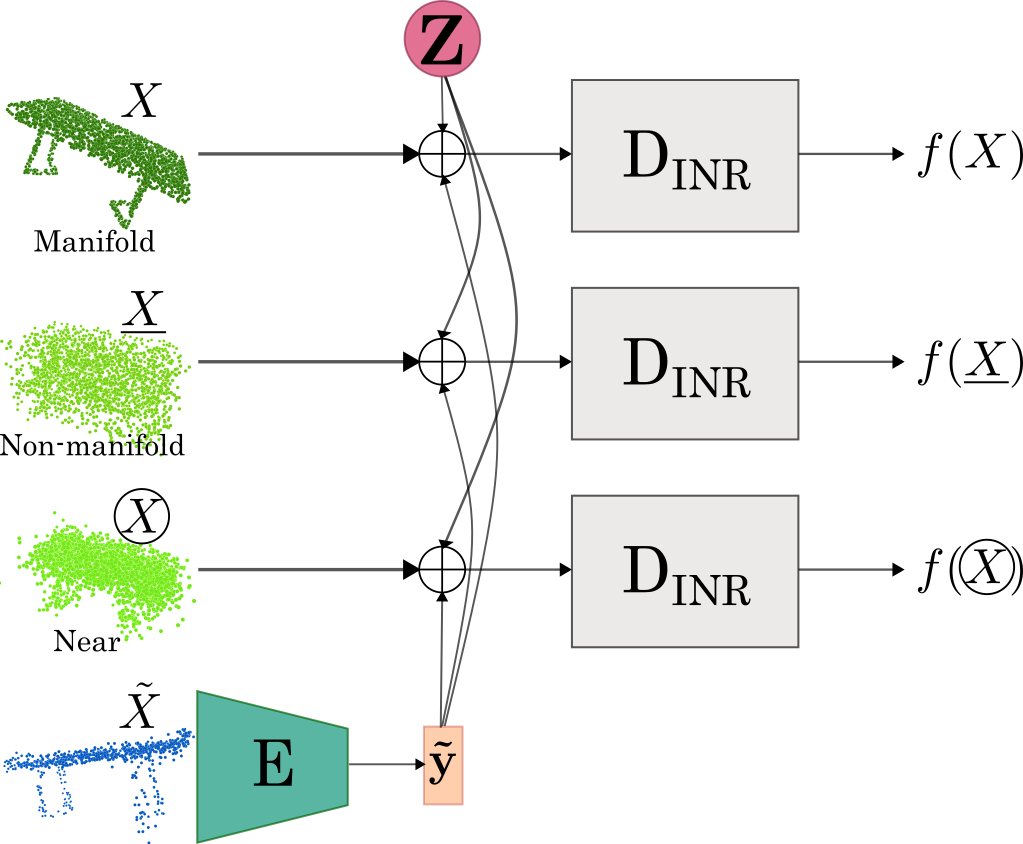
\includegraphics[width=\linewidth]{figures/inr_network.png}
      \end{center}
      \caption{General structure of network used for training implicit function with randomness. During training, the partial cloud $\tilde{X}$ is input to the encoder E to output the encoding $\mathbf{\tilde{y}}$. Manifold, non-manifold, and near points conditioned on $\mathbf{\tilde{y}}$ and noises are fed to the decoder D$_{\text{INR}}$ to predict the implicit function corresponding to the noise.}\label{fig:inr_net}
    \end{figure}
    Randomness can be introduced into the network architecture that approximates the implicit function using any of the uncertainty quantification methods discussed in Section~\ref {back_uqdl}. For Problem~\ref{SingleCloud}, the network structure is straightforward. Existing shape space learning architectures for point clouds can be used, such as a standard or variational autoencoder, with the decoder output being the implicit representation instead of a reconstructed cloud. On the other hand, for Problem~\ref{DataCloud}, partial and complete cloud pairs are available during training, but only the partial cloud is available for inference. Therefore, an information disparity exists between the training and inference processes if the implicit representation is directly learned from complete clouds in the shape space. To gain a clearer understanding of the information lost without the complete cloud, the sampling procedure used to learn the implicit function is described first.
    \newline
    
    To sample points not on the surface (points in the set $\underline{X}$), a bounding box around the point cloud was found, and points within that box were sampled uniformly. Considering most points inside the box are off the surface, sampling a point on the surface is highly unlikely. To sample points close to the surface (points in the set \circled{$X$}), the sampling used in~\cite{IGR, SALD, NeuralHessian} was emulated. For each point $\mathbf{x}_i$ on the surface, the distance to the $k$-th nearest point ($k=50$ used by previous methods) was found and denoted as $d$. Then one point from the Gaussian distribution $\mathcal{N}(\mathbf{x}_i, d^2I)$ was sampled to find a point close to the surface. One can observe that while sampling of non-manifold points is not affected by the unavailability of a complete cloud, sampling of points close to the surface differs. So, using points close to the surface was avoided during inference. Additionally, since only the partial point cloud is available at test time, the encoding of the complete cloud cannot be used during learning. With all that in mind, the architecture depicted in Figure~\ref{fig:inr_net} is proposed.
    \newline
    
    The complete point cloud $X$ is considered as the points lying on the surface (manifold points). The non-manifold and near point sets $\underline{X}$ and \circled{$X$} were sampled as explained. The partial cloud $\tilde{X}$ is fed to the encoder E to get the encoding $\mathbf{\tilde{y}}$. Parallelly, multiple noises $\mathbf{Z} = (\mathbf{\tilde{z}}_1, \ldots, \mathbf{\tilde{z}}_M)^T$ were sampled such that $\mathbf{\tilde{z}}_i \sim \mathcal{N}(0, I_z) \forall i=\{1, \ldots, M\}$ with noise dimension $z$ and hyperparameter $M$. The manifold, non-manifold, and near points conditioned on the encoding $\mathbf{\tilde{y}}$ and noises are then passed to the decoder D$_{\text{INR}}$ to predict the implicit function corresponding to each noise. If, during training, the objective for the implicit function predicted for each noise is minimized, the issue of mode collapse might appear. This will lead to a lack of diversity in predicted implicit functions. Therefore, during training, only the noise leading to the implicit function with minimum manifold loss ($\mathcal{L}_{\text {manifold }}$) was chosen for computing the rest of the objective function and performing backpropagation. During inference, different implicit functions based on different noises were predicted, and the mean and variance at any point were empirically estimated based on these predicted functions to obtain our reconstructed surface with associated uncertainty.
    \newline
    
    The learned encoding also needs to be regularized for better shape space learning using autoencoder architectures. For a standard autoencoder, the regularization loss can be computed as:
    \begin{equation}\label{reg_latent}
        \mathcal{L}_{\text {reg }} = \left\|\mathcal{E}(\tilde{X})\right\|_2^2,
    \end{equation}
    where $\mathcal{E}$ is the encoder mapping. For a variational autoencoder, the  regularization loss can be computed as (similar to~\cite{SAL}):
    \begin{equation}\label{reg_latent}
        \mathcal{L}_{\text {reg }} = \left\|\mu\left(\mathcal{E}(\tilde{X})\right)\right\|_1 +\left\|diag(\Sigma\left(\mathcal{E}(\tilde{X})\right)\right\|_1,
    \end{equation}
    where $diag$ is the diagonal matrix, $\mu$ denotes the latent prediction (mean function) and $\Sigma$ refers to the covariance matrix for latent prediction. Such regularization enforces the latent means to be near zero and the covariances to be close to identity matrices. With the addition of the regularization term, the overall objective function becomes:
    \begin{equation}\label{Hessian3}
        \begin{aligned}
            \mathcal{L}_{inr}= \lambda_{\text {manifold }} \mathcal{L}_{\text {manifold }}+\lambda_{\text {non-manifold }} \mathcal{L}_{\text {non-manifold }}+ \lambda_{\text {Eikonal }} \mathcal{L}_{\text {Eikonal }}
            \\
            + \lambda_{\text{Hessian }} \tau \mathcal{L}_{\text{Hessian }} + \lambda_{\text {reg }} \mathcal{L}_{\text {reg }},
        \end{aligned}
    \end{equation}

    

\section{Gaussian Process-based Uncertainty Quantification for 3D Shapes}\label{gpuq}
In this section, the Problems~\ref{SingleCloud} and~\ref{DataCloud} are tackled by describing an uncertain implicit representation for the given input cloud by a Gaussian process. Several existing works (see section~\ref{Stoch-old}) follow a similar approach for a single point cloud (Problem~\ref{SingleCloud}). Therefore, the focus in this thesis will be solely on methods to solve Problem~\ref{DataCloud}.

\begin{figure}[htb]
      \begin{center}
      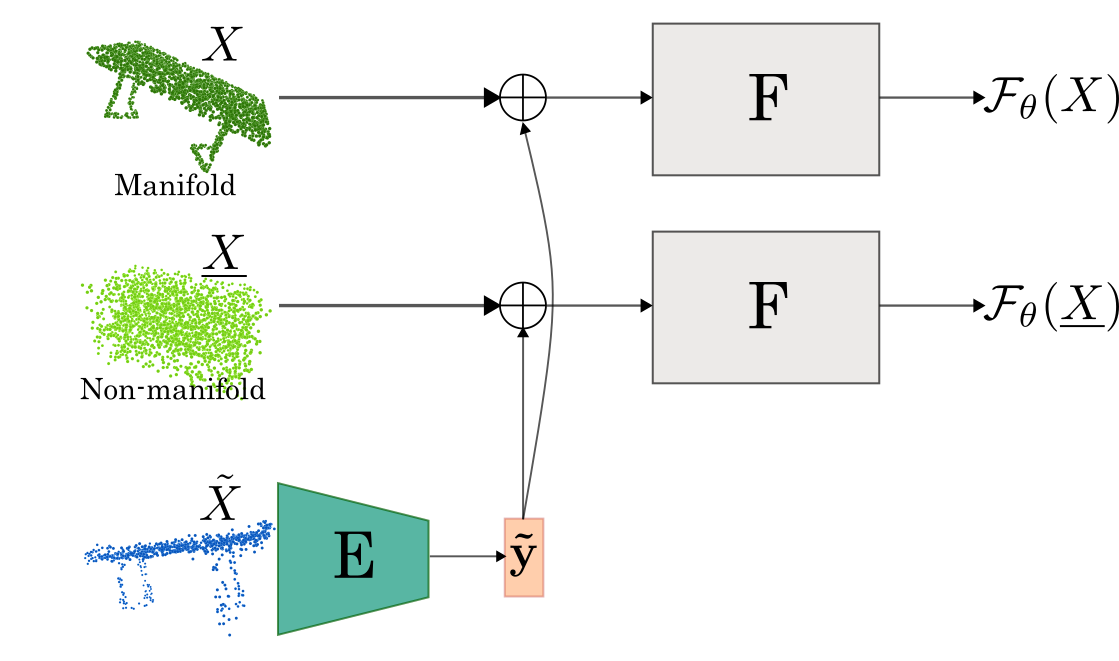
\includegraphics[width=\linewidth]{figures/gpr_network.png}
      \end{center}
      \caption{General structure of network used for learning feature mapping. During training, the partial cloud $\tilde{X}$ is input to the encoder E to output the encoding $\mathbf{\tilde{y}}$. Manifold and non-manifold points conditioned on $\mathbf{\tilde{y}}$ are fed to the neural network F to predict the output of feature mapping $\mathcal{F}_\theta$.}\label{fig:gpr_net}
\end{figure}

It is known that the surface is represented by the zero level set of the implicit function $f: \mathbb{R}^{3} \mapsto \mathbb{R}$. Therefore, for all non-manifold points $\mathbf{x} \in \mathbb{R}^{3}$, $f(\mathbf{x}) \neq 0$. For a given partial and complete cloud pair, a function needs to be learnt that outputs zero for points on the surface and non-zero values otherwise when conditioned on the partial point cloud. Similar to the method described in section~\ref{euqinr}, the partial cloud $\tilde{X}$ is encoded to get the latent code $\mathbf{\tilde{y}}$. The complete point cloud $X$ is considered as the set of points lying on the surface (manifold points). As in section~\ref{euqinr}, non-manifold points are sampled by finding a bounding box around the complete cloud and uniformly sampling points within that box. Points sampled close to the complete cloud are removed.  Now, the Gaussian process posterior mean for each manifold point conditioned on $\mathbf{\tilde{y}}$ should be zero, and for non-manifold points conditioned on $\mathbf{\tilde{y}}$ should be farther from zero.


    \subsection{Challenges of Modeling a Gaussian Process}
    Several important aspects need to be considered in the setting explained above before modeling the implicit representation by a Gaussian process. A brief overview of the challenges, modifications, and possible solutions is discussed below.

        \subsubsection{Lack of Non-zero Supervision}
        An important aspect to consider is that only the unoriented point clouds are observed, meaning only samples $\mathbf{x}$ for which $f_{\mathbf{\tilde{y}}}(\mathbf{x}) = 0$ are available where $f_{\mathbf{\tilde{y}}}$ denotes the implicit function $f$ conditioned on the encoding $\mathbf{\tilde{y}}$ of partial cloud. Although points off the surface were sampled, their ground truth function values were not known. This makes the problem quite challenging, as without supervision from non-zero-valued samples, the Gaussian process regression with zero-mean prior fails to predict non-zero values for points not on the surface, leading to multiple ghost geometries. This is also evident from Eq.~\ref{GPPosterior0} as the posterior mean becomes zero if $\mathbf{Y}=\mathbf{0}$. 
        \newline

        One simple workaround for the above issue can be found in the formulation of the posterior distribution of a GP given in Eq~\ref{GPPosterior}. One can simply consider a prior mean greater than zero (e.g., $m(\mathbf{x})=1$) to reflect the fact that more often than not, any point in space (or even in a bounding box around the point cloud) will not lie on the surface. Then, with conditioning on the observed points on the surface having zero values, the corresponding implicit surface becomes evident, and consequently, the posterior distribution estimates the 3D shape. A simple mathematical explanation of the effect of non-zero bias in prior mean is given in Appendix~\ref{ch:nonzerogp}.

        \subsubsection{Stationary Covariance Function}
        As a Gaussian process modeling spatial information, certain important properties need to be restricted when considering the covariance function. As noticed in previous works, the covariance functions employed were isotropic, meaning they are stationary and symmetric. The covariance function is stationary if it depends only on the difference or relative distance between the input points, rather than on their individual positions. Mathematically, $k(\mathbf{x_1}, \mathbf{x_2}) = k(\mathbf{x_1} - \mathbf{x_2}) = k(\mathbf{r})$. The covariance function is symmetric if $k(\mathbf{x_1}, \mathbf{x_2}) = k(\mathbf{x_2}, \mathbf{x_1})$. Combining both, the covariance function is isotropic if it depends only on the absolute relative distance between the input points, i.e., if $k(\mathbf{x_1}, \mathbf{x_2}) = k(|\mathbf{x_1} - \mathbf{x_2}|) = k(|\mathbf{r}|)$.
        \\
        The necessity of the stationary property is evident from the fact that the distance function or implicit function values are similar for points close to each other, and the distance between points in space inherently imposes that similarity. Therefore, the covariance functions experimented with also maintained the stationary property. But this poses a challenge to directly model a conditional Gaussian process. As discussed, the implicit function is modeled conditioned on the partial cloud encoding $\mathbf{\tilde{y}}$. Now, if the encoding is directly concatenated with the 3-D coordinates of the points as inputs to the Gaussian process, the effect of conditioning will be rendered useless in case of a stationary covariance function based on relative distance. Mathematically, it can be shown that $(\mathbf{x_1}; \mathbf{\tilde{y}}) - (\mathbf{x_2}; \mathbf{\tilde{y}}) = (\mathbf{x_1}-\mathbf{x_2}; \mathbf{0})$ and therefore, $k((\mathbf{x_1}; \mathbf{\tilde{y}}),  (\mathbf{x_2}; \mathbf{\tilde{y}})) = k((\mathbf{x_1}-\mathbf{x_2}; \mathbf{0})) = k(\mathbf{x_1}-\mathbf{x_2})$ since the dimensions with zero values do not contribute to the kernel computation.
        \newline

        As a result, an alternative approach is needed to model the kernel or covariance function. Following the idea introduced by the authors of~\cite{DKL}, the input coordinates conditioned on the encoding $\mathbf{\tilde{y}}$ are mapped to a new embedding space of dimension $d$ using a feature mapping $\mathcal{F}_\theta: \mathbb{R}^{3+\ell} \mapsto \mathbb{R}^d$ where $\ell$ is the dimension of the encoding and $\mathcal{F}_\theta$ is a non-linear mapping modeled by a deep NN parametrized by $\theta$. This way, the base kernel is transformed as:
        \begin{equation}\label{dkl}
            k((\mathbf{x_1}; \mathbf{\tilde{y}}),  (\mathbf{x_2}; \mathbf{\tilde{y}})) \mapsto k(\mathcal{F}_\theta(\mathbf{x_1}; \mathbf{\tilde{y}}),  \mathcal{F}_\theta(\mathbf{x_2}; \mathbf{\tilde{y}})).
        \end{equation}
        For the base kernel, any standard stationary kernel can be chosen. A popular choice is the radial basis function (RBF) kernel given by:
        \begin{equation}
            k_{\text{RBF}}(\mathbf{x_1},  \mathbf{x_2}) = \exp \left(-\frac{\|\mathbf{x_1}-\mathbf{x_2}\|^2}{2l^2}\right),
        \end{equation}
        where $l$ is the length scale of the kernel. With the above formulation set up, an objective function needs to be decided now to learn the feature mapping NN.


        \subsection{Objective Function for Learning the Feature Map}
            \subsubsection{Log-Likelihood}
            During training, both partial and complete clouds are available, but only the partial cloud is provided for inference. So, the input information is inconsistent between the
            training and inference processes if the complete clouds are directly used to model the Gaussian process. Therefore, the encoding of the partial cloud is first computed and then used as an additional input to the Gaussian process. The parameters of the encoder and the mapping network, along with parameters of the base kernel, can be learned jointly. Unfortunately, this hinders the convergence of learning and also results in suboptimal training. With proper hyperparameter tuning, this can be possibly overcome; however, due to resource constraints, the encoder training is performed separately for the reconstruction task, as explained in Section~\ref {euqpcc}.  
            \\
            The manifold and non-manifold points conditioned on the encoding $\mathbf{\tilde{y}}$ are then passed to the network F parametrized by $\theta$ to produce the feature embeddings. One possible way to train the NN F is by minimizing a loss function based on the log likelihood of the data. The initial idea was to compute the posterior distribution of the points in space given the partial point cloud with zero values, with some minimal noise. The points on the surface should have function values close to zero, while points off the surface should have some non-zero values. Therefore, the posterior probability of manifold points should be high at zero, while the posterior probability of non-manifold points should be low at zero. Therefore, the log-likelihood at zero needs to be maximized for manifold points and minimized for non-manifold points. Considering that maximizing the log-likelihood is the same as minimizing the negative log-likelihood, the loss function can be formulated as:
            \begin{equation}\label{GPLLLoss1}
                \begin{aligned}
                    \mathcal{L}^0_{\text{GPPL}} = \frac{N_C}{2}(\ln |Det(\Sigma(X))| -\ln |Det(\Sigma(\underline{X}))|)
                    \\
                    + \frac{1}{2}\sum_{i=1}^{N_C} \mu \left(\mathcal{F}_\theta(\mathbf{x}_i; \mathbf{\tilde{y}})\right)^T \Sigma(X)^{-1} \mu\left(\mathcal{F}_\theta(\mathbf{x}_i; \mathbf{\tilde{y}})\right)
                    \\
                    - \frac{1}{2}\sum_{i=1}^{N_C}\mu \left(\mathcal{F}_\theta(\underline{\mathbf{x}_i}; \mathbf{\tilde{y}})\right)^T \Sigma(\underline{X})^{-1} \mu\left(\mathcal{F}_\theta(\underline{\mathbf{x}_i}; \mathbf{\tilde{y}})\right),
                \end{aligned}
            \end{equation}
            where $\Sigma(\cdot)$ is the posterior covariance matrix and $\mu(\cdot)$ is the posterior mean vector of the corresponding point set for given complete point cloud $X=\left\{\mathbf{x}_{i} \in \mathbb{R}^{3}\right\}_{i=1}^{N_C}$, encoding $\mathbf{\tilde{y}}$ of the partial cloud $\tilde{X}=\left\{\mathbf{\tilde{x}}_{i} \in \mathbb{R}^{3}\right\}_{i=1}^{N_P}$, and non-manifold points $\underline{X}=\left\{\underline{\mathbf{x}_i} \in \mathbb{R}^{3}\right\}_{i=1}^{N_C}$.
            \\
            An alternative could be considered by assuming some non-zero value for non-manifold points and maximizing the log-likelihood at such a value for non-manifold points. Similar to~\cite{GPIS}, the non-zero value could just be 1. Then the above loss function transforms to:
             \begin{equation}\label{GPLLLoss2}
                \begin{aligned}
                    \mathcal{L}^1_{\text{GPPL}} = \frac{N_C}{2}(\ln |Det(\Sigma(X))| + \ln |Det(\Sigma(\underline{X}))|)
                    \\
                    + \frac{1}{2}\sum_{i=1}^{N_C} \mu \left(\mathcal{F}_\theta(\mathbf{x}_i; \mathbf{\tilde{y}})\right)^T \Sigma(X)^{-1} \mu\left(\mathcal{F}_\theta(\mathbf{x}_i; \mathbf{\tilde{y}})\right)
                    \\
                    + \frac{1}{2}\sum_{i=1}^{N_C}\left( \mu \left(\mathcal{F}_\theta(\underline{\mathbf{x}_i}; \mathbf{\tilde{y}})\right) - \mathbf{1}\right)^T \Sigma(\underline{X})^{-1} \left( \mu \left(\mathcal{F}_\theta(\underline{\mathbf{x}_i}; \mathbf{\tilde{y}})\right) - \mathbf{1}\right).
                \end{aligned}
            \end{equation}
            \newline
            
            Unfortunately, for a matrix with high dimension, due to numeric precision, the computation of a determinant and an inverse is extremely unstable and often produces highly inaccurate results. The kernel matrix can often be poorly conditioned, depending on the initialization of the network parameters. This condition worsens for the posterior covariance matrix, often causing it to become singular. The posterior covariance matrix could also become negative semi-definite during training, which is specifically undesired. Several methods to restrict the posterior covariance matrix to be positive semi-definite were tried. Using only diagonal entries of the matrix helps alleviate poor conditioning but leads to a loss of dependency between points in space. Cholesky decomposition solved the issue of negative semi-definiteness, but poor conditioning still remained an issue. So the initial idea was not explored further.
            \newline

            An alternative to using the posterior likelihood is to use the marginal likelihood. During training, only the feature mapping conditioned on partial encoding needs to be learned, so that at inference time, the function values for points on a grid around the partial cloud can be predicted. So, the marginal log-likelihood of the manifold points should be maximized at zero, and the marginal log-likelihood of the non-manifold points should be minimized at zero or maximized at some non-zero value, as in the posterior log-likelihood setting. Then the loss can be computed as:
            \begin{equation}\label{GPMLLoss1}
                \begin{aligned}
                    \mathcal{L}^0_{\text{GPML}} = \frac{N_C}{2}(\ln |Det(k(X, X))| -\ln |Det(k(\underline{X}, \underline{X}))|)
                    \\
                    + \frac{1}{2}\sum_{i=1}^{N_C} m \left(\mathcal{F}_\theta(\mathbf{x}_i; \mathbf{\tilde{y}})\right)^T k(X, X)^{-1} m\left(\mathcal{F}_\theta(\mathbf{x}_i; \mathbf{\tilde{y}})\right)
                    \\
                    - \frac{1}{2}\sum_{i=1}^{N_C} m \left(\mathcal{F}_\theta(\underline{\mathbf{x}_i}; \mathbf{\tilde{y}})\right)^T k(\underline{X}, \underline{X})^{-1} m \left(\mathcal{F}_\theta(\underline{\mathbf{x}_i}; \mathbf{\tilde{y}})\right),
                \end{aligned},
            \end{equation}
            or
            \begin{equation}\label{GPMLLoss2}
                \begin{aligned}
                    \mathcal{L}^1_{\text{GPML}} = \frac{N_C}{2}(\ln |Det(k(X, X))| +\ln |Det(k(\underline{X}, \underline{X}))|)
                    \\
                    + \frac{1}{2}\sum_{i=1}^{N_C} m \left(\mathcal{F}_\theta(\mathbf{x}_i; \mathbf{\tilde{y}})\right)^T k(X, X)^{-1} m\left(\mathcal{F}_\theta(\mathbf{x}_i; \mathbf{\tilde{y}})\right)
                    \\
                    + \frac{1}{2}\sum_{i=1}^{N_C} \left(m \left(\mathcal{F}_\theta(\underline{\mathbf{x}_i}; \mathbf{\tilde{y}})\right)-\mathbf{1}\right)^T k(\underline{X}, \underline{X})^{-1} \left(m \left(\mathcal{F}_\theta(\underline{\mathbf{x}_i}; \mathbf{\tilde{y}})\right)-\mathbf{1}\right),
                \end{aligned}
            \end{equation}
            where $k(\cdot, \cdot)$ is the posterior covariance matrix and $m(\cdot)$ is the posterior mean vector of the corresponding point set for given complete point cloud $X=\left\{\mathbf{x}_{i} \in \mathbb{R}^{3}\right\}_{i=1}^{N_C}$, encoding $\mathbf{\tilde{y}}$ of the partial cloud $\tilde{X}=\left\{\mathbf{\tilde{x}}_{i} \in \mathbb{R}^{3}\right\}_{i=1}^{N_P}$, and non-manifold points $\underline{X}=\left\{\underline{\mathbf{x}_i} \in \mathbb{R}^{3}\right\}_{i=1}^{N_C}$.
            \newline

            Using marginal likelihood instead of posterior likelihood avoids having negative semi-definite covariance matrices, but the issue of poor conditioning and singularity still remains. Moreover, the computational bottleneck of solving the linear system $k(\cdot, \cdot)^{-1} m(\cdot)$ and computing the logarithm of the determinant of the kernel matrix still remains.
            
            
            \subsubsection{Contrastive Loss}
            To circumvent the issue related to log-likelihood computation, an alternative approach involving contrastive learning was considered. As discussed in Section~\ref{Contrast}, contrastive learning yields a function that maps inputs to embeddings such that similar points have similar embeddings and dissimilar points have embeddings that are far apart in the embedding space. In the implicit function learning setting, it is desired that the points on the surface are close together in the embedding space, and the points off the surface are far from the embeddings of manifold points according to some similarity metric. In GP, the nature of the posterior distribution relies heavily on the covariance function or kernel. For each unobserved point $\mathbf{x}$, a significant contribution comes from the observed points for which the kernel function values $k(\mathbf{x}, \cdot)$ are higher, meaning that similar points contribute to the predicted function value. Thus, by mapping the manifold points close together in the embedding space, it can be ensured that for a point close to the surface, the predicted value will also be close to zero. Similarly, for a point not on the surface, it will map to an embedding more similar to points off the surface than points on the surface, and therefore, the predicted value will shift towards a non-zero value.
            \newline

            Apart from the triplet loss given by Eq~\ref{tripletloss}, two other contrastive loss functions were implemented for the experiments. One loss was a modified version of the sigmoid loss used in language-image pair pre-training, and the other was a modified version of a discriminative loss based on spacetime distance. In the implicit function learning setting, a dataset of positive and negative pairs is not immediately available. The dataset needs to be created from the existing information. In general, the points on the surface can be considered as positive points, and the non-manifold points can be considered as negative points. For triplet loss, the points in the partial cloud are considered anchor points, the points in the complete cloud are considered positive points, and sampled non-manifold points are considered negative points. A triplet can be created by randomly sampling one point each from the three categories of point sets mentioned. In case of the other two losses, points can be sampled within each category to create positive pairs. To create negative pairs, one point can be sampled from the complete cloud, and another from the non-manifold point set.
            \newline

            The original sigmoid loss for language-image pair pre-training is based on cosine similarity, which is not the desired similarity metric for stationary covariance functions. The similarity metric can be modified by using the inverse $L_2$ norm as the similarity, since distance is inversely proportional to similarity. The original sigmoid loss can then be modified as:
            \begin{equation}\label{SigLipL2}
                \mathcal{L}_{SigL}(\mathcal{F}_\theta, \mathcal{P}) = -\frac{1}{N}\sum_{i=1}^N \log \frac{1}{1+ \exp(-tz_i/\|\mathcal{F}_\theta(\mathbf{x}_i; \mathbf{\tilde{y}}) - \mathcal{F}_\theta(\mathbf{x'}_i; \mathbf{\tilde{y}})\|)},
            \end{equation}
            where $\mathcal{P} = \{(\mathbf{x}_i, \mathbf{x'}_i)\}_{i=1}^N$ is the paired dataset of size $N$ created as explained above, $z_i=1$ if it's a positive pair and $z_i=-1$ if it's a negative pair, scalar $t$ is a learnable scale parameter, $\mathcal{F}_\theta$ is the feature mapping, and $\mathbf{\tilde{y}}$ the partial encoding as before. The bias parameter from the original formulation has been dropped since the data imbalance issue can be avoided by sampling positive and negative pairs equally during dataset creation.
            \newline
            
            Spacetime distance is calculated following the original formulation given in ~\cite{SpaceMesh}. Any point $\mathbf{x} \in \mathbb{R}^d$ is split into two sub-vectors as $\mathbf{x} = [\mathbf{x}^{\mathrm{s}}; \mathbf{x}^{\mathrm{t}}]$, where $\mathbf{x}^s\in \mathbb{R}^{d_s}$ is the space component and  $\mathbf{x}^t\in \mathbb{R}^{d_t}$ is the time component such that $d_s + d_t = d$. Then the spacetime distance $d^{\mathrm{st}}$ between two points $\mathbf{x}_i$ and $\mathbf{x}_j$ can be computed as:
            \begin{equation}
                d^{\mathrm{st}}\left(\mathbf{x}_{i}, \mathbf{x}_{j}\right)=d^{\mathrm{st}}\left(\left[\mathbf{x}_{i}^{\mathrm{s}}; \mathbf{x}_{i}^{\mathrm{t}}\right],\left[\mathbf{x}_{j}^{\mathrm{s}}; \mathbf{x}_{j}^{\mathrm{t}}\right]\right):=\left\|\mathbf{x}_{i}^{\mathrm{s}}-\mathbf{x}_{j}^{\mathrm{s}}\right\|_{2}^{2}-\left\|\mathbf{x}_{i}^{\mathrm{t}}-\mathbf{x}_{j}^{\mathrm{t}}\right\|_{2}^{2},
            \end{equation}
            Here, it was considered that $d_s = d_t = d/2$, meaning both space and time have the same dimensions. Now, the original cross-entropy loss can be modified as:
            \begin{equation}
                \mathcal{L}_{st}(\mathcal{F}_\theta, \mathcal{P}) = -\frac{1}{N}\sum_{i=1}^N \log \frac{1}{1+ \exp(-z_i \cdot \left(d^{\mathrm{st}}(\mathcal{F}_\theta(\mathbf{x}_i; \mathbf{\tilde{y}}), \mathcal{F}_\theta(\mathbf{x'}_i; \mathbf{\tilde{y}}))- \tau\right))},
            \end{equation}
            where $\mathcal{P} = \{(\mathbf{x}_i, \mathbf{x'}_i)\}_{i=1}^N$ is the paired dataset of size $N$, $z_i=1$ if it's a positive pair and $z_i=-1$ if it's a negative pair, scalar $\tau$ is a learnable threshold parameter, $\mathcal{F}_\theta$ is the feature mapping, and $\mathbf{\tilde{y}}$ the partial encoding. The parameter $\tau$ defines the threshold between positive and negative pairs such that a pair $(\mathbf{x}_i, \mathbf{x'}_i)$ is positive if $d^{\mathrm{st}}(\mathbf{x}_i, \mathbf{x'}_i) < \tau$.

%%%%%%%%%%%%%%%%%%%%%%%%%%%%%%%%%%%%%%%%%%%%%%%%%%%%%%%%%%%%%%%%%%%%%%%%%%%%%%%%%%%%%%%%%%%%%%%%%%%%%

\chapter{Evaluation}\label{ch:evaluation}



\section{Experimental Setup}


    \subsection{Datasets}
    A popular synthetic dataset was used to train our proposed models. A synthetic dataset was chosen due to its completeness, which was essential for the methods to work. The problem of surface reconstruction with uncertainty quantification from just partial point clouds is already quite challenging, uncertain, and underdetermined. Further lack of information, such as missing regions in ground truth data, would have made it extremely difficult to learn even the surface reconstruction. Uncertainty quantification would be an added challenge. 
    \newline
    
    The dataset used was generated from the popular synthetic 3D point cloud dataset ShapeNet~\cite{ShapeNet}. The same procedure and data split used in ~\cite{PCN} were followed. The dataset is created from CAD models of 8 different categories of objects: airplane, cabinet, car, chair, lamp, sofa, table, and vessel. There are 30974 models in total, out of which 28794 are used for training. For each model used in training, there is one complete point cloud consisting of 16384 points sampled uniformly on the surfaces defined by the meshes, as well as 8 different partial point clouds with varying point counts corresponding to 8 randomly distributed viewpoints. Due to resource constraints, 2048 points out of 16384 were selected to represent the complete shapes. Farthest point sampling was used to select the points for complete clouds. For partial clouds, a maximum of 1024 points was used for learning unless specified otherwise. Out of the remaining 2000 models, 800 were used for validation and 1200 for testing. The validation and test data were equally distributed across different categories, with 100 samples each for validation and 150 samples each for testing. 


    \subsection{Model Architectures}

        \subsubsection{Point Cloud Completion Networks}
        \textbf{Autoencoder.} 
        To learn to predict the encoding for a given input cloud, an autoencoder (encoder-decoder network) was trained, minimizing the Earth Mover's Distance for a reconstruction task. Standard, variational, and vector quantized variational autoencoders were experimented with. Nevertheless, the experiments were primarily conducted using a standard encoder-decoder network. The encoder network E consists of 4 internal fully connected layers with dimensions 64, 128, 128, and 256, respectively. A residual connection between the input and the final internal layer was also added. The latent dimension of the encoding space was chosen to be 128 in general unless stated otherwise. Rather than just using the coordinates of the point clouds, a positional encoding with 6 different encoding functions was concatenated with the 3D coordinates as an input to the encoder network. The output of the encoder network is then fed to the decoder network. The decoder network D consists of 2 hidden linear layers, each having 256 nodes. Leaky rectified linear units were used as the activation function to allow non-zero gradients for negative values.
        \newline \textbf{Generator.}
        For learning to produce encodings corresponding to complete shapes from the encoding of a partial cloud input, a simple generator network was used. The generator network comprises 2 hidden linear layers with dimensions 256 and 512. For MC dropout or MC DropConnect, the input is just the 128-dimensional encoding of the partial cloud. This is the same for the ensemble of generators, with each generator having the same input. Only for the implicit generative model, a noise vector was concatenated with the encoding before passing it to the generator. The noise dimension was chosen to be 32. The hidden layers retain the same structure for all the models except when dropout or DropConnect is applied. Weights or hidden nodes of the network were dropped with a probability of 0.1 in such methods. Again, leaky rectified linear units were used as the activation function.
        
        \subsubsection{Implicit Representation Autoencoder.}
        An autoencoder (standard or variational) was used to learn implicit representations conditioned on partial cloud and noise. The encoder network E used follows the same construction as the encoder network in point cloud completion. However, the decoder network D$_\text{INR}$ must be restructured, as in this case, the implicit representations are to be predicted through the decoder rather than reconstructed point clouds. The decoder D$_\text{INR}$ contains 4 hidden fully connected layers, each with 512 nodes. The input to the decoder is a point in space concatenated with the encoding of the partial cloud input (computed using the encoder) and some noise. The output for each point is a scalar representing the value of the implicit function at that point. The noise dimension $z$ selected was 16. Originally, it was planned to implement the convolutional feature encoder with a modified PointNet~\cite{PointNet} and SIREN decoder~\cite{SIREN} with FiLM conditioning~\cite{FiLM}, as used in~\cite{NeuralHessian}. However, due to resource and time constraints, a slightly simpler architecture was chosen that had fewer parameters.

        \subsubsection{Feature Mapping for Gaussian Process}
        A Multi-Layer Perceptron (MLP) network was used to learn the feature mapping that produces embeddings from points in space, conditioned on partial encoding, before utilizing the mapped embeddings in a Gaussian process. The trained MLP network F contained 2 fully connected hidden layers, each with 32 nodes. The encoder E used in point cloud completion was used to produce the encodings from the partial point clouds. Therefore, the input to the MLP had a dimension of (3 + 128) = 131. The dimension of the embedding space was set to 16, which corresponds to the output space of the MLP. Leaky rectified linear units were used as the activation function.


    \subsection{Hyperparameters}

        \subsubsection{Point Cloud Completion Networks}
        \textbf{Autoencoder.}
        The initial learning rate was set to $10^{-3}$ using the Adam optimizer ~\cite{Adam} with $\beta_1 = 0.9$ and $\beta_2 = 0.999$. An exponential learning rate scheduler~\cite{ExpLR} with a learning rate decay $\gamma = 0.9995$ was used to dynamically adjust the learning rate during the training of the autoencoder. The experiments were performed on a single GPU or two GPUs with at least 8 GB of memory, using a batch size of 200 for 200 epochs on each subcategory of ShapeNet data or the complete building completion dataset. 
        \newline \textbf{Generator.}
        The fixed learning rate was set to $5\cdot10^{-4}$ using the Adam optimizer~\cite{Adam} with $\beta_1 = 0.5$ and $\beta_2 = 0.999$. To train the generator with dropout or DropConnect, the nodes or weights were dropped with a probability of 0.1. To train an ensemble of generators, an ensemble of 10 was created, each with a different initialization of weights with no bias term. The weights of the linear layers were sampled from a normal distribution with a mean of zero and a standard deviation of 0.02. For the implicit generative models, 20 different encodings were generated from the partial cloud encoding based on 20 different noises, while selecting the one closest to the encoding from the complete cloud during training. A fast nearest neighbour search based on dynamic continuous indexing~\cite{DCIkNN} was used to find the nearest encoding as suggested in~\cite{PCCIMLE}. In Eq~\ref{gen_obj}, $\lambda_{encoding} = 5.0$ and $\lambda_{fidelity} = 6.0$ was fixed. The experiments were performed on a single GPU or two GPUs with at least 8 GB of memory, using a batch size of 10 for 200 epochs on each subcategory of ShapeNet data or the complete building completion dataset.

        \subsubsection{Implicit Representation Autoencoder}
        The initial learning rate was set to $10^{-4}$ using the AMSGrad variant of the Adam optimizer~\cite{AMSGrad} with $\beta_1 = 0.9$ and $\beta_2 = 0.999$. A cosine annealing learning rate scheduler~\cite{CosLR} was used with the learning rate going to a minimum of $10^{-6}$. The latent dimension of the encoding space was chosen to be 256. The hyperparameter $M$ was chosen to be 20. That means 20 different forward passes were performed through the decoder for the points on the surface based on 20 noises while choosing the noise that leads to the best approximation of the surface (minimum $\lambda_{\text {manifold }}$) during training. The selected noise is then used to predict the implicit function values for other points (non-manifold and near). In Eq~\ref{non_manifold_sdf}, $\alpha$ was set to 100. In Eq~\ref{Hessian3}, it was fixed that $\lambda_{\text {manifold }} = 7\cdot 10^3, \lambda_{\text {non-manifold }} = 6\cdot 10^2, \lambda_{\text {Eikonal }} = 50, \lambda_{\text{Hessian }} = 3$, and $\lambda_{\text {reg }} = 1$. Following~\cite{NeuralHessian}, during the first $10\%$ iterations, $\tau = 1$ was fixed, then it was linearly decreased to $0.000\overline{3}$ during the $10\%$ to $20\%$ iterations, and finally decreased to $0$ at the termination. The experiments were conducted on two GPUs with at least 8 GB of memory, using a batch size of 1 for 200 epochs on each subcategory of the ShapeNet dataset. 

        \subsubsection{Feature Mapping for Gaussian Process}
        The fixed learning rate was set to $10^{-3}$ using the Adam optimizer ~\cite{Adam} with $\beta_1 = 0.9$ and $\beta_2 = 0.999$. For triplet loss, the margin was set to a value of 2. The experiments were performed on two GPUs with at least 8 GB of memory, with a batch size of 256 for 2000 epochs on each subcategory of the ShapeNet dataset. The number of positive and negative pairs created for each point cloud was 8192. The loss within each batch was accumulated with a batch size of 2048.
        


\section{Evaluation of Point Cloud Completion-based Empirical Methods}\label{pccComp}


    \subsection{Qualitative Comparison}\label{quali}

        \subsubsection{Comparison Between Different Models}
        A qualitative comparison between the uncertainty maps produced by different methods described in Section~\ref{euqpcc} is shown in Figure~\ref{fig:airplane} for the airplane subcategory of ShapeNet data and in Figure~\ref{fig:table} for the table subcategory. The representative examples were chosen randomly from the test data. For each input, 10 different completions were produced, and uncertainty maps were computed using linear assignment matching between the generated clouds.
        \begin{figure}[htb]
          \centering
          \begin{subfigure}[t]{\dimexpr0.315\textwidth+20pt\relax}
            \makebox[20pt]{\raisebox{30pt}{\rotatebox[origin=c]{90}{\small Input}}}%
            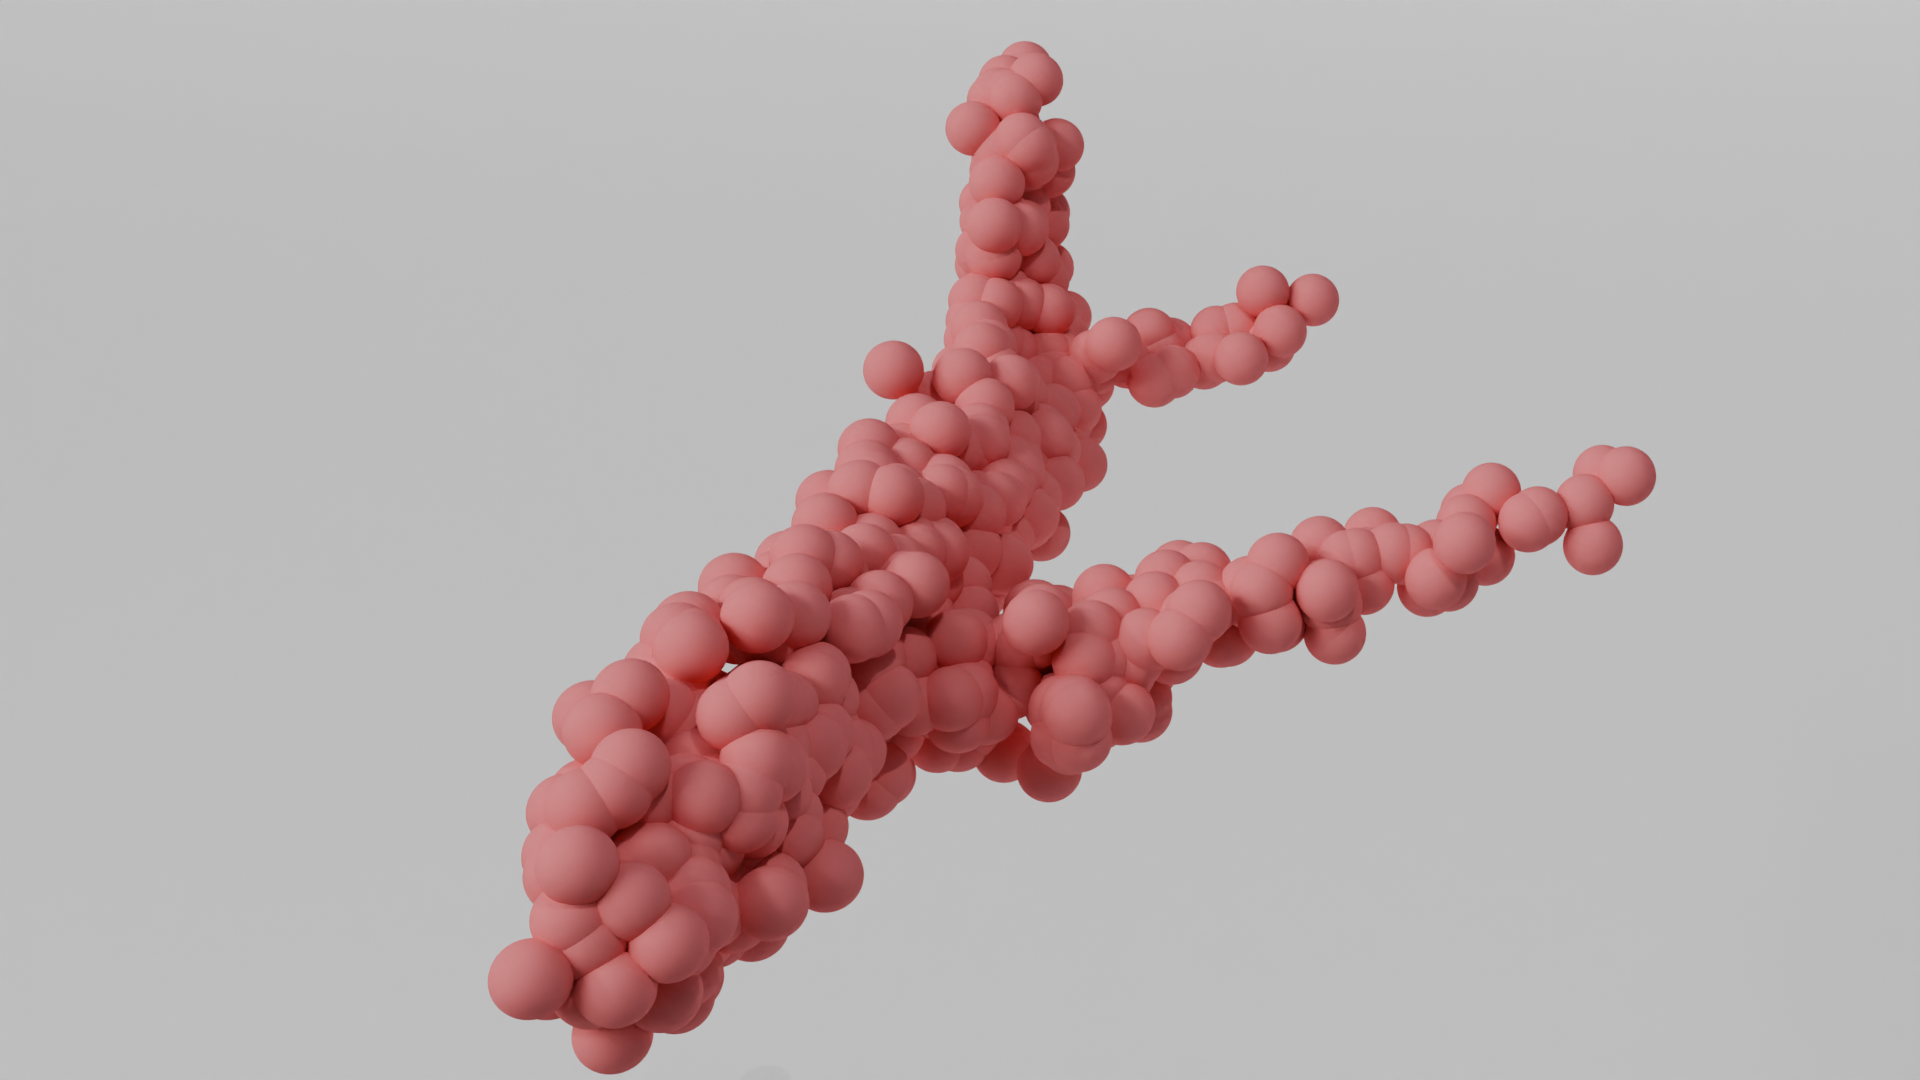
\includegraphics[width=\dimexpr\linewidth-20pt\relax]{figures/part_ap1.png}
            \makebox[20pt]{\raisebox{30pt}{\rotatebox[origin=c]{90}{\small DropCon}}}%
            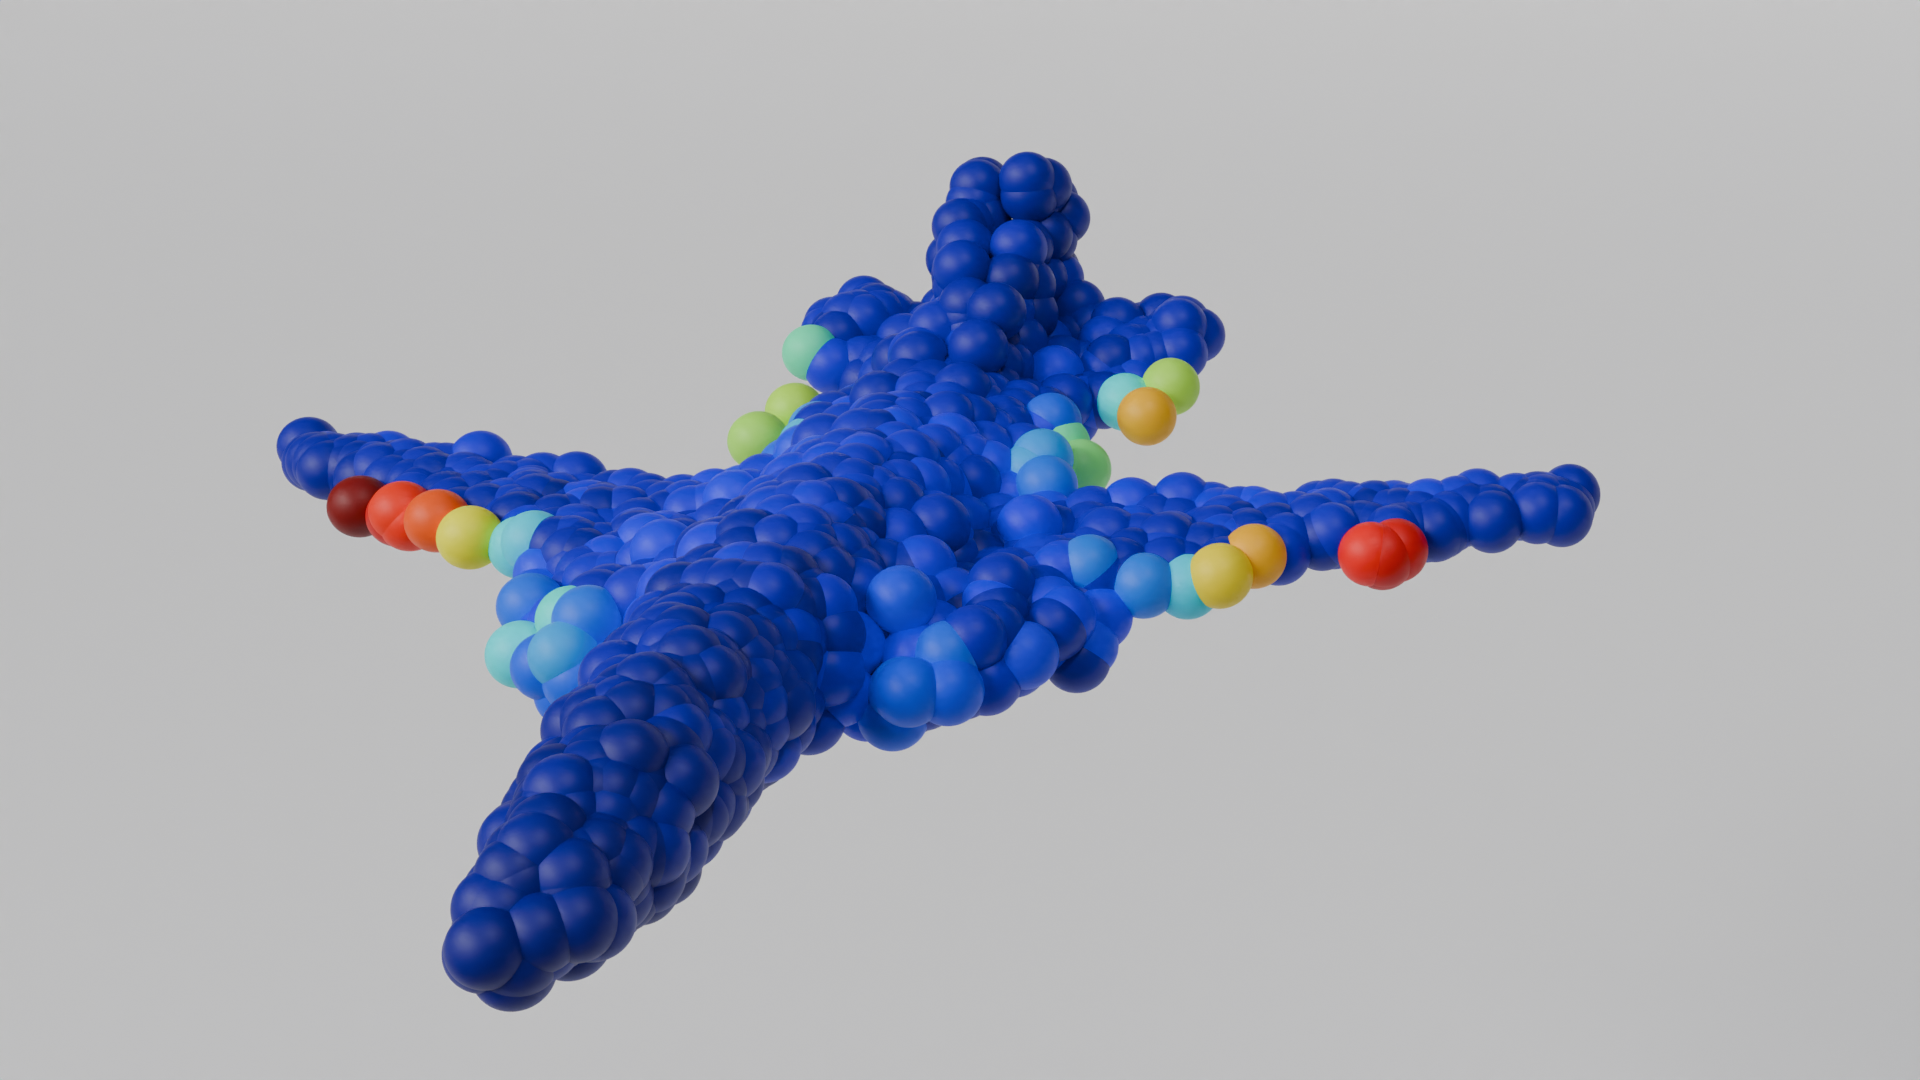
\includegraphics[width=\dimexpr\linewidth-20pt\relax]{figures/dc_lin_ap1.png}
            \makebox[20pt]{\raisebox{30pt}{\rotatebox[origin=c]{90}{\small Dropout}}}%
            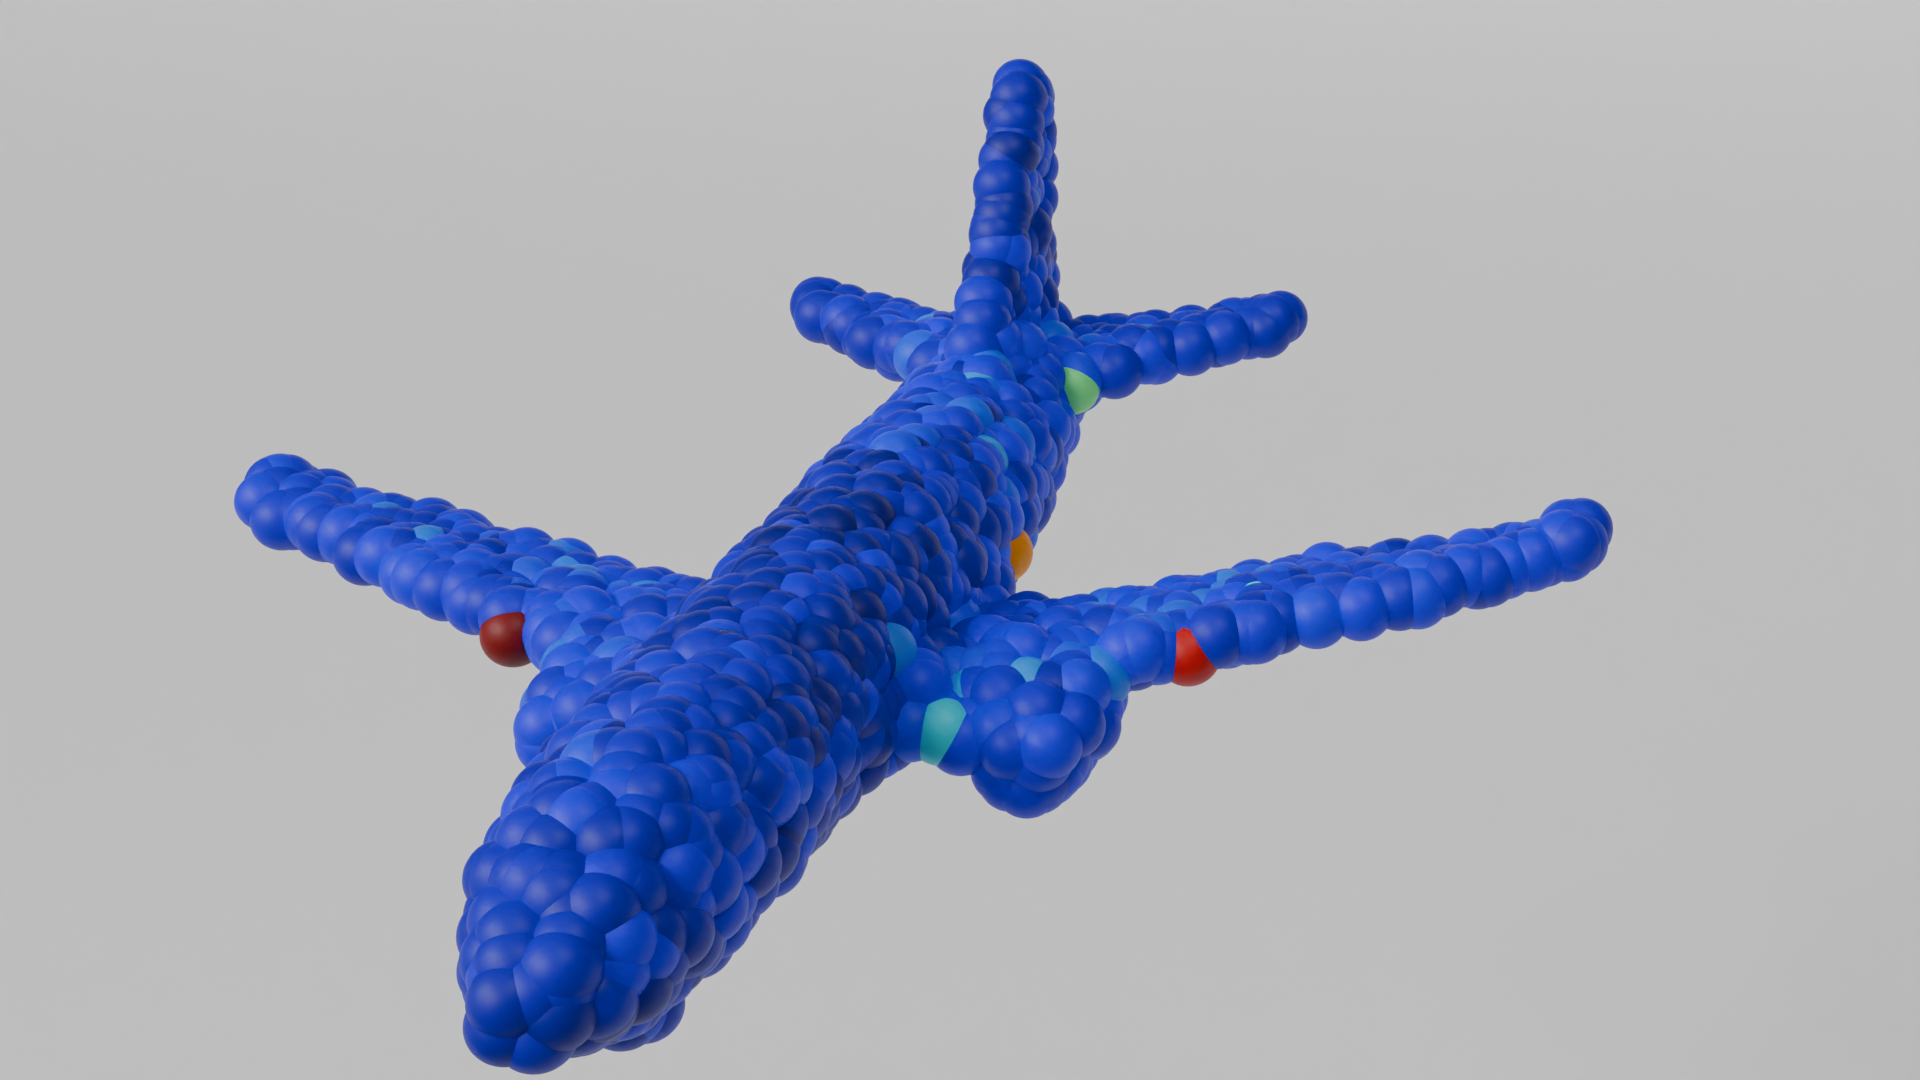
\includegraphics[width=\dimexpr\linewidth-20pt\relax]{figures/do_lin_ap1.png}
            \makebox[20pt]{\raisebox{30pt}{\rotatebox[origin=c]{90}{\small Ensemble}}}%
            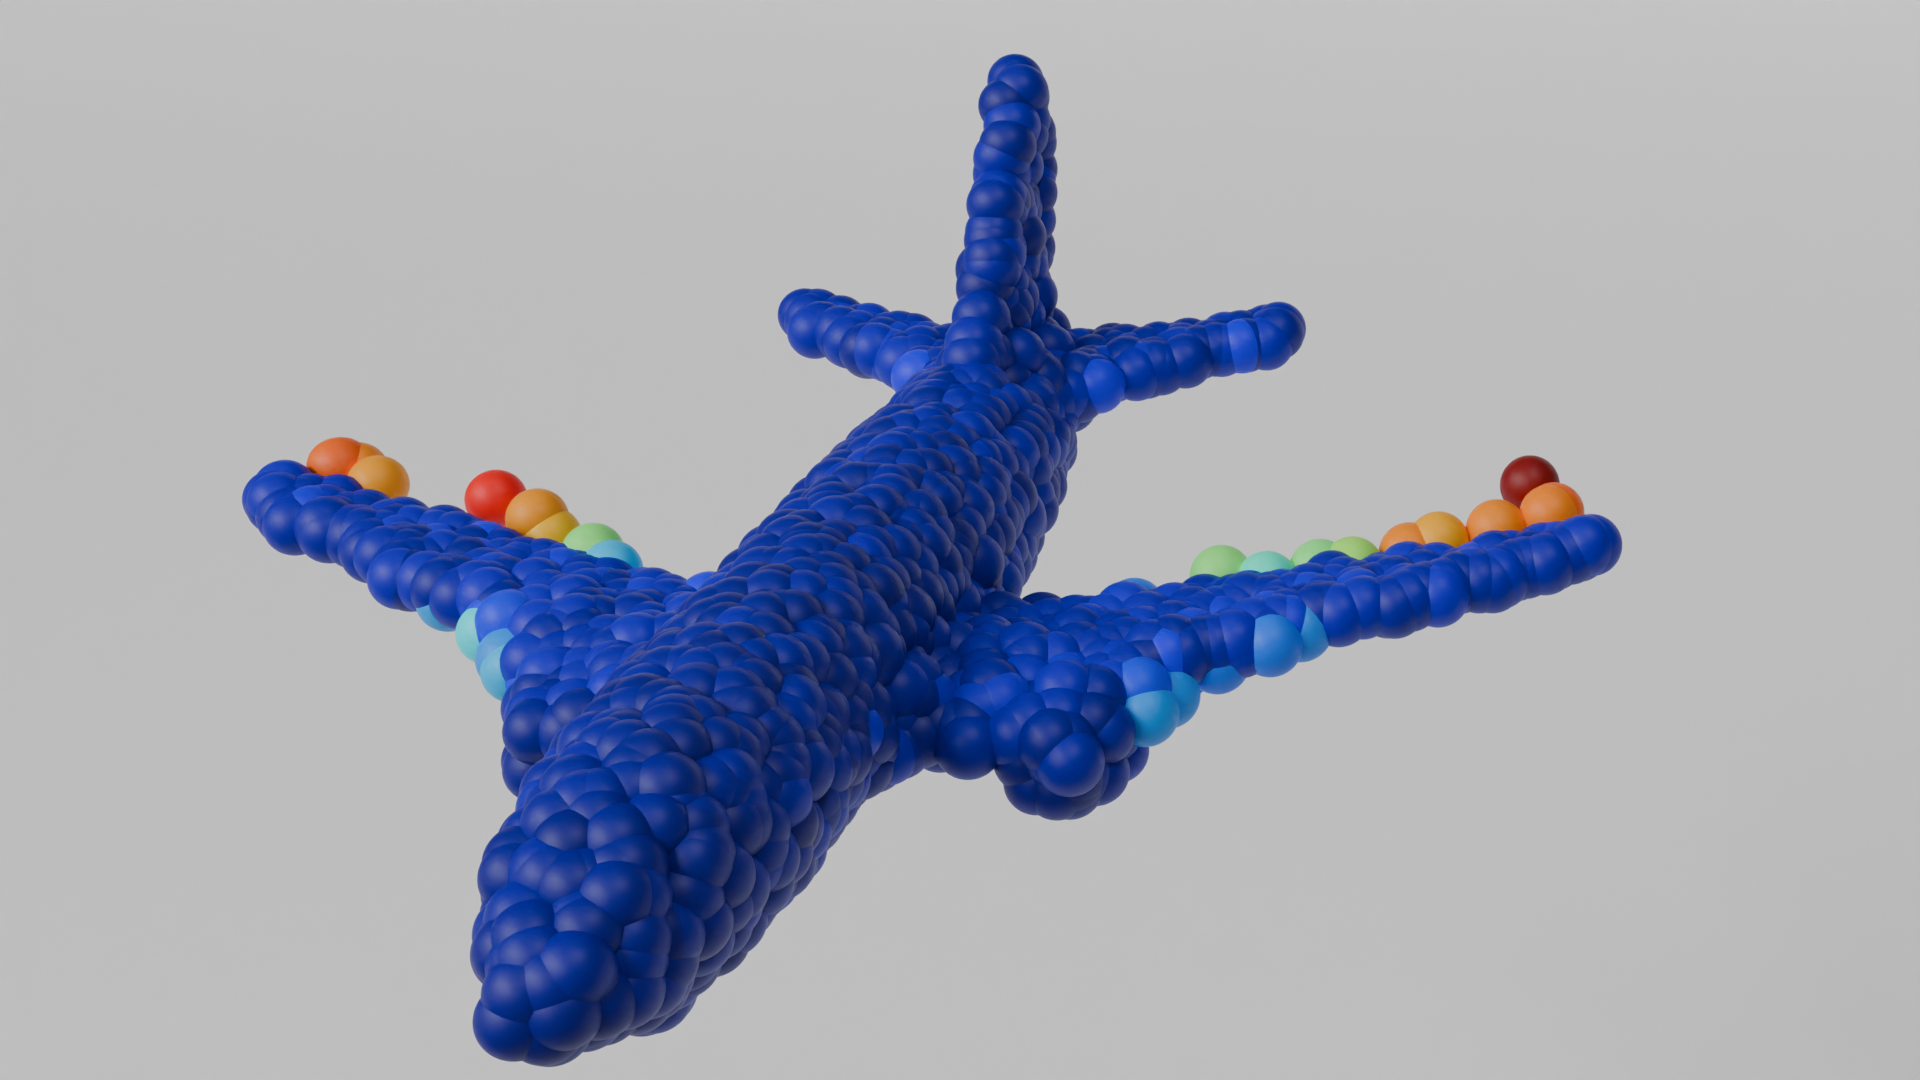
\includegraphics[width=\dimexpr\linewidth-20pt\relax]{figures/ens_lin_ap1.png}
            \makebox[20pt]{\raisebox{30pt}{\rotatebox[origin=c]{90}{\small Implicit}}}%
            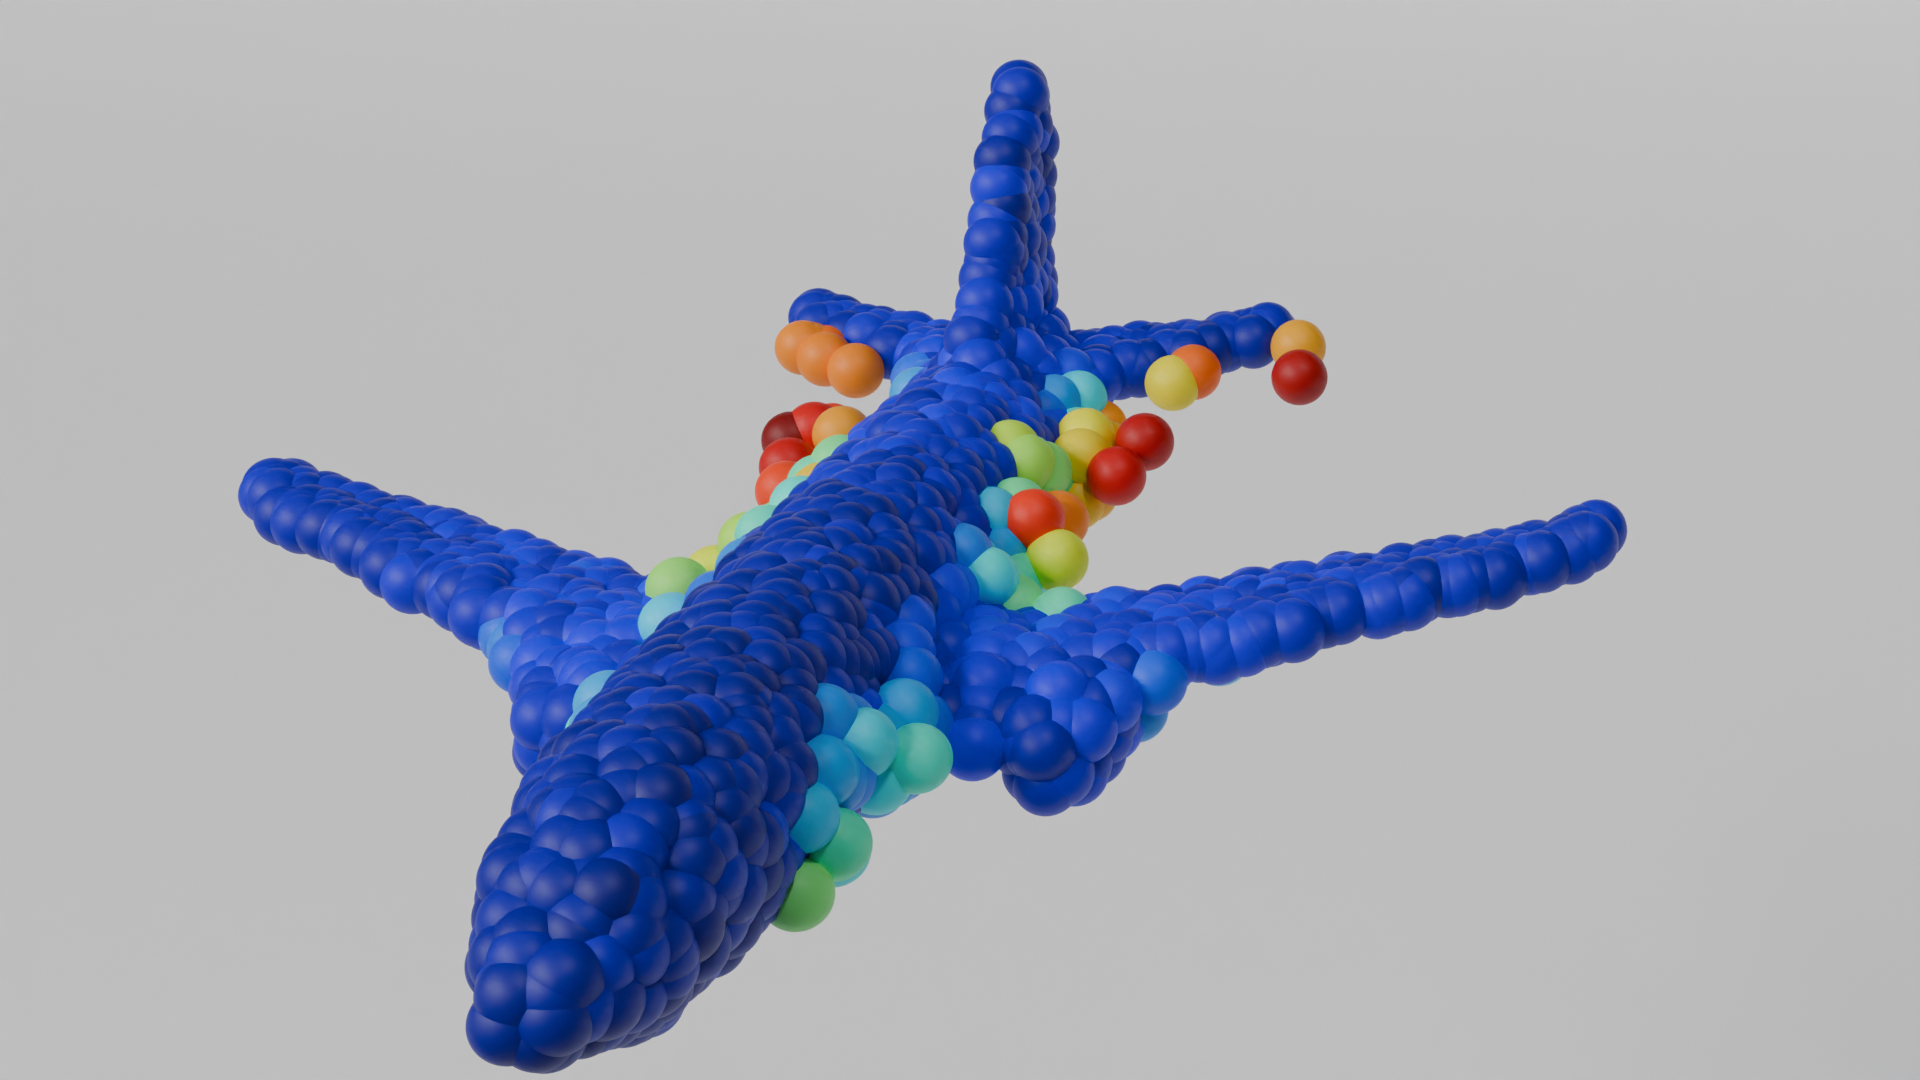
\includegraphics[width=\dimexpr\linewidth-20pt\relax]{figures/iml_lin_ap1.png}
            \makebox[20pt]{\raisebox{30pt}{\rotatebox[origin=c]{90}{\small GT}}}%
            \includegraphics[width=\dimexpr\linewidth-20pt\relax]{figures/com_ap1.png}
            \caption{Airplane 1}
          \end{subfigure}\hfill
          \begin{subfigure}[t]{0.315\textwidth}
            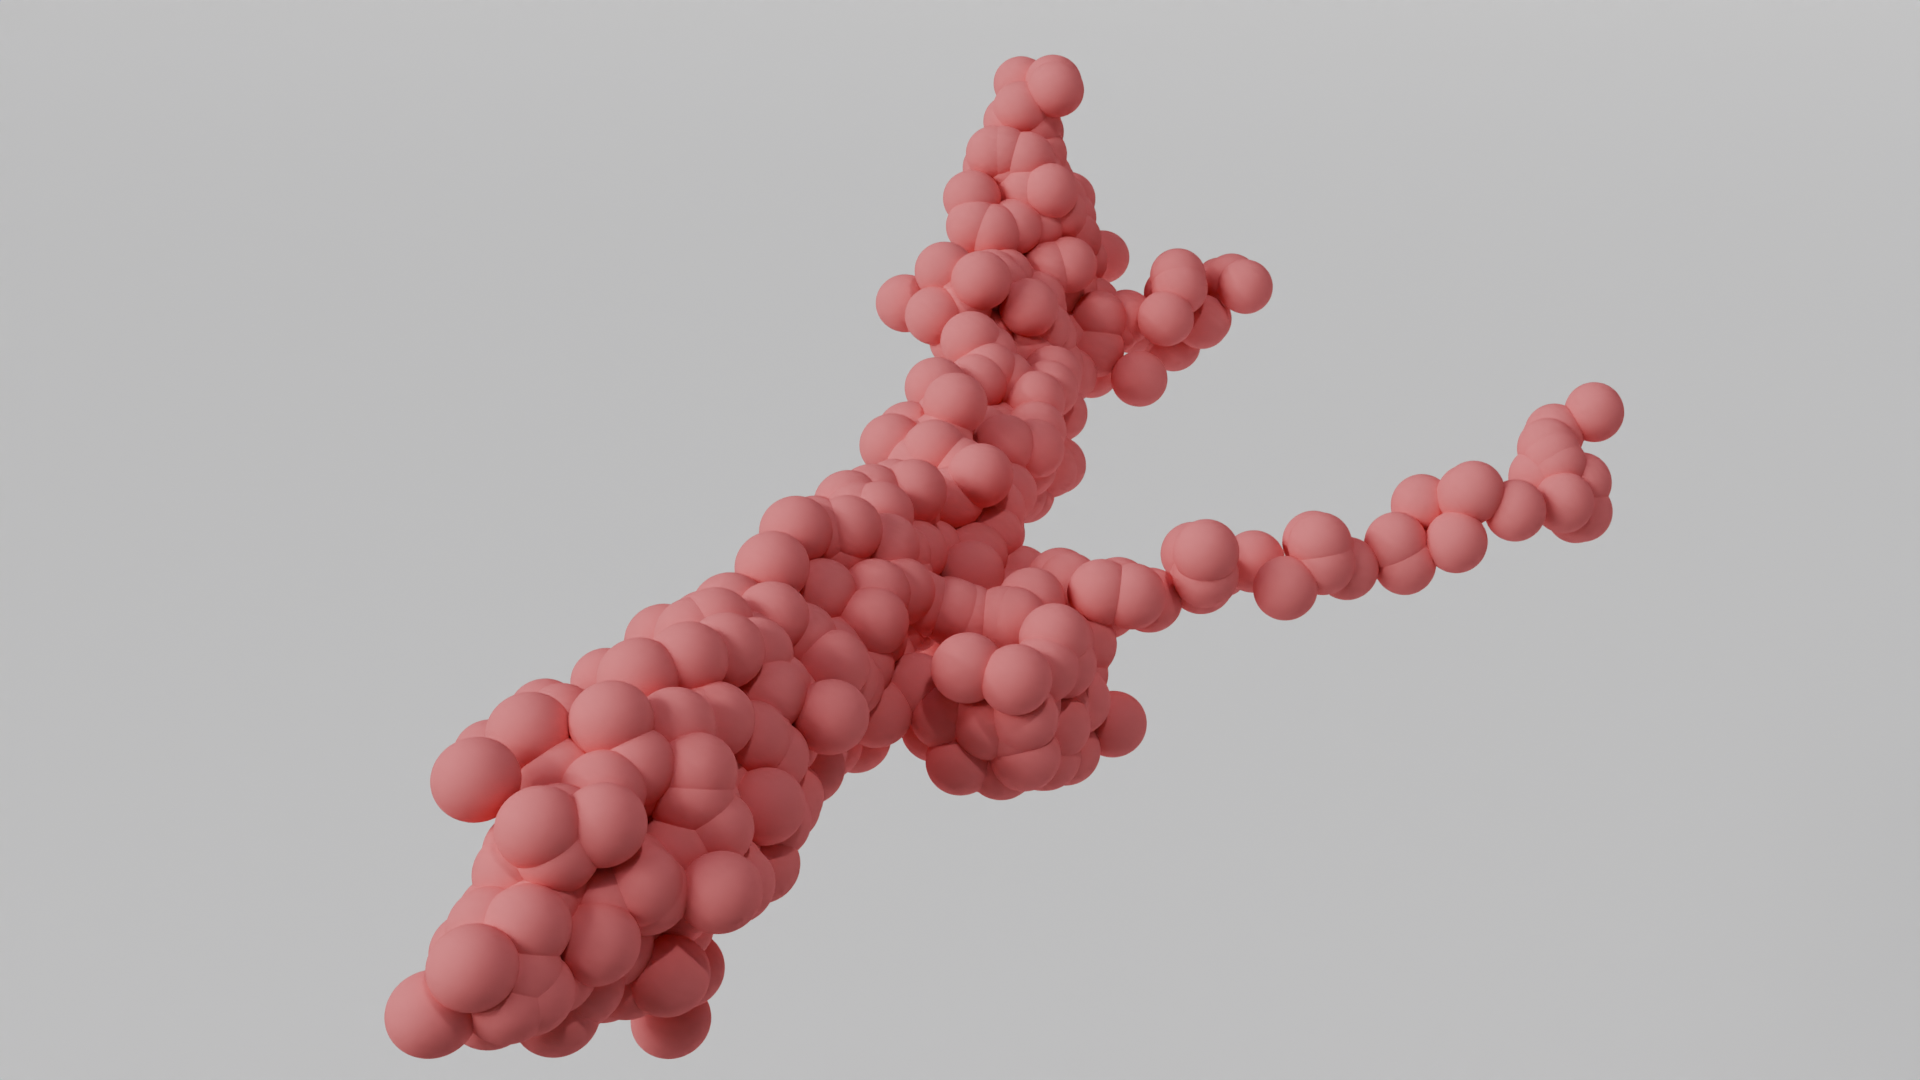
\includegraphics[width=\textwidth]{figures/part_ap2.png}
            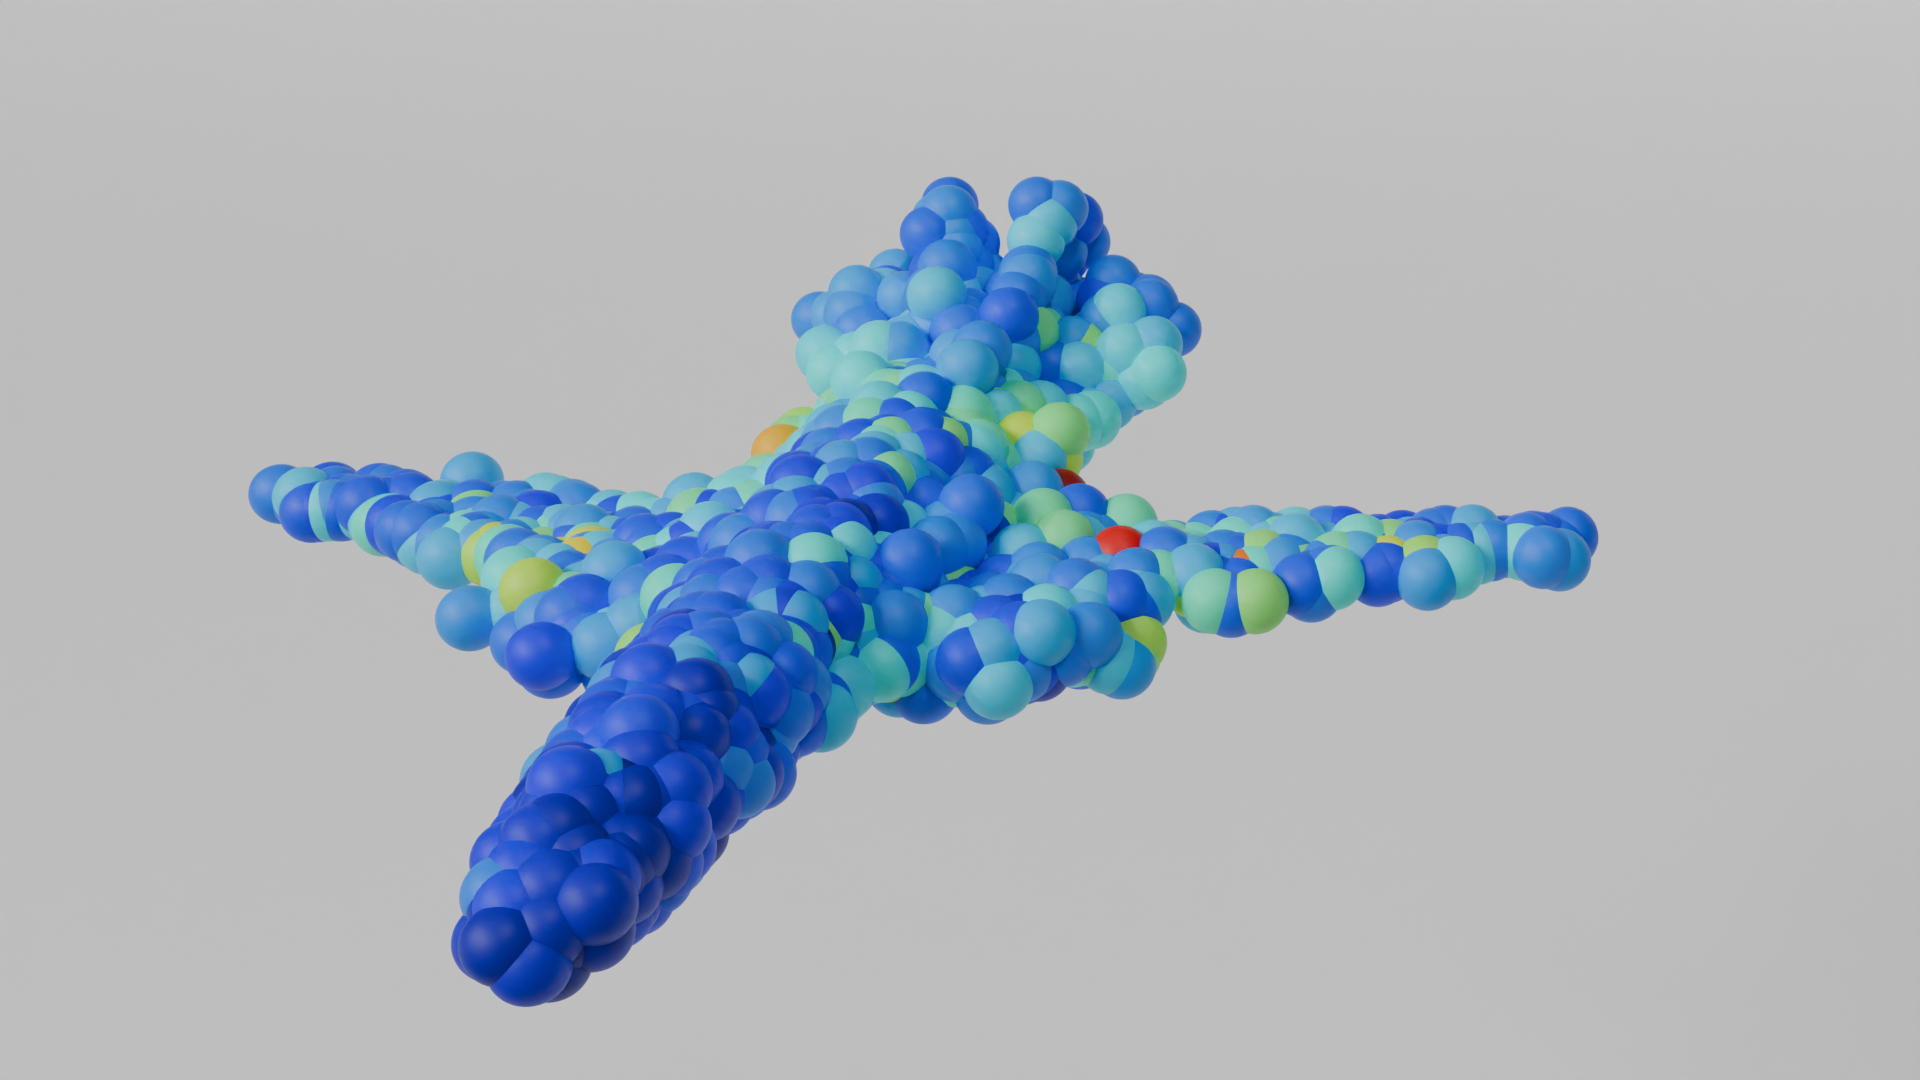
\includegraphics[width=\textwidth]{figures/dc_lin_ap2.png}
            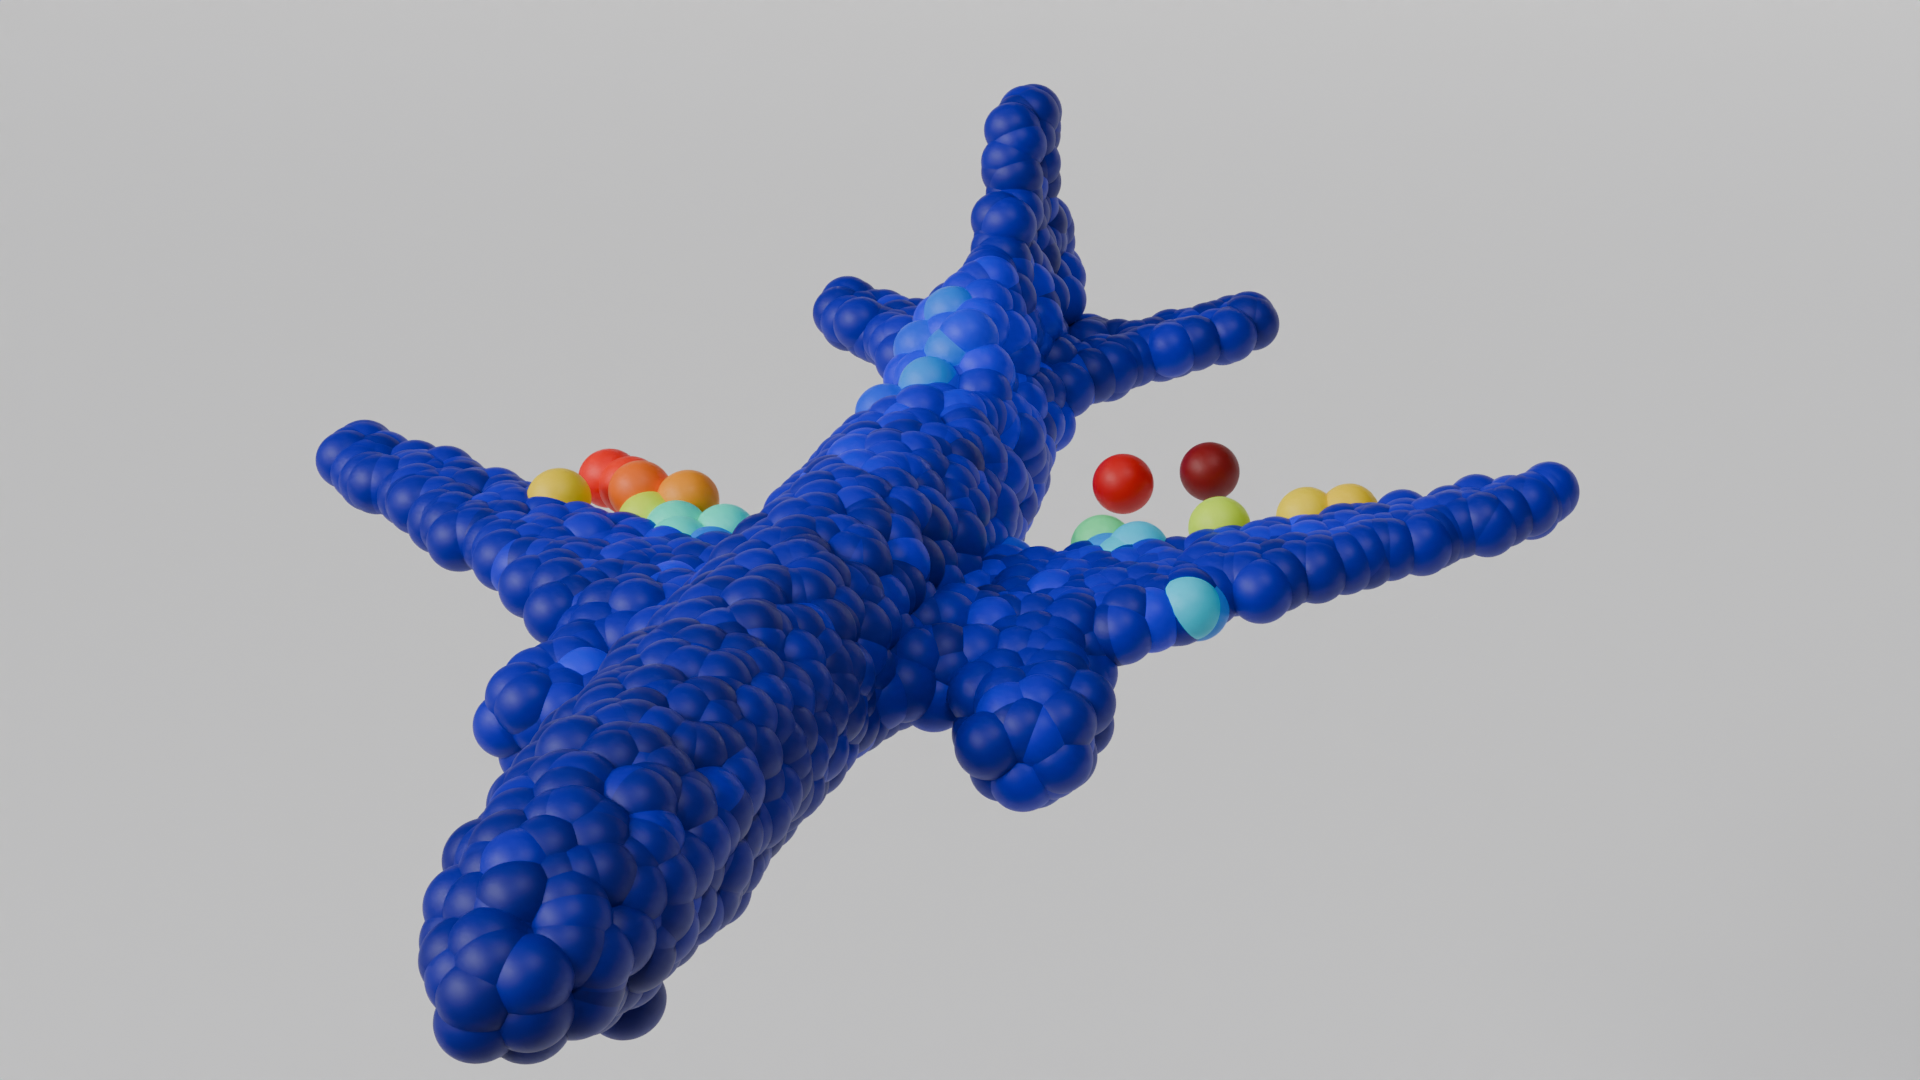
\includegraphics[width=\textwidth]{figures/do_lin_ap2.png}
            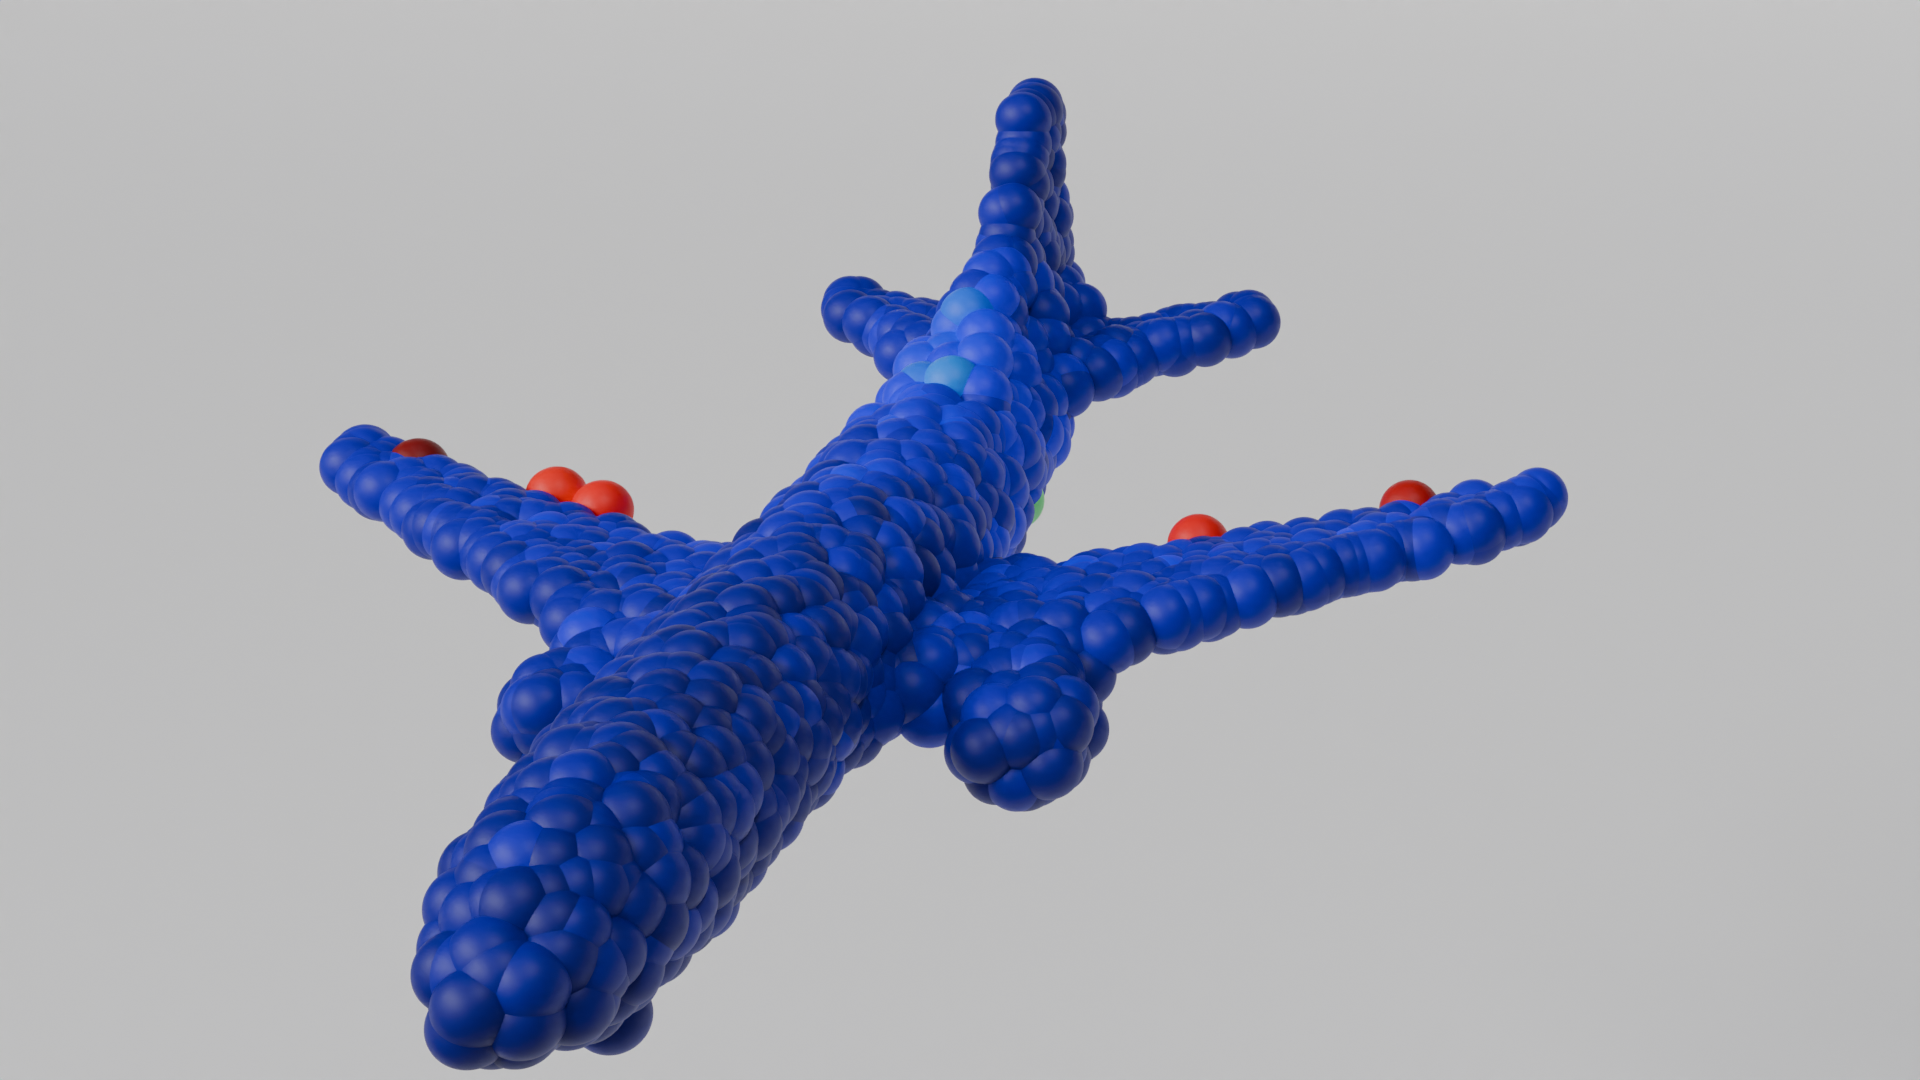
\includegraphics[width=\textwidth]{figures/ens_lin_ap2.png}
            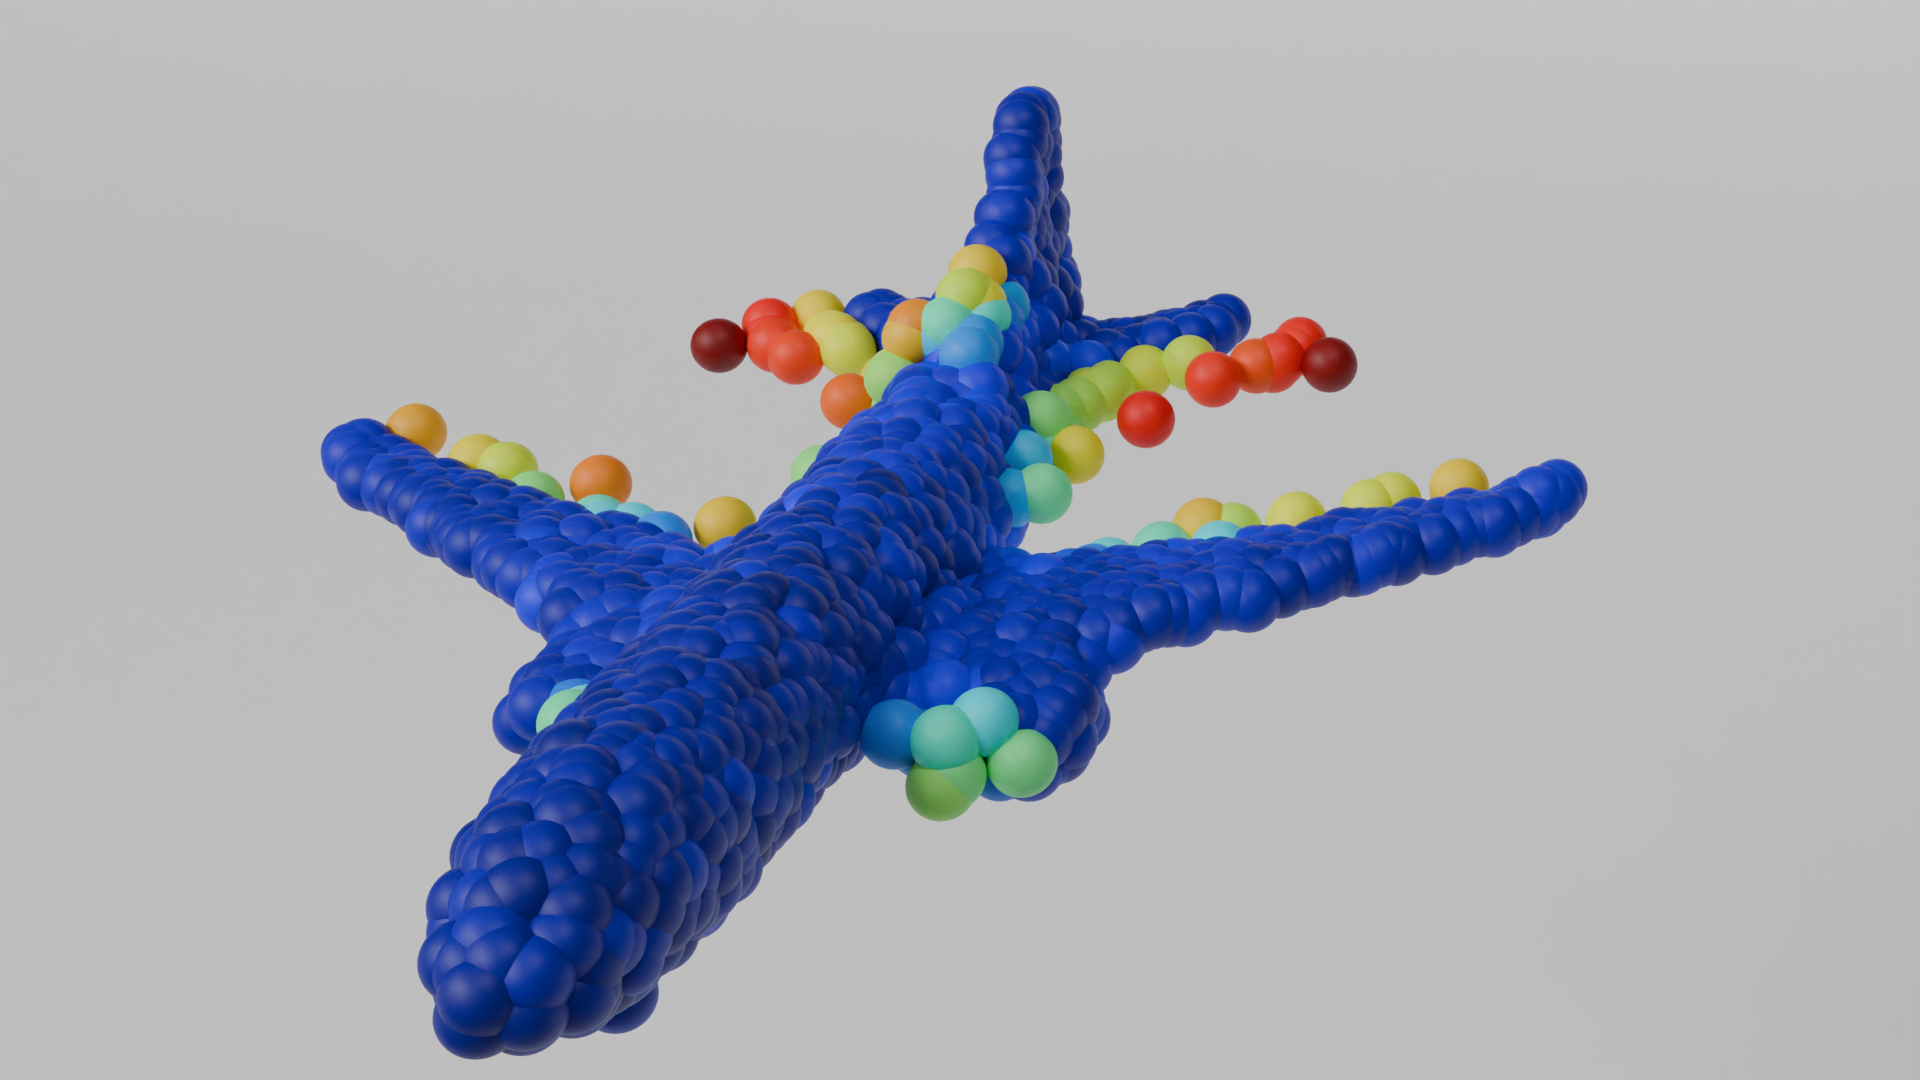
\includegraphics[width=\textwidth]{figures/iml_lin_ap2.png}
            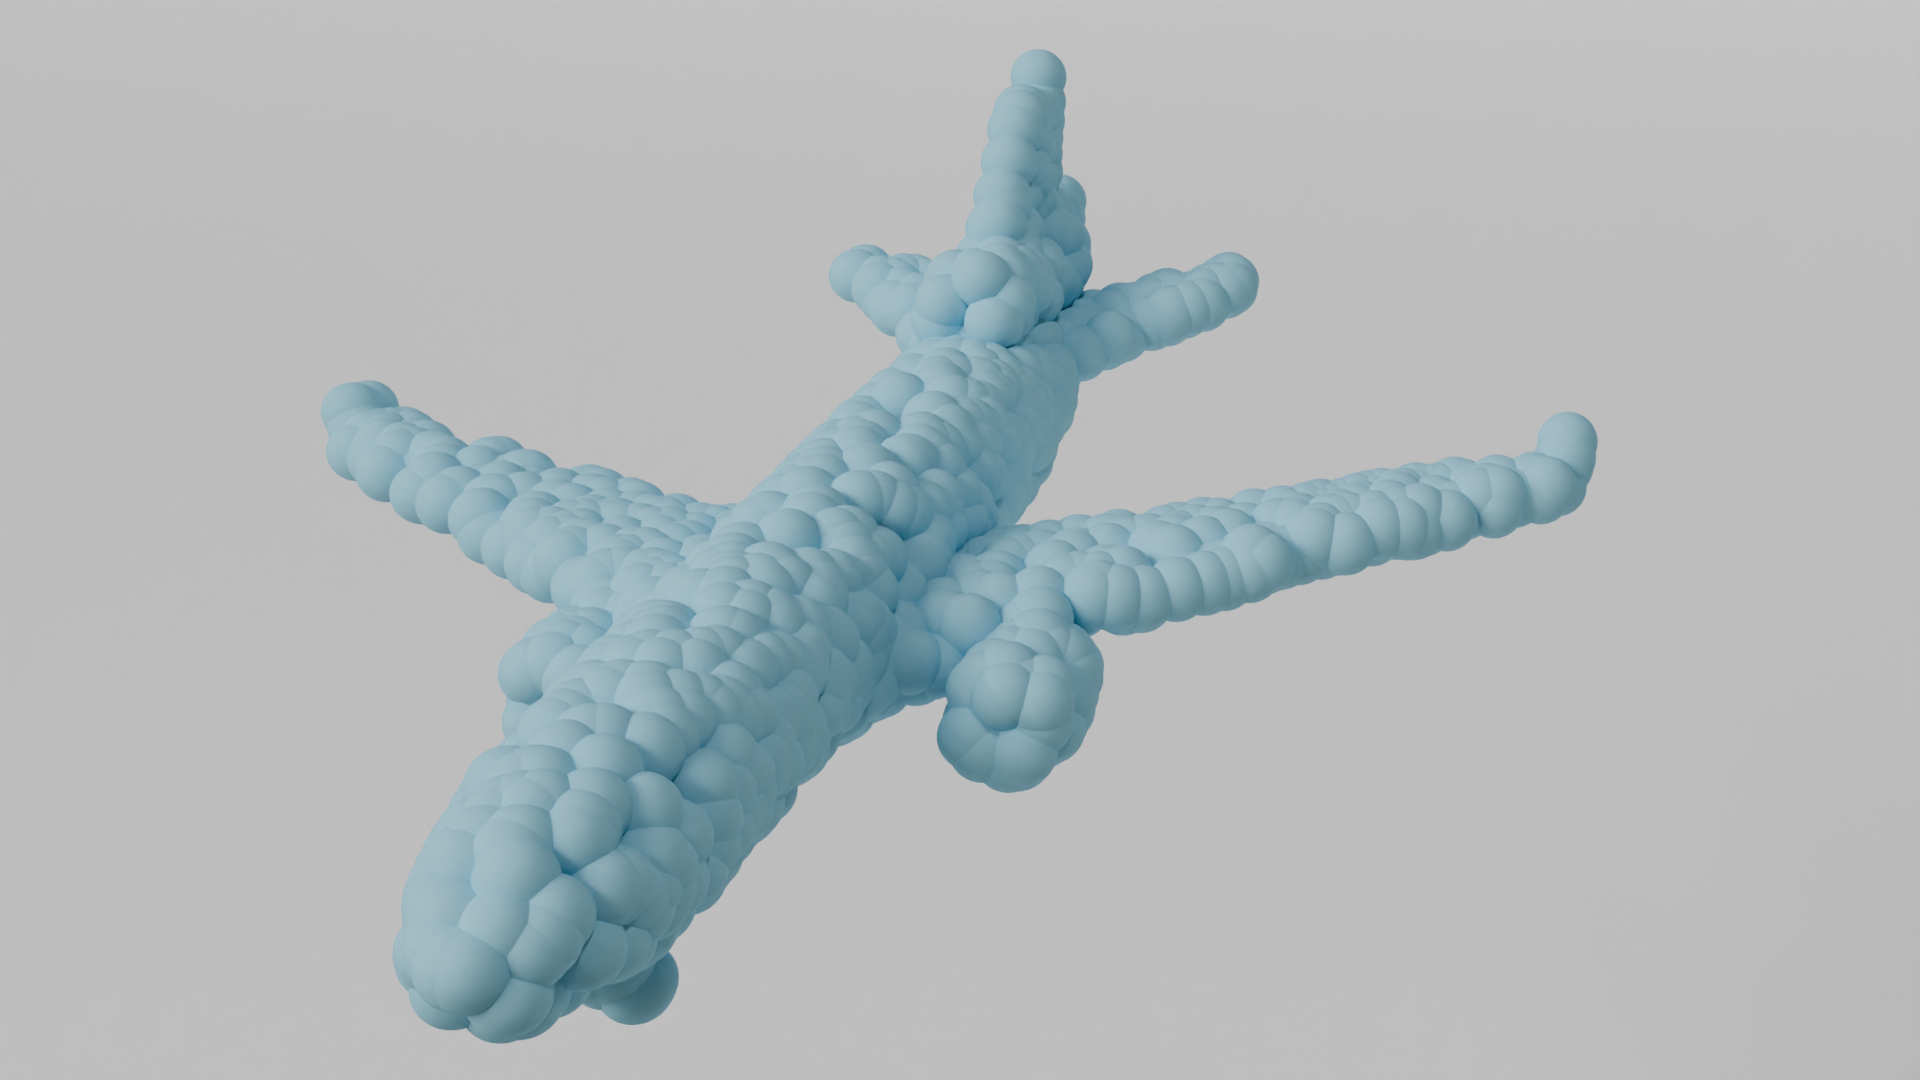
\includegraphics[width=\textwidth]{figures/com_ap2.png}
            \caption{Airplane 2}
          \end{subfigure}\hfill
          \begin{subfigure}[t]{0.315\textwidth}
            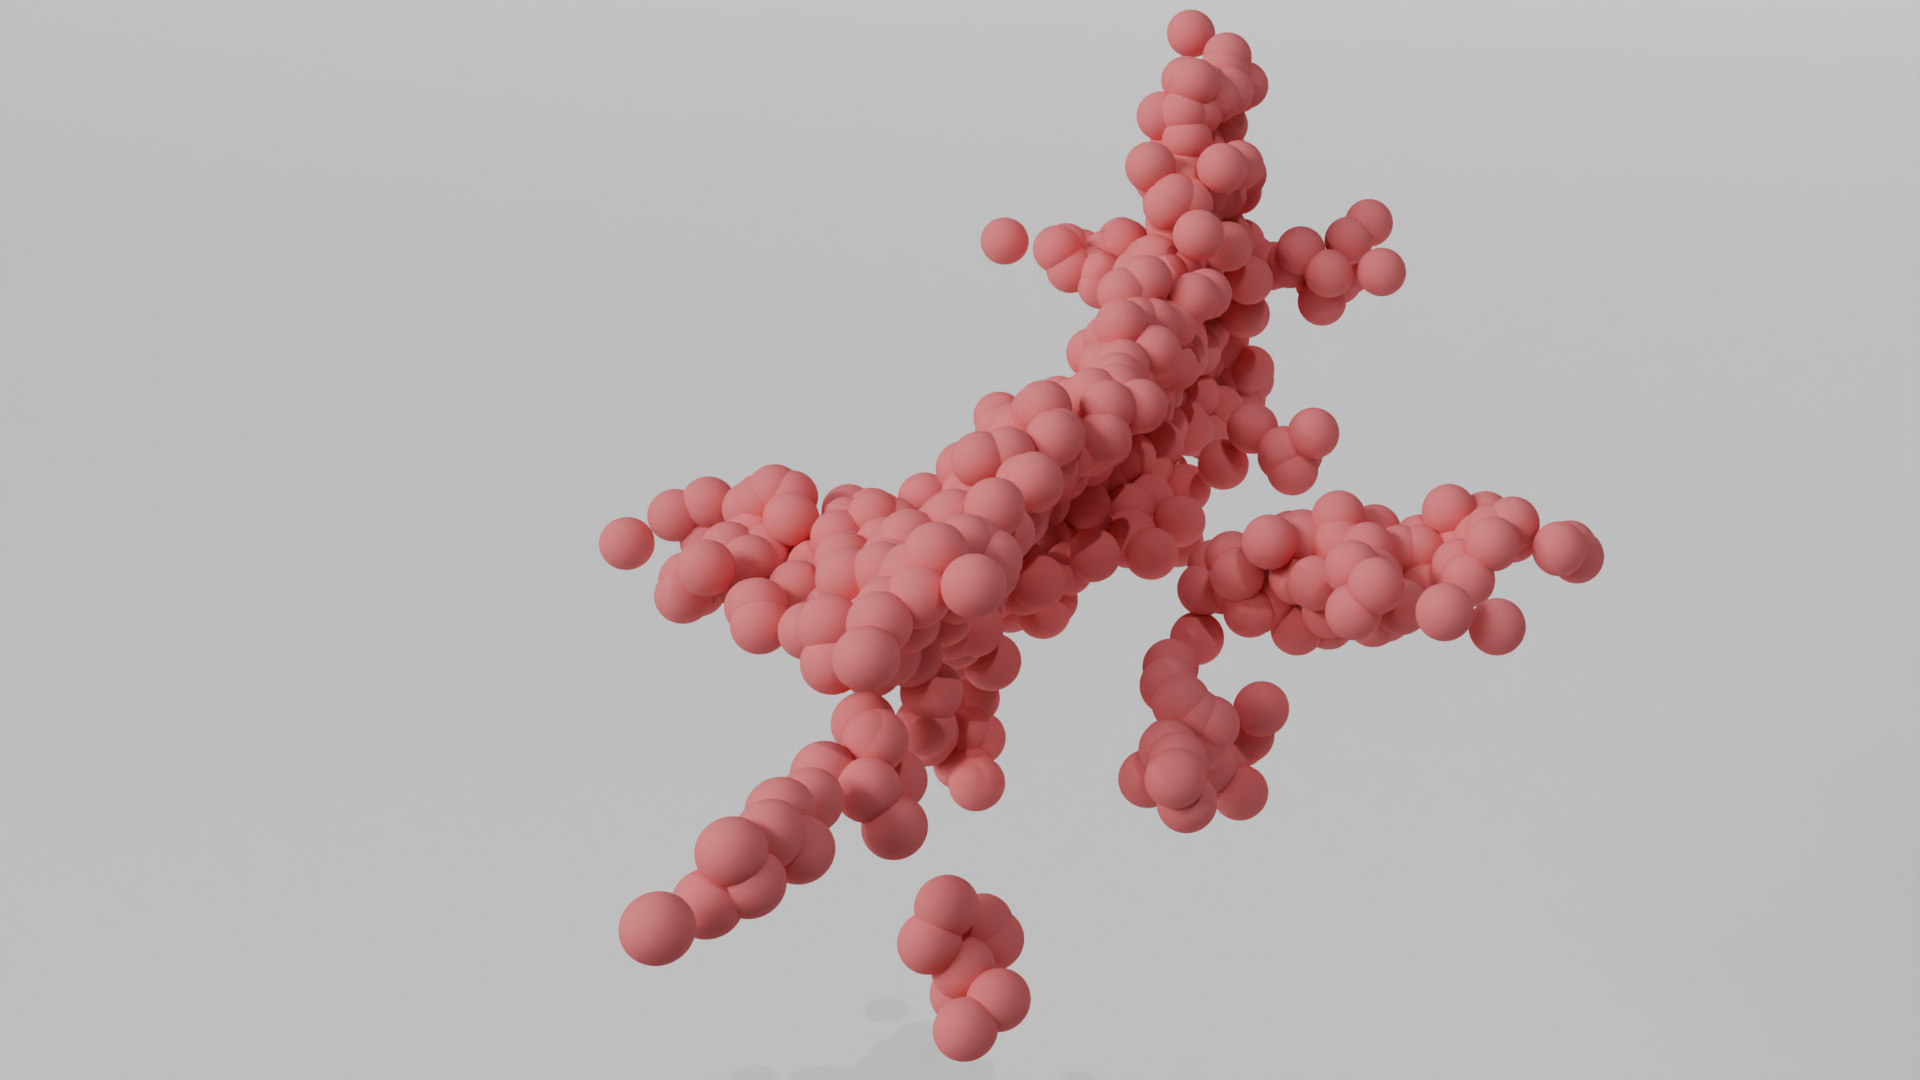
\includegraphics[width=\textwidth]{figures/part_ap3.png}
            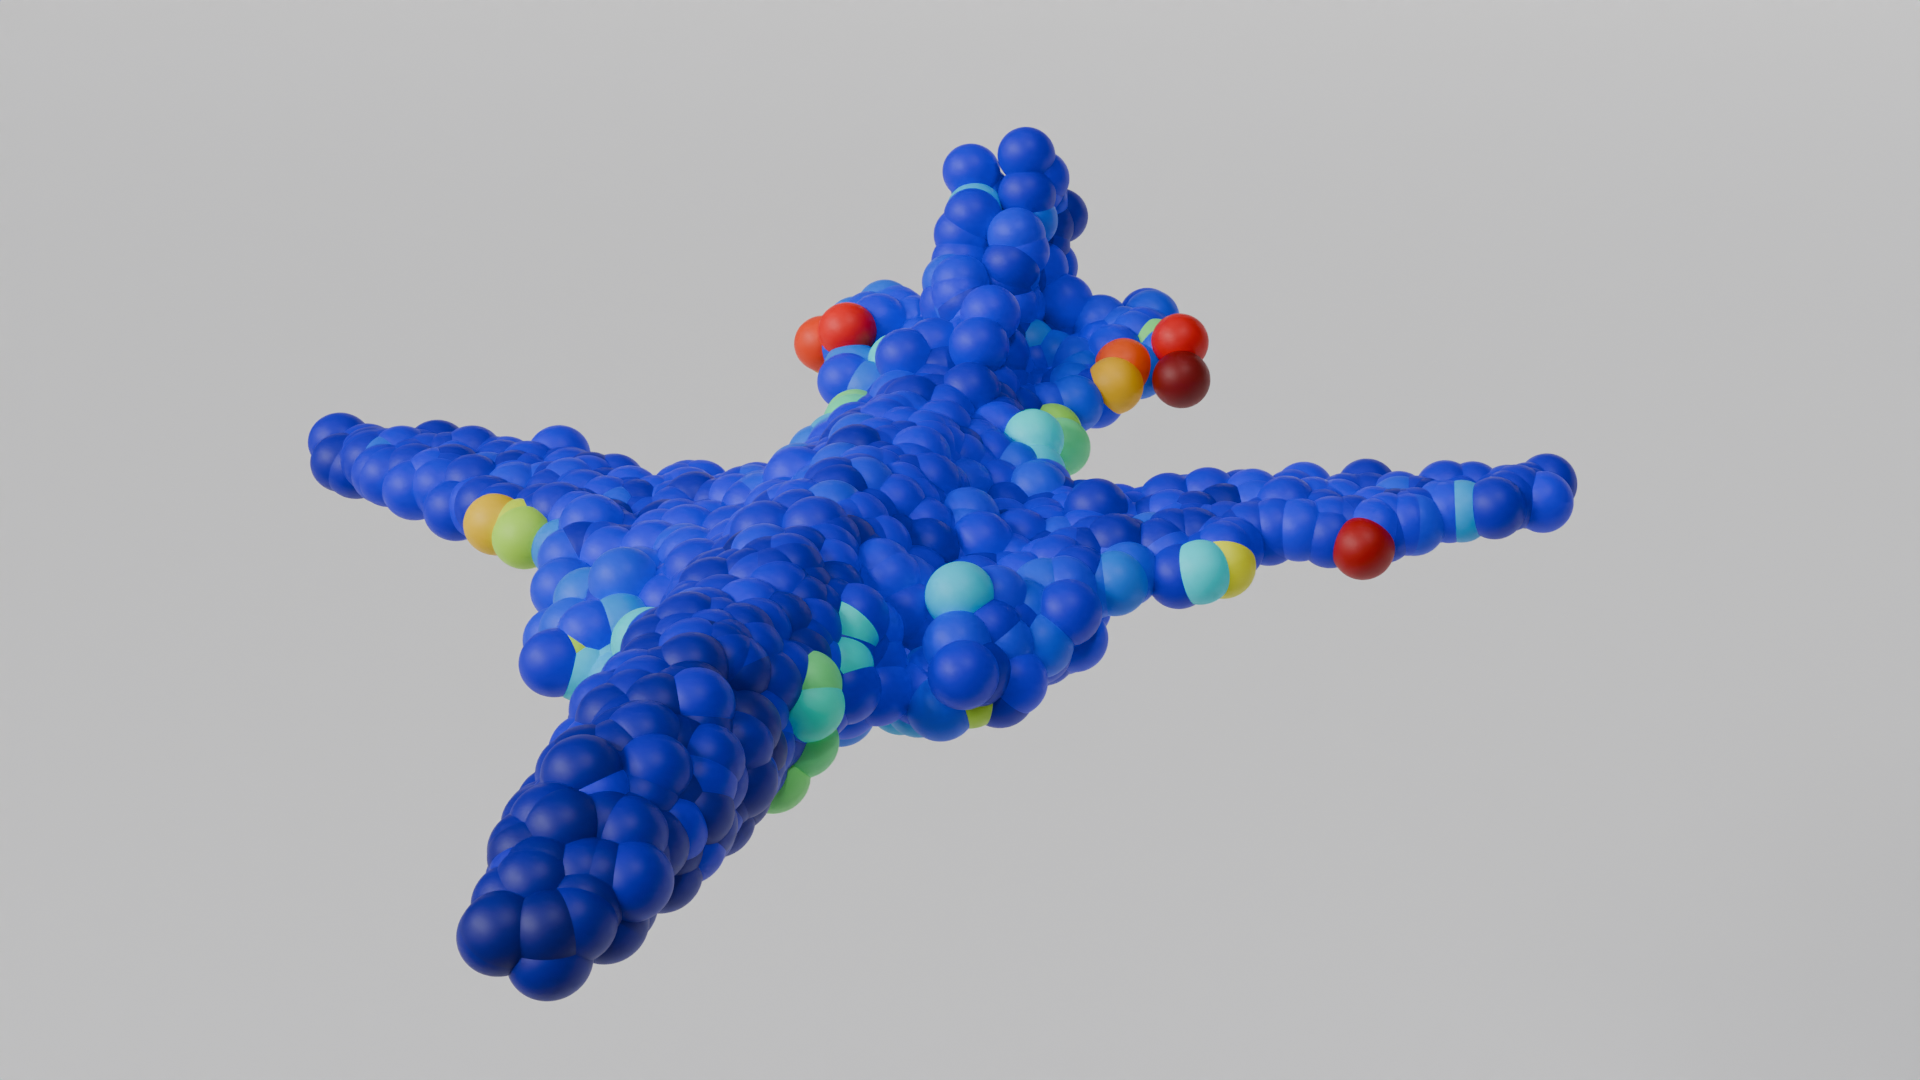
\includegraphics[width=\textwidth]{figures/dc_lin_ap3.png}
            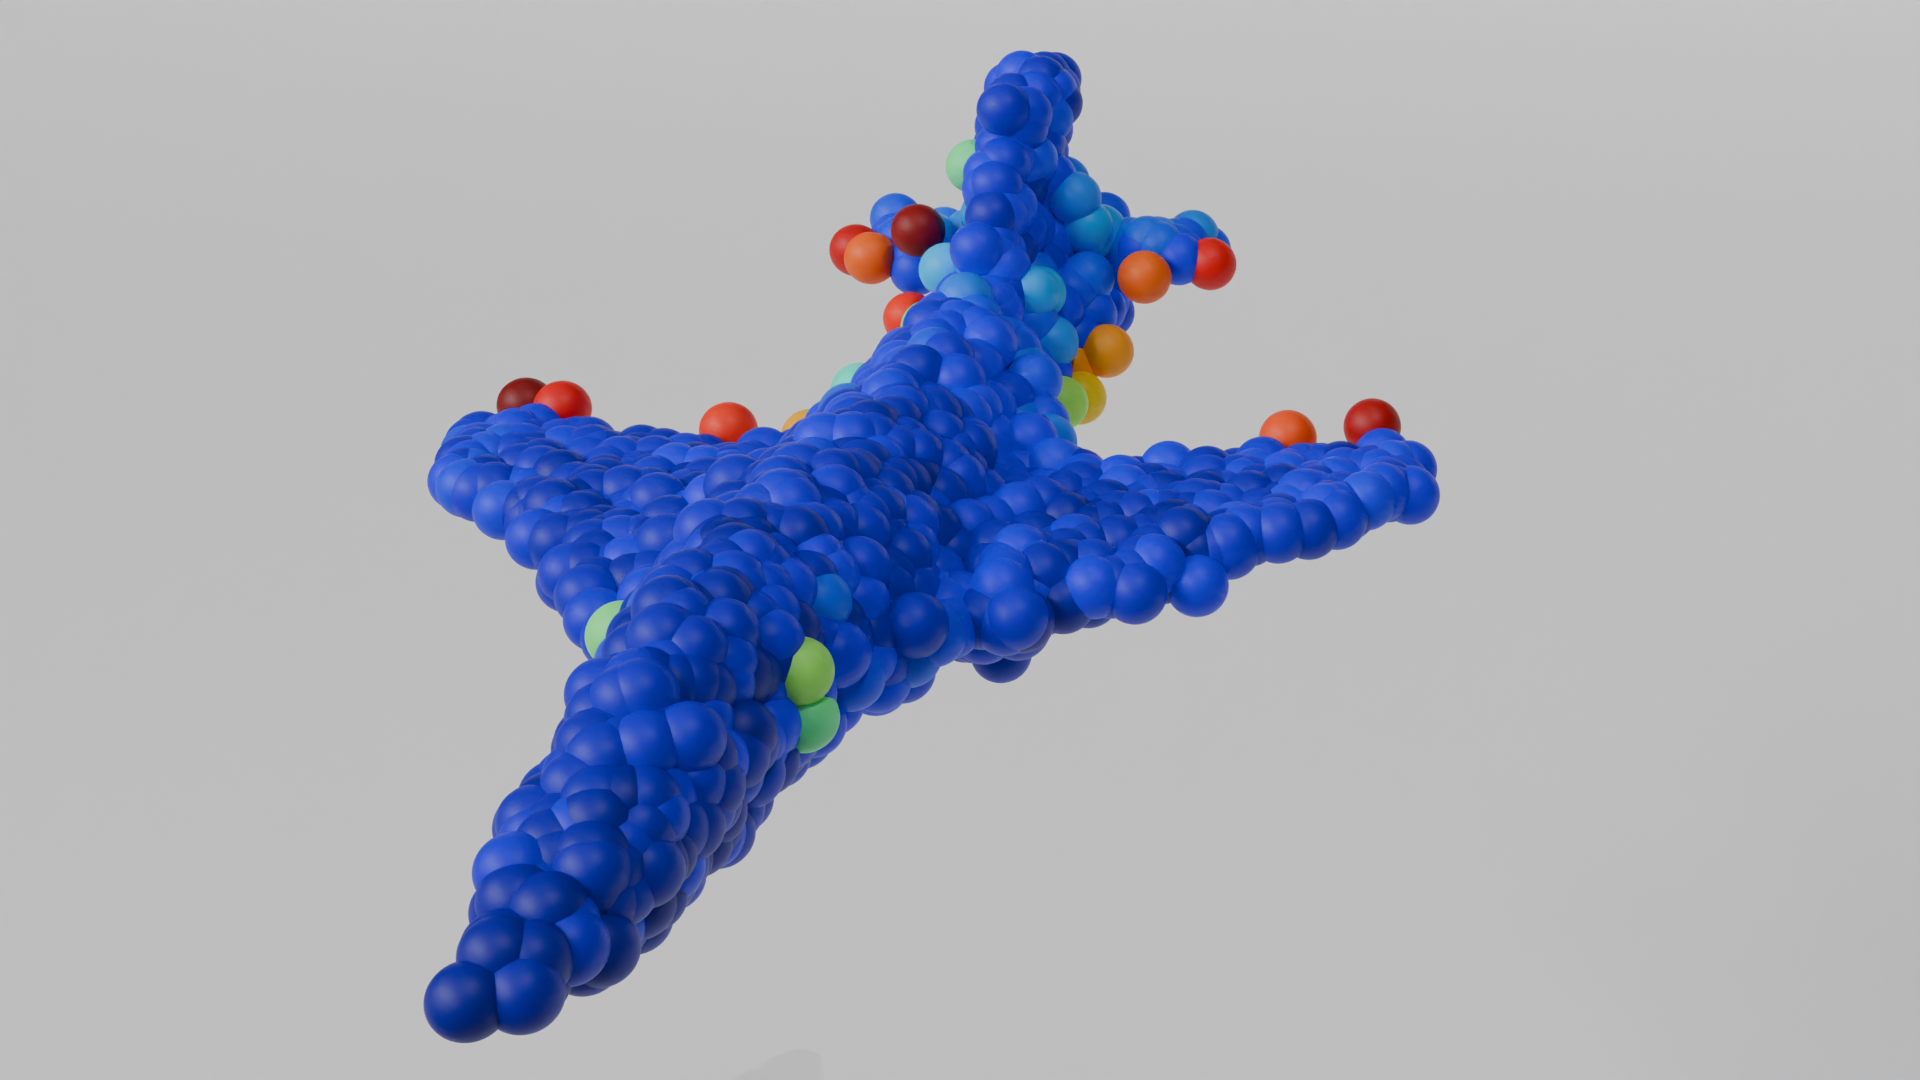
\includegraphics[width=\textwidth]{figures/do_lin_ap3.png}
            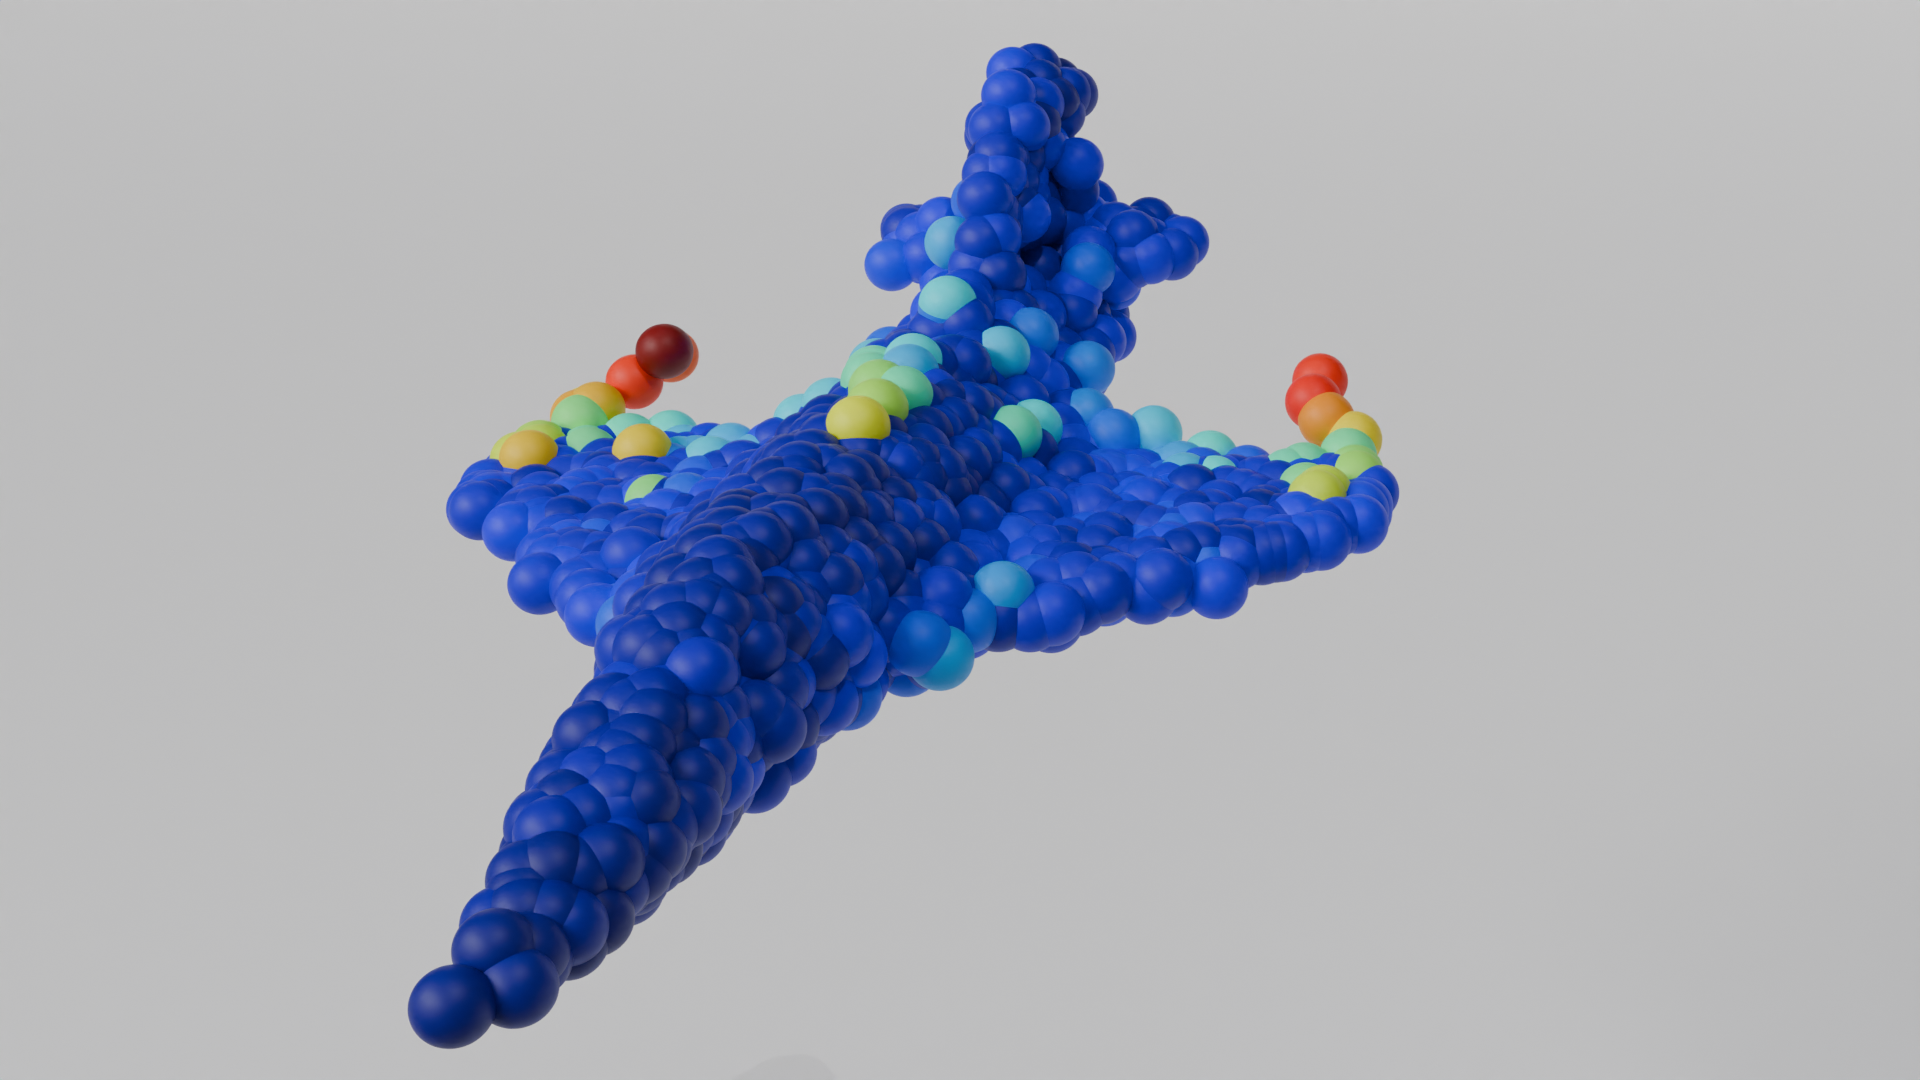
\includegraphics[width=\textwidth]{figures/ens_lin_ap3.png}
            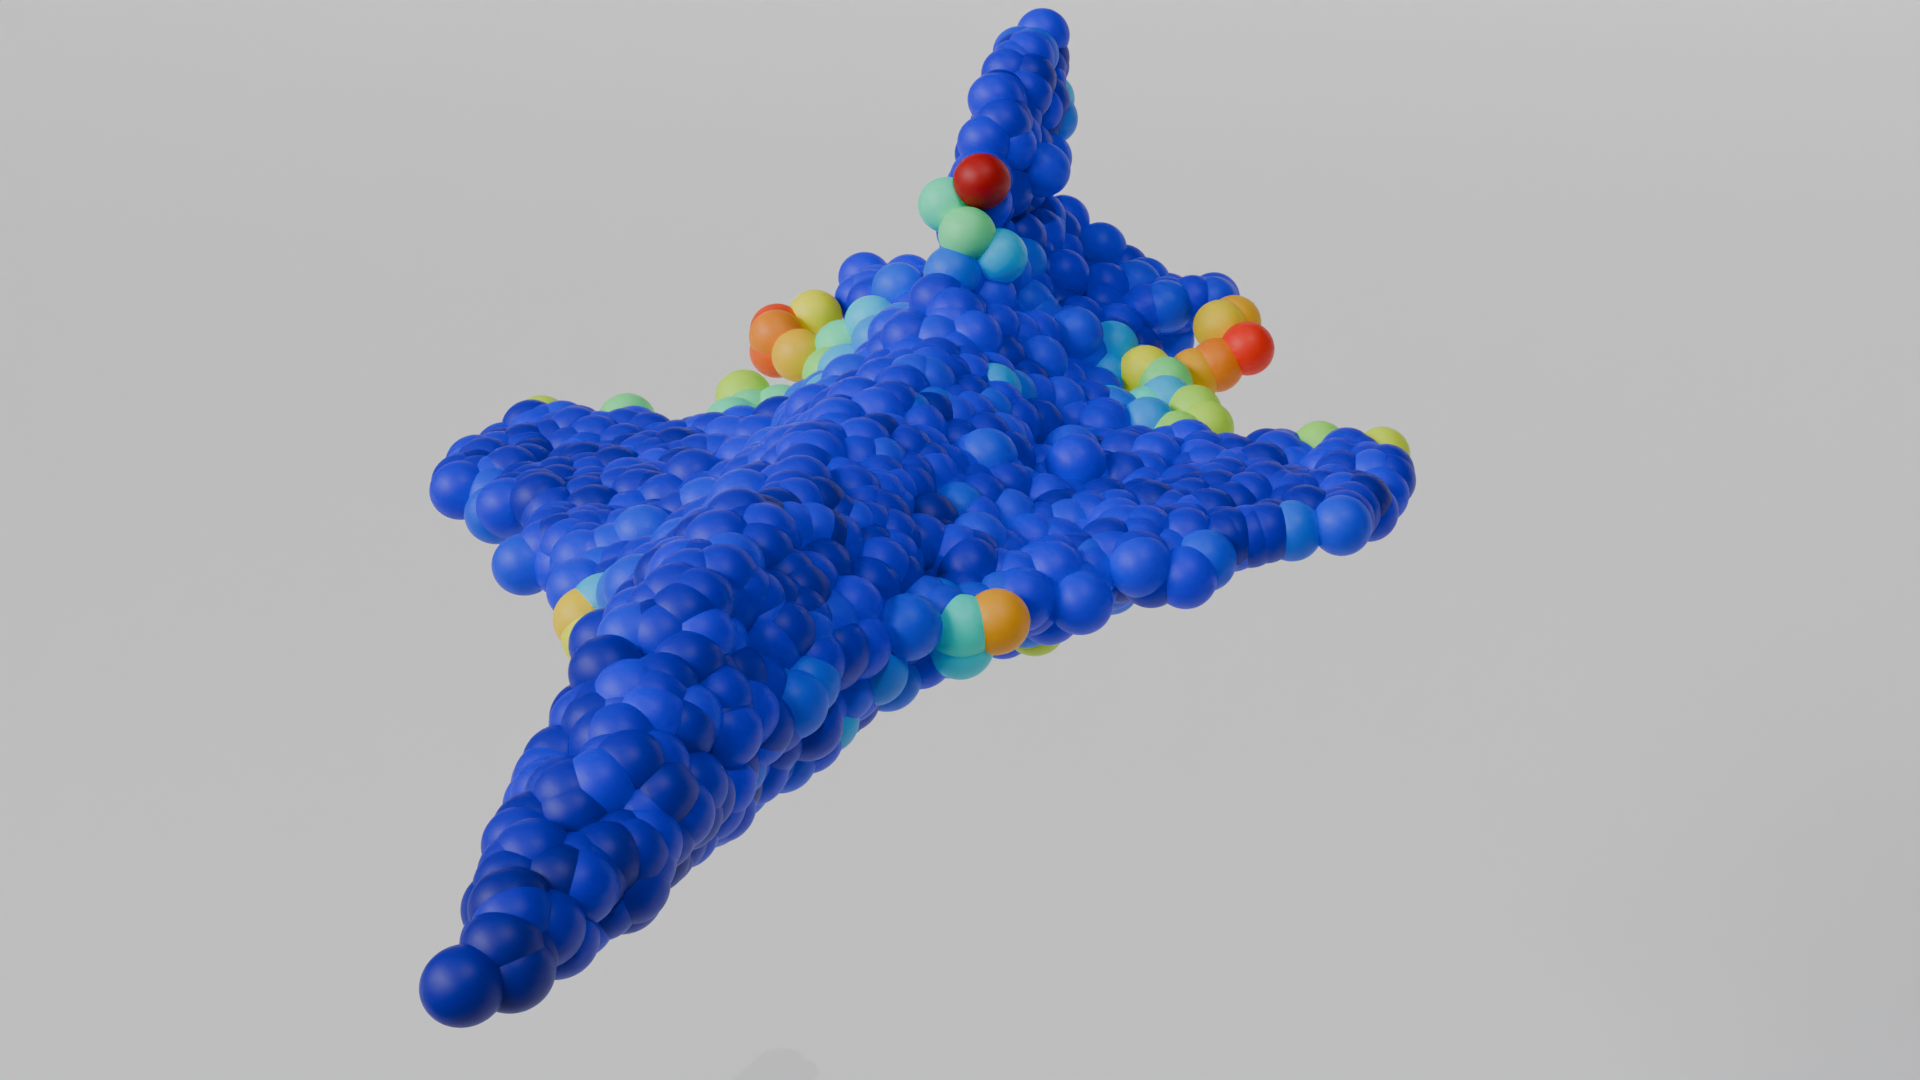
\includegraphics[width=\textwidth]{figures/iml_lin_ap3.png}
            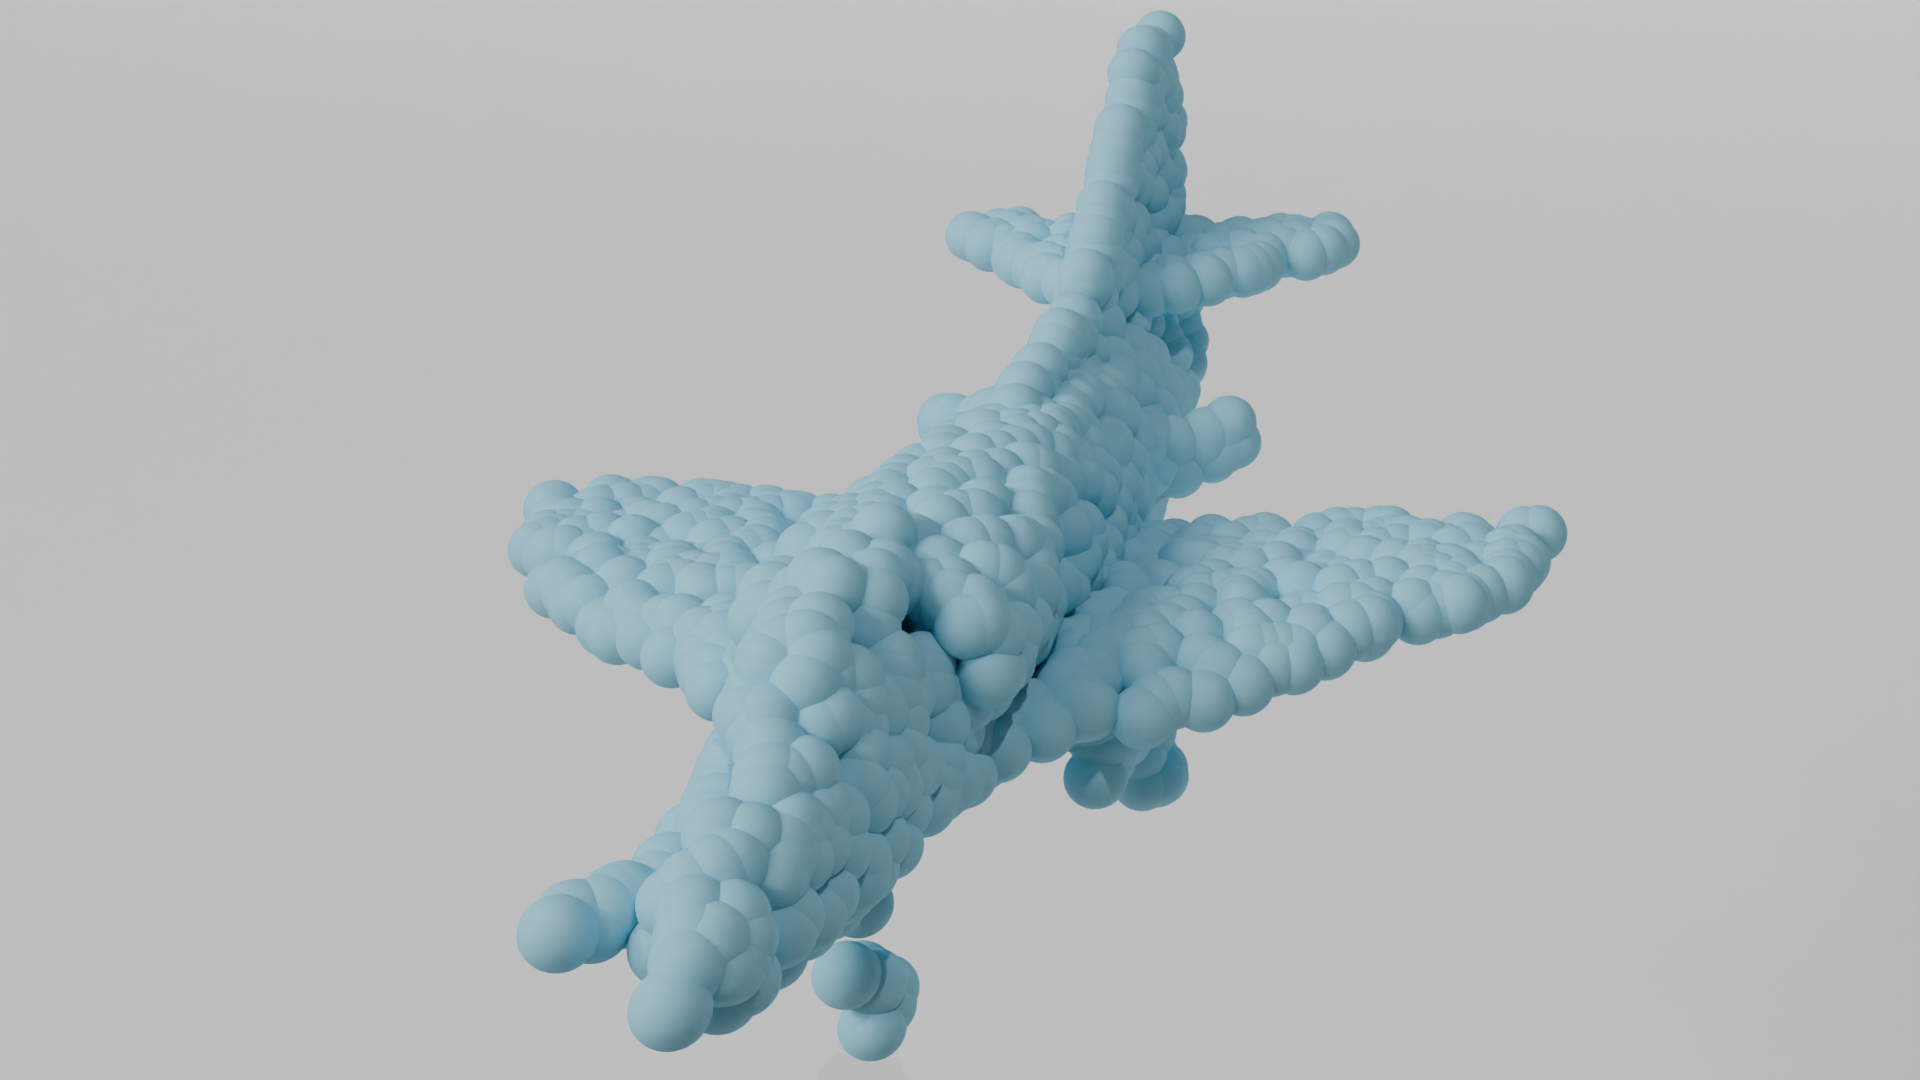
\includegraphics[width=\textwidth]{figures/com_ap3.png}
            \caption{Airplane 3}
          \end{subfigure}
          \caption{Qualitative comparison between different empirical uncertainty quantification methods for point cloud completion on the airplane subcategory of ShapeNet data. Input refers to the partial point cloud, and GT refers to the ground truth complete cloud. DropCon, Dropout, Ensemble, and Implicit refer to the uncertainty maps output by the DropConnect, dropout, deep ensemble, and implicit generative model-based methods, respectively.}
          \label{fig:airplane}
        \end{figure}
        \newline
        
        As seen in Figure~\ref{fig:airplane}, the DropConnect-based model was not able to learn to generate shapes consistent with the ground truth. Such behaviour can be attributed to either suboptimal training or the fact that each weight in the network is important in predicting the encoding for generated shapes, and dropping them in inference time affects the quality. The other models generated consistent, completed shapes but differed in terms of diversity and fidelity to the partial cloud. The ensemble of generators and dropout-based models produced completed shapes that were only diverse in the geometrically complex regions and overall consistent with the partial point clouds. The dropout-based models generated a bit more diverse shapes compared to an ensemble of generators. The generative implicit models produced the most diverse completions with more uncertainty in both geometrically complex and incomplete (with respect to partial cloud) regions. It also captured that certain regions are expected not to vary significantly, regardless of the sparsity in the input cloud. However, due to the variety of completions, the average completed shape deviated slightly from the partial cloud. A similar pattern can be seen in the results of the table subcategory shown in Figure~\ref{fig:table}.
        
        \begin{figure}[htb]
          \centering
          \begin{subfigure}[t]{\dimexpr0.315\textwidth+20pt\relax}
            \makebox[20pt]{\raisebox{30pt}{\rotatebox[origin=c]{90}{\small Input}}}%
            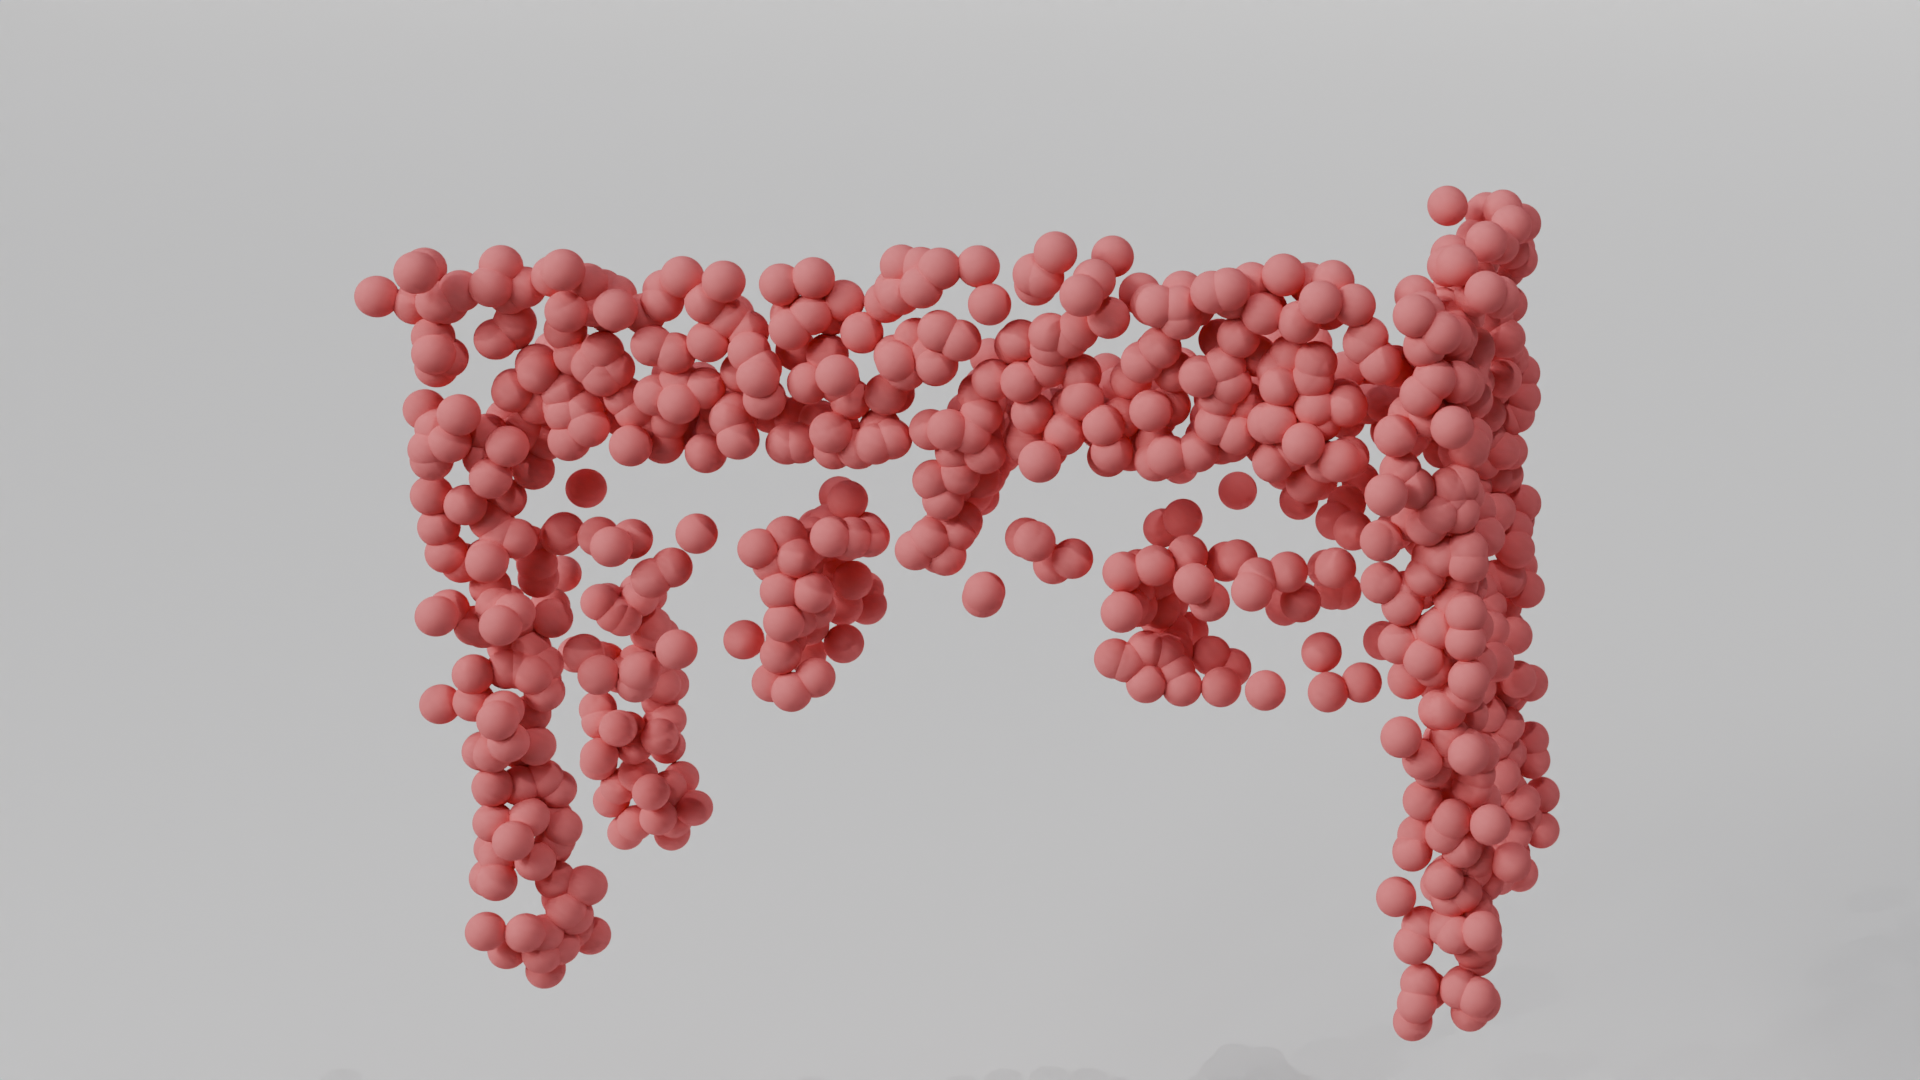
\includegraphics[width=\dimexpr\linewidth-20pt\relax]{figures/part_t1.png}
            \makebox[20pt]{\raisebox{30pt}{\rotatebox[origin=c]{90}{\small DropCon}}}%
            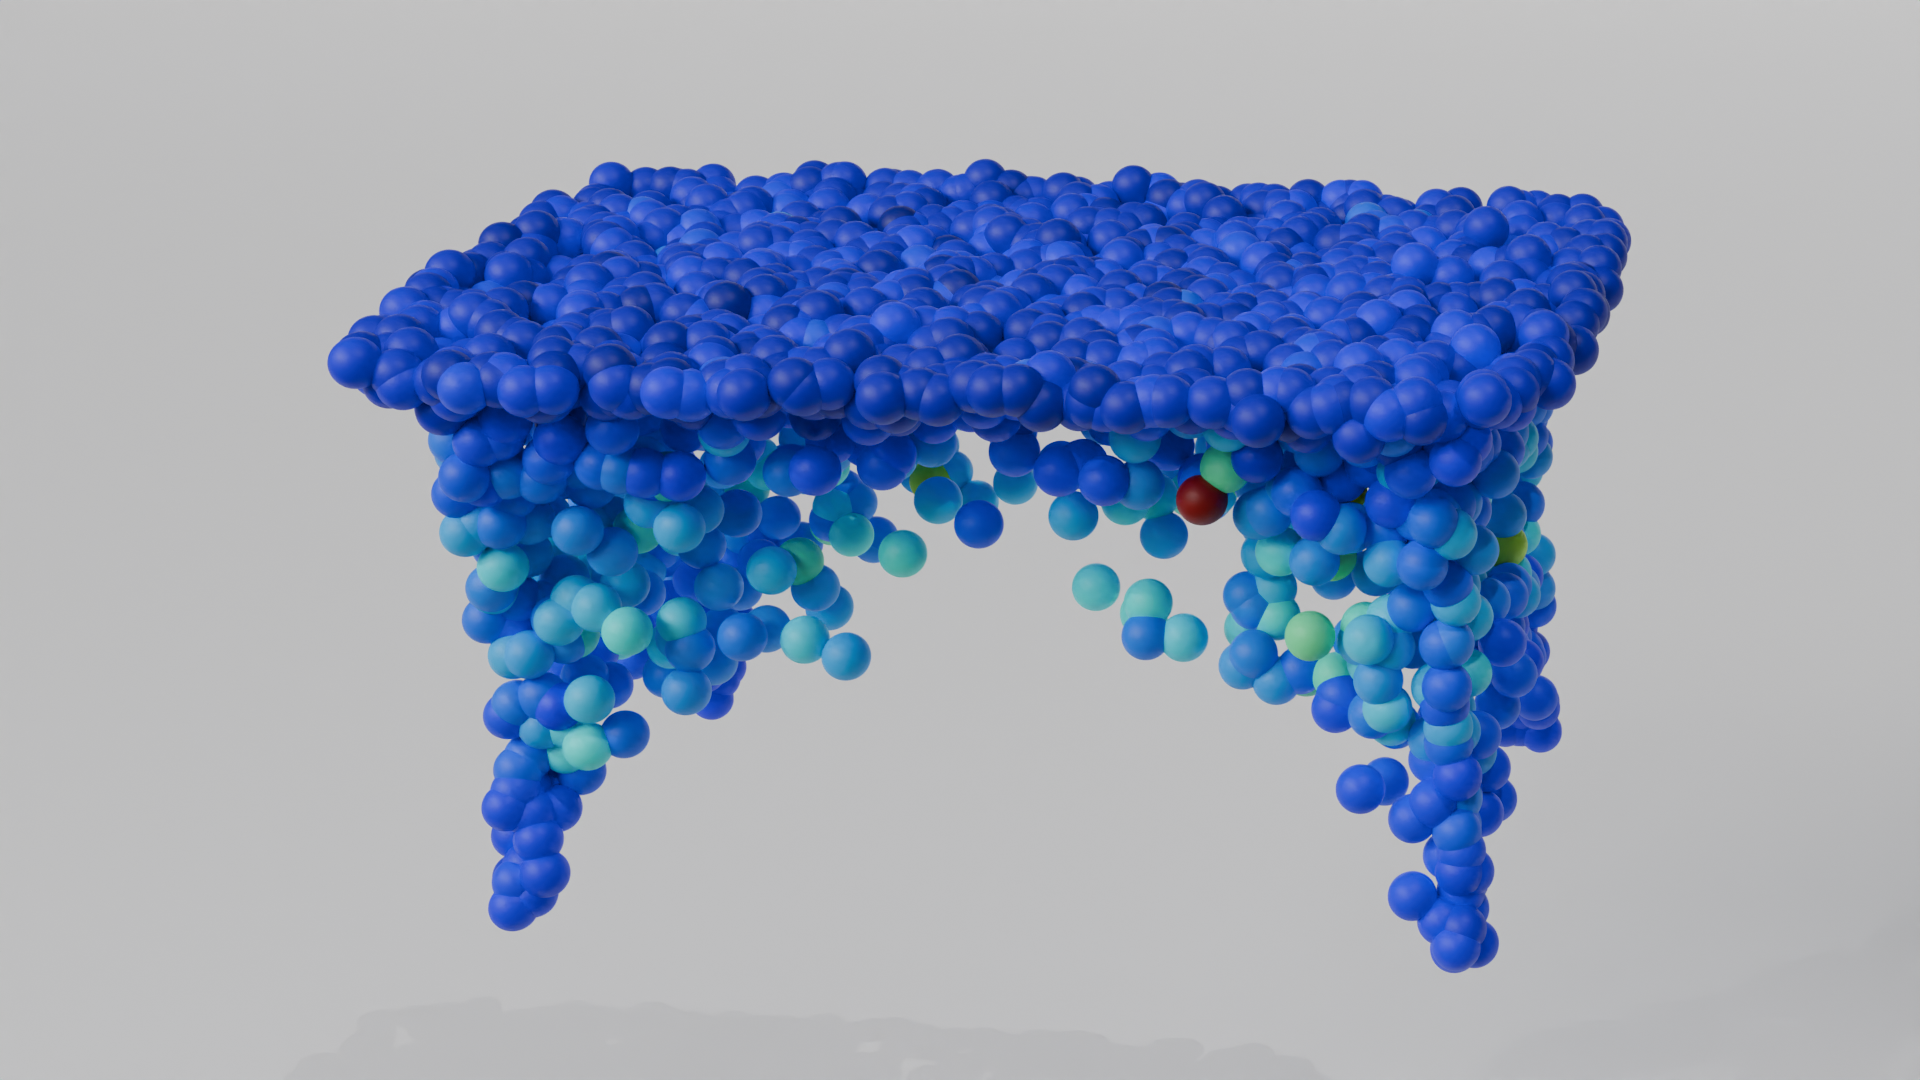
\includegraphics[width=\dimexpr\linewidth-20pt\relax]{figures/dc_lin_t1.png}
            \makebox[20pt]{\raisebox{30pt}{\rotatebox[origin=c]{90}{\small Dropout}}}%
            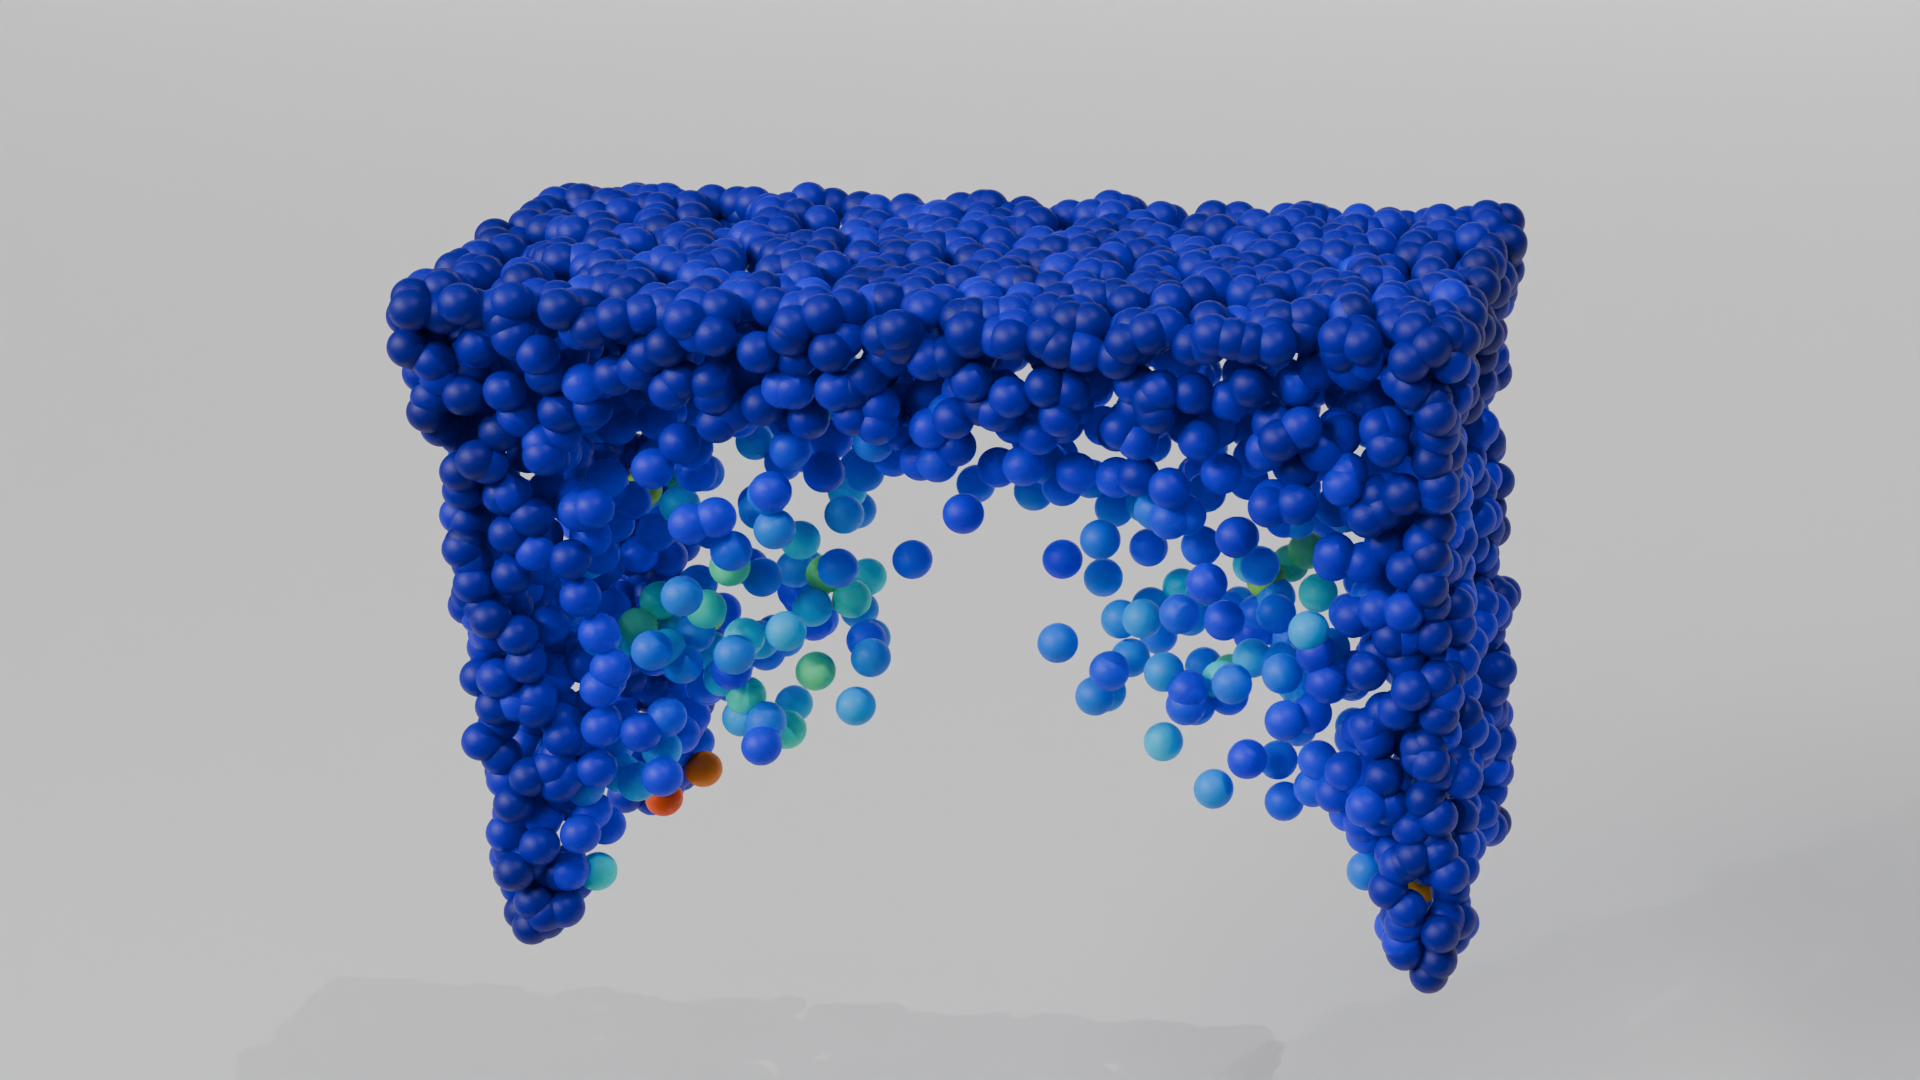
\includegraphics[width=\dimexpr\linewidth-20pt\relax]{figures/do_lin_t1.png}
            \makebox[20pt]{\raisebox{30pt}{\rotatebox[origin=c]{90}{\small Ensemble}}}%
            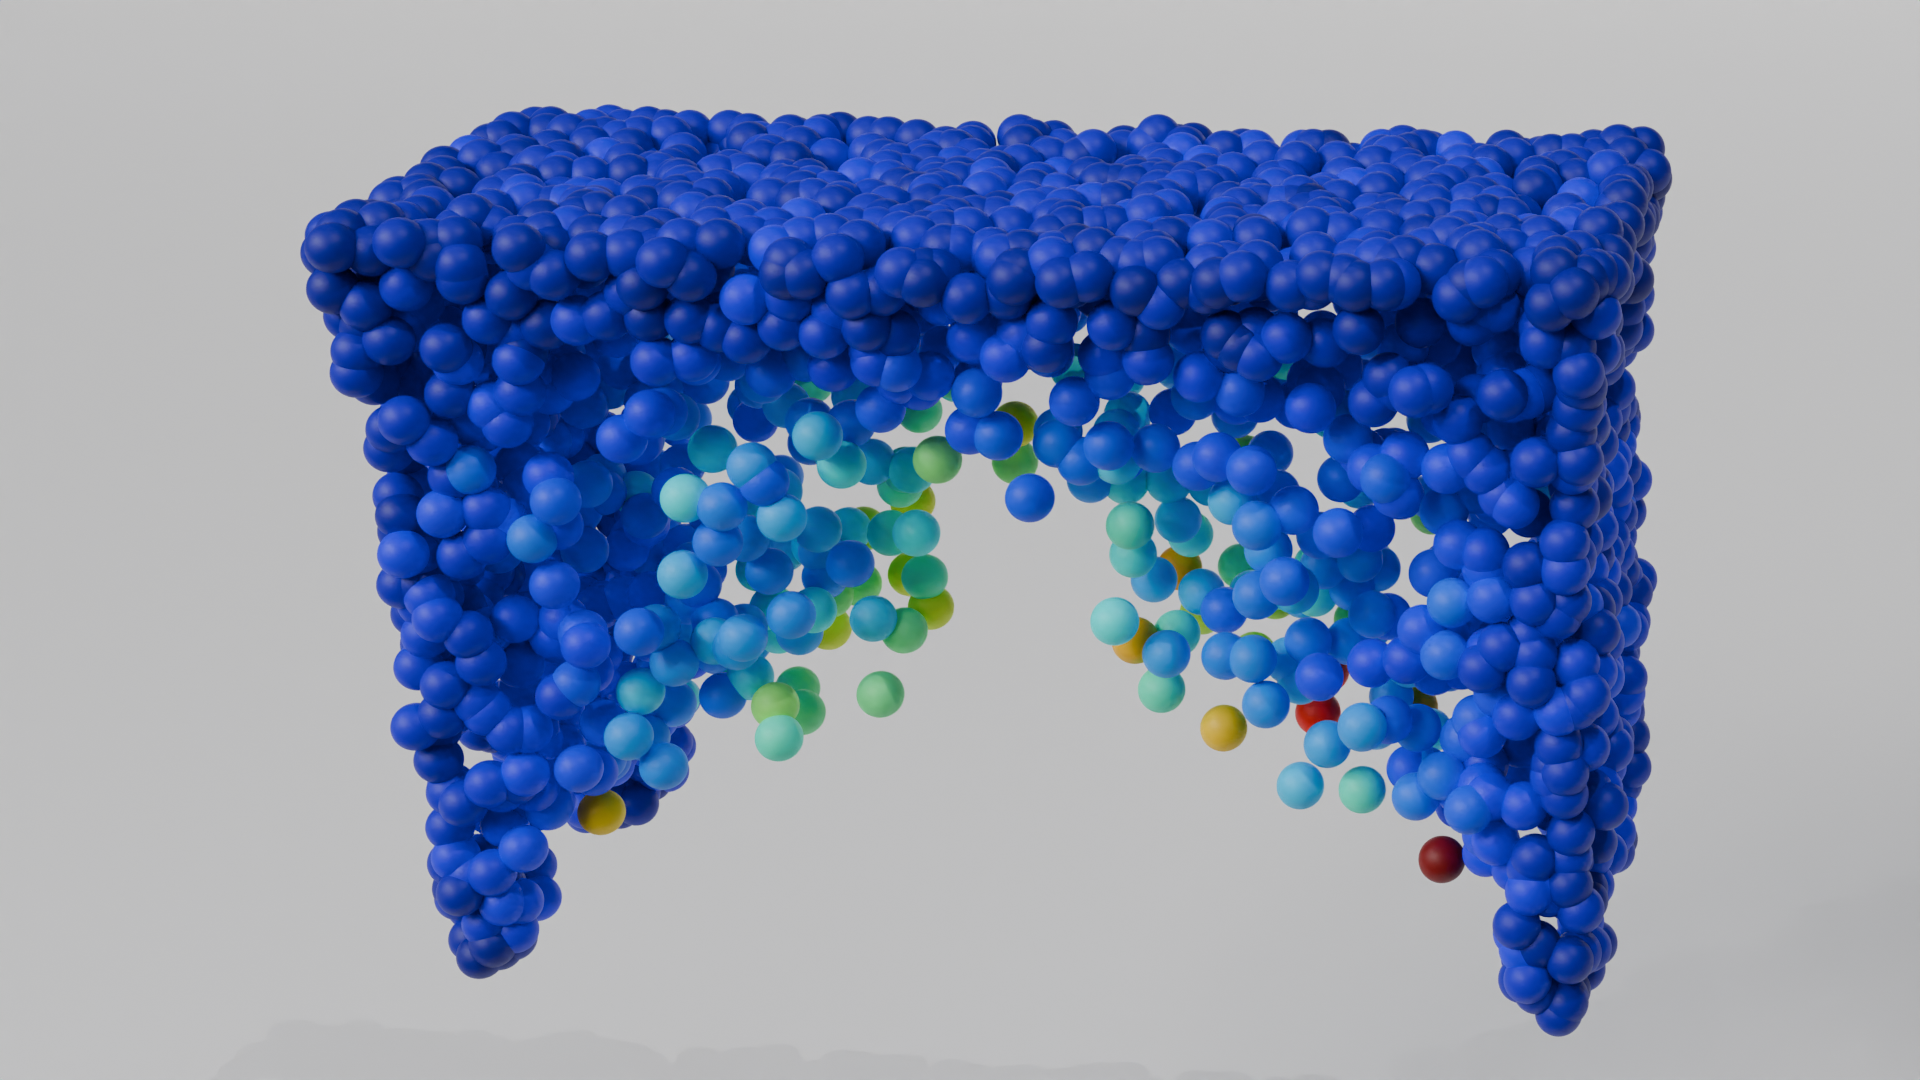
\includegraphics[width=\dimexpr\linewidth-20pt\relax]{figures/ens_lin_t1.png}
            \makebox[20pt]{\raisebox{30pt}{\rotatebox[origin=c]{90}{\small Implicit}}}%
            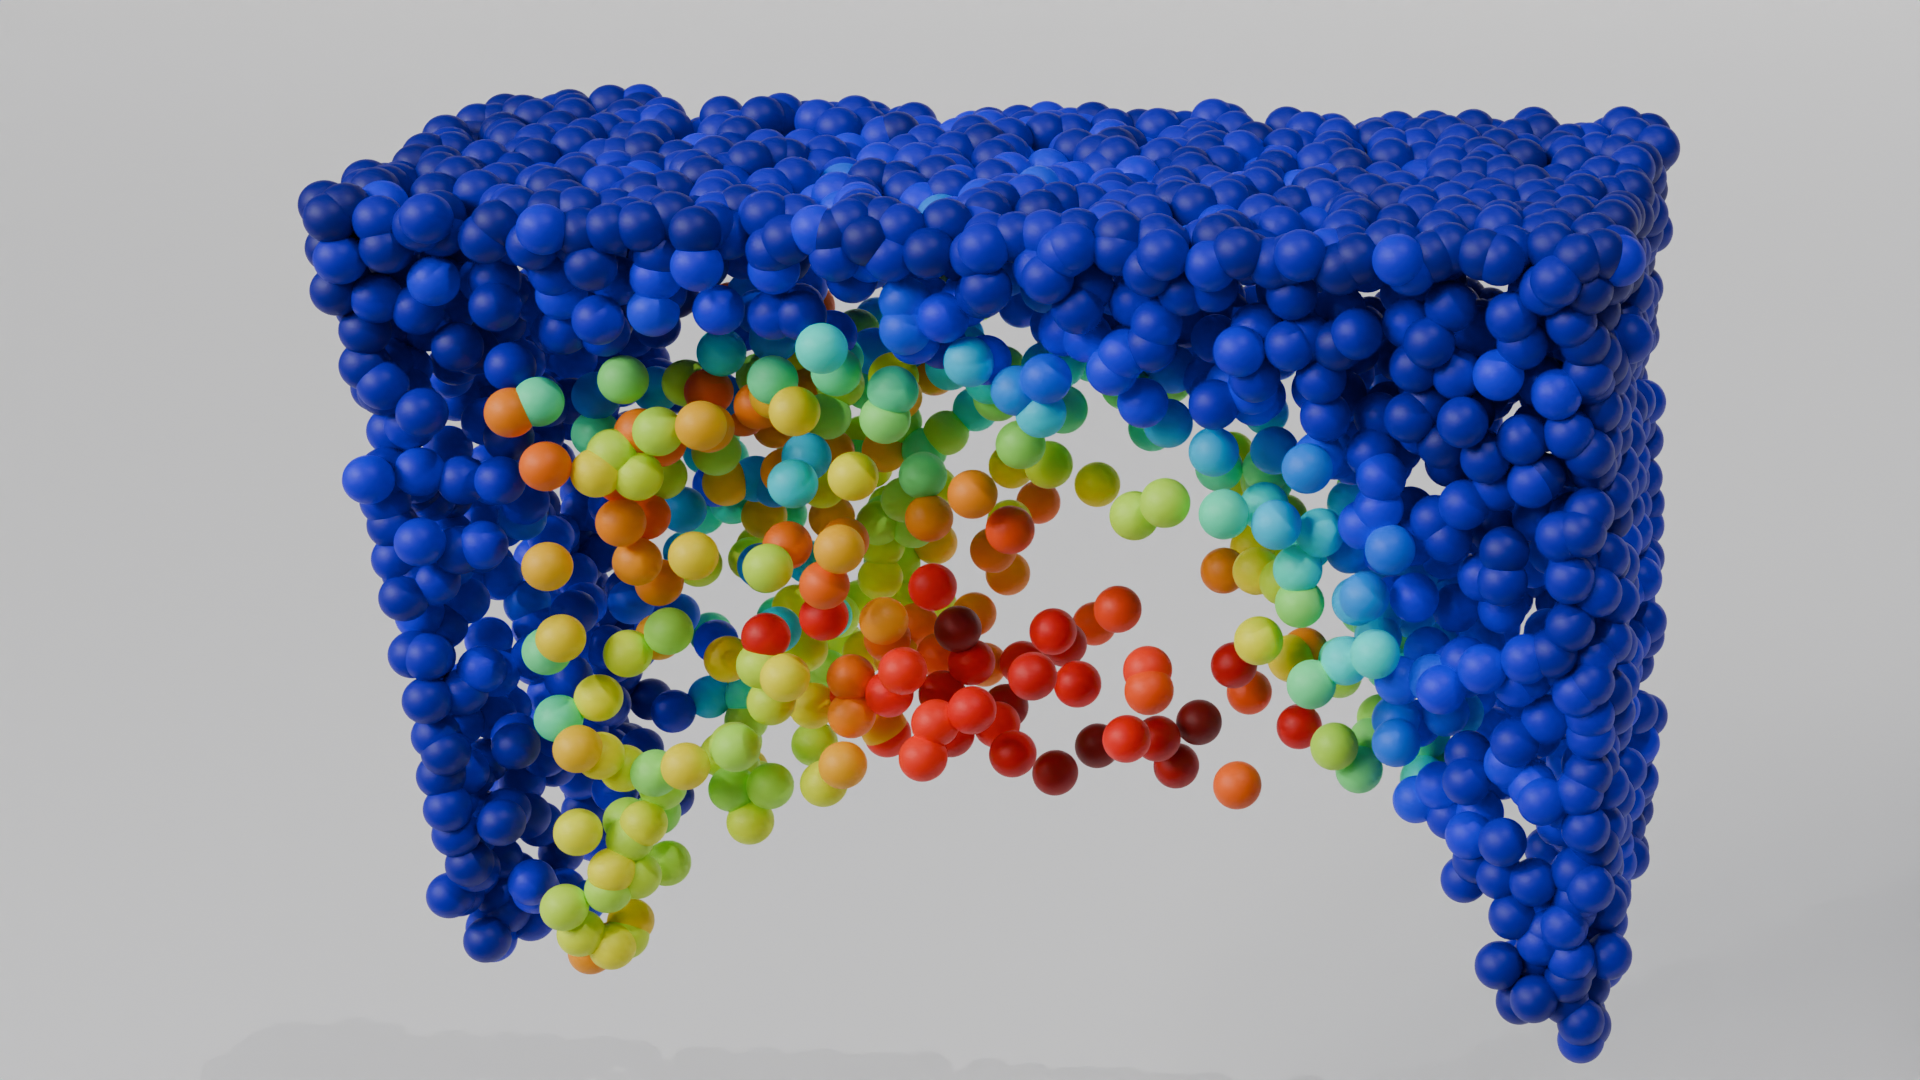
\includegraphics[width=\dimexpr\linewidth-20pt\relax]{figures/iml_lin_t1.png}
            \makebox[20pt]{\raisebox{30pt}{\rotatebox[origin=c]{90}{\small GT}}}%
            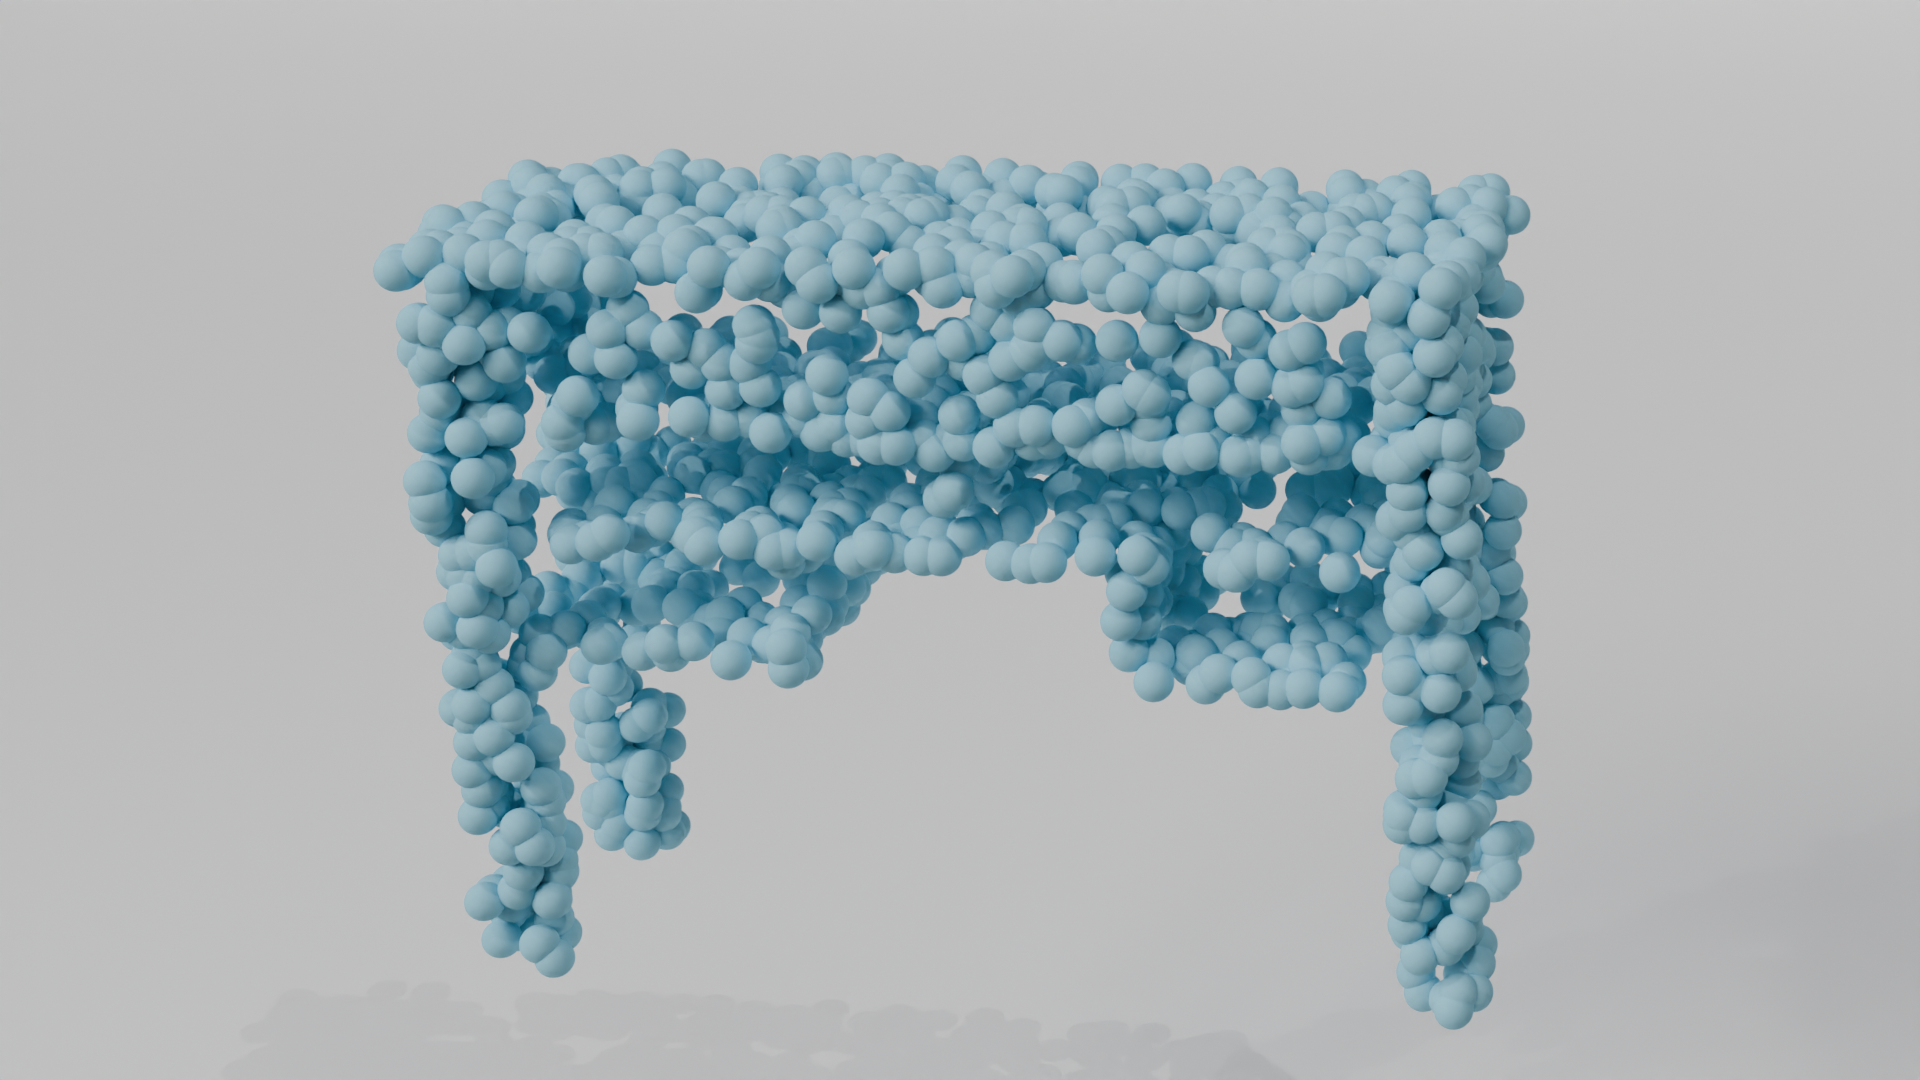
\includegraphics[width=\dimexpr\linewidth-20pt\relax]{figures/com_t1.png}
            \caption{Table 1}
          \end{subfigure}\hfill
          \begin{subfigure}[t]{0.315\textwidth}
            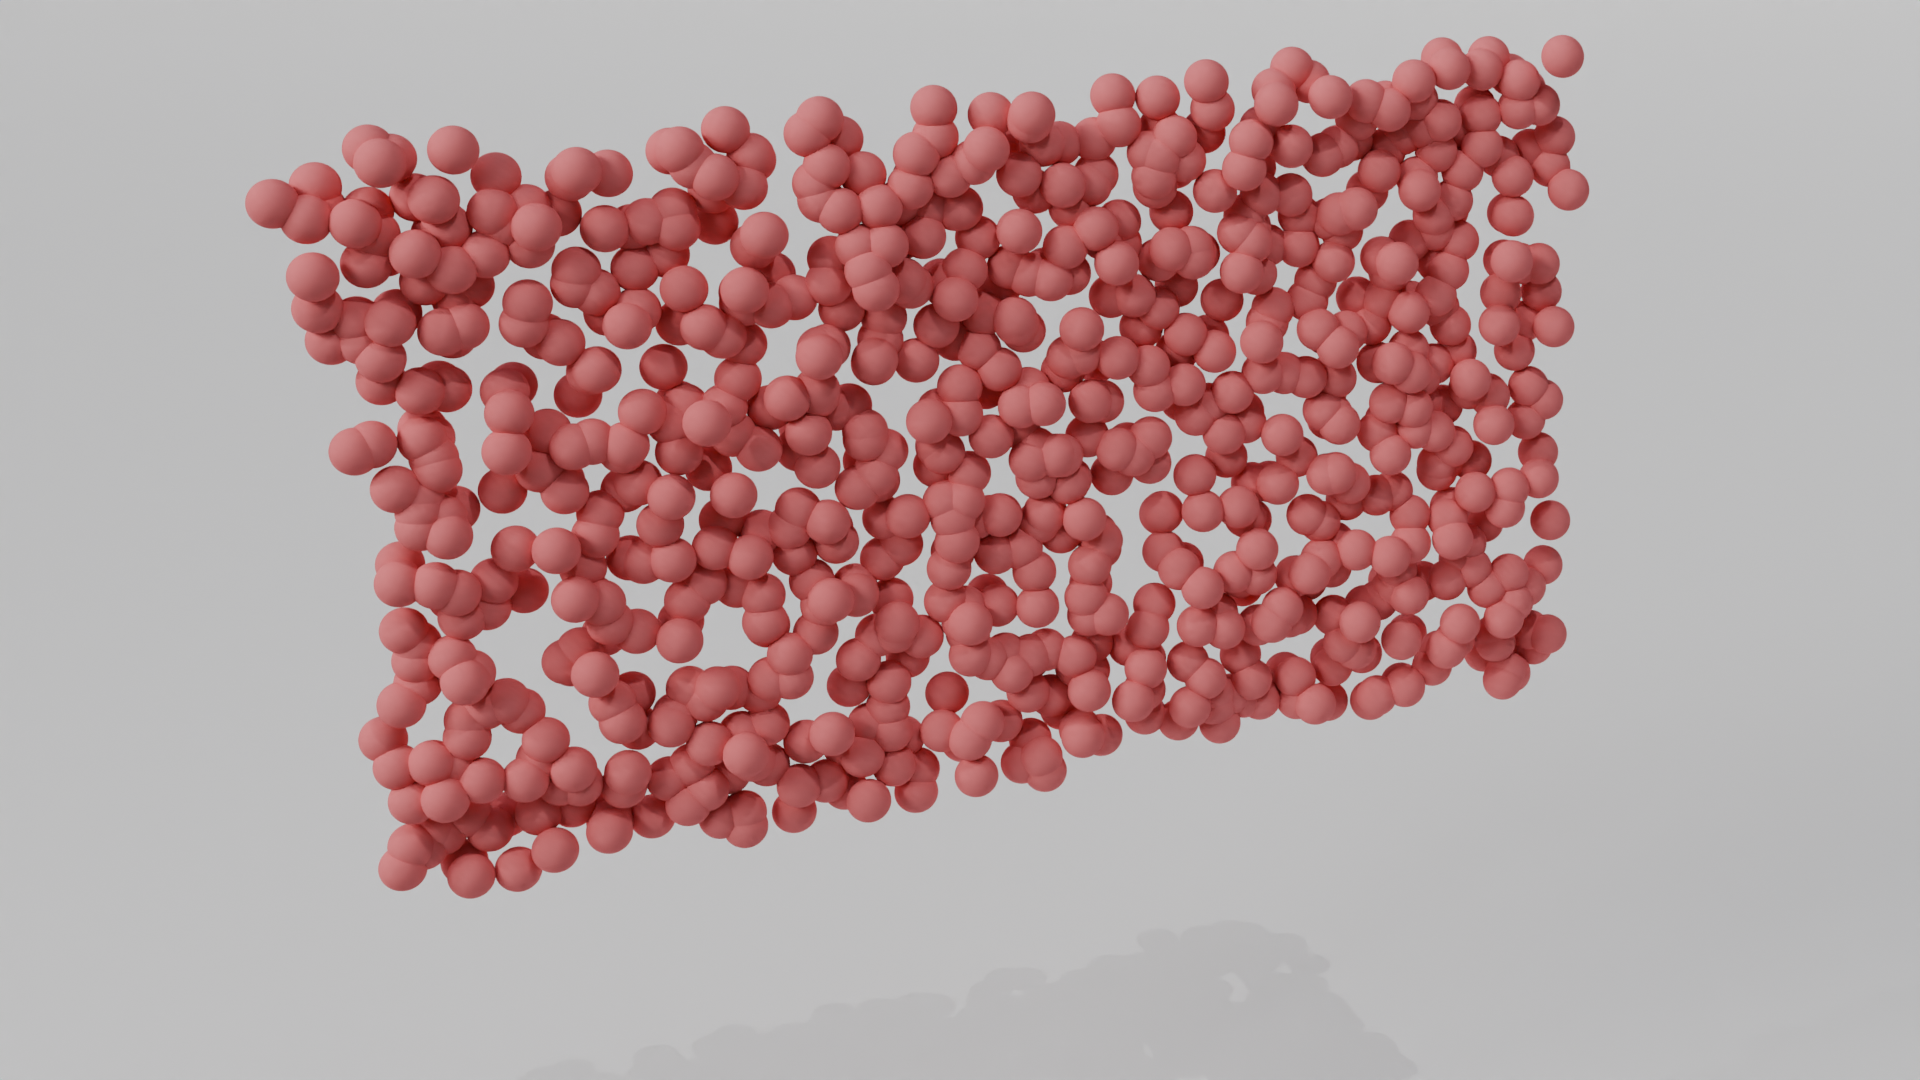
\includegraphics[width=\textwidth]{figures/part_t2.png}
            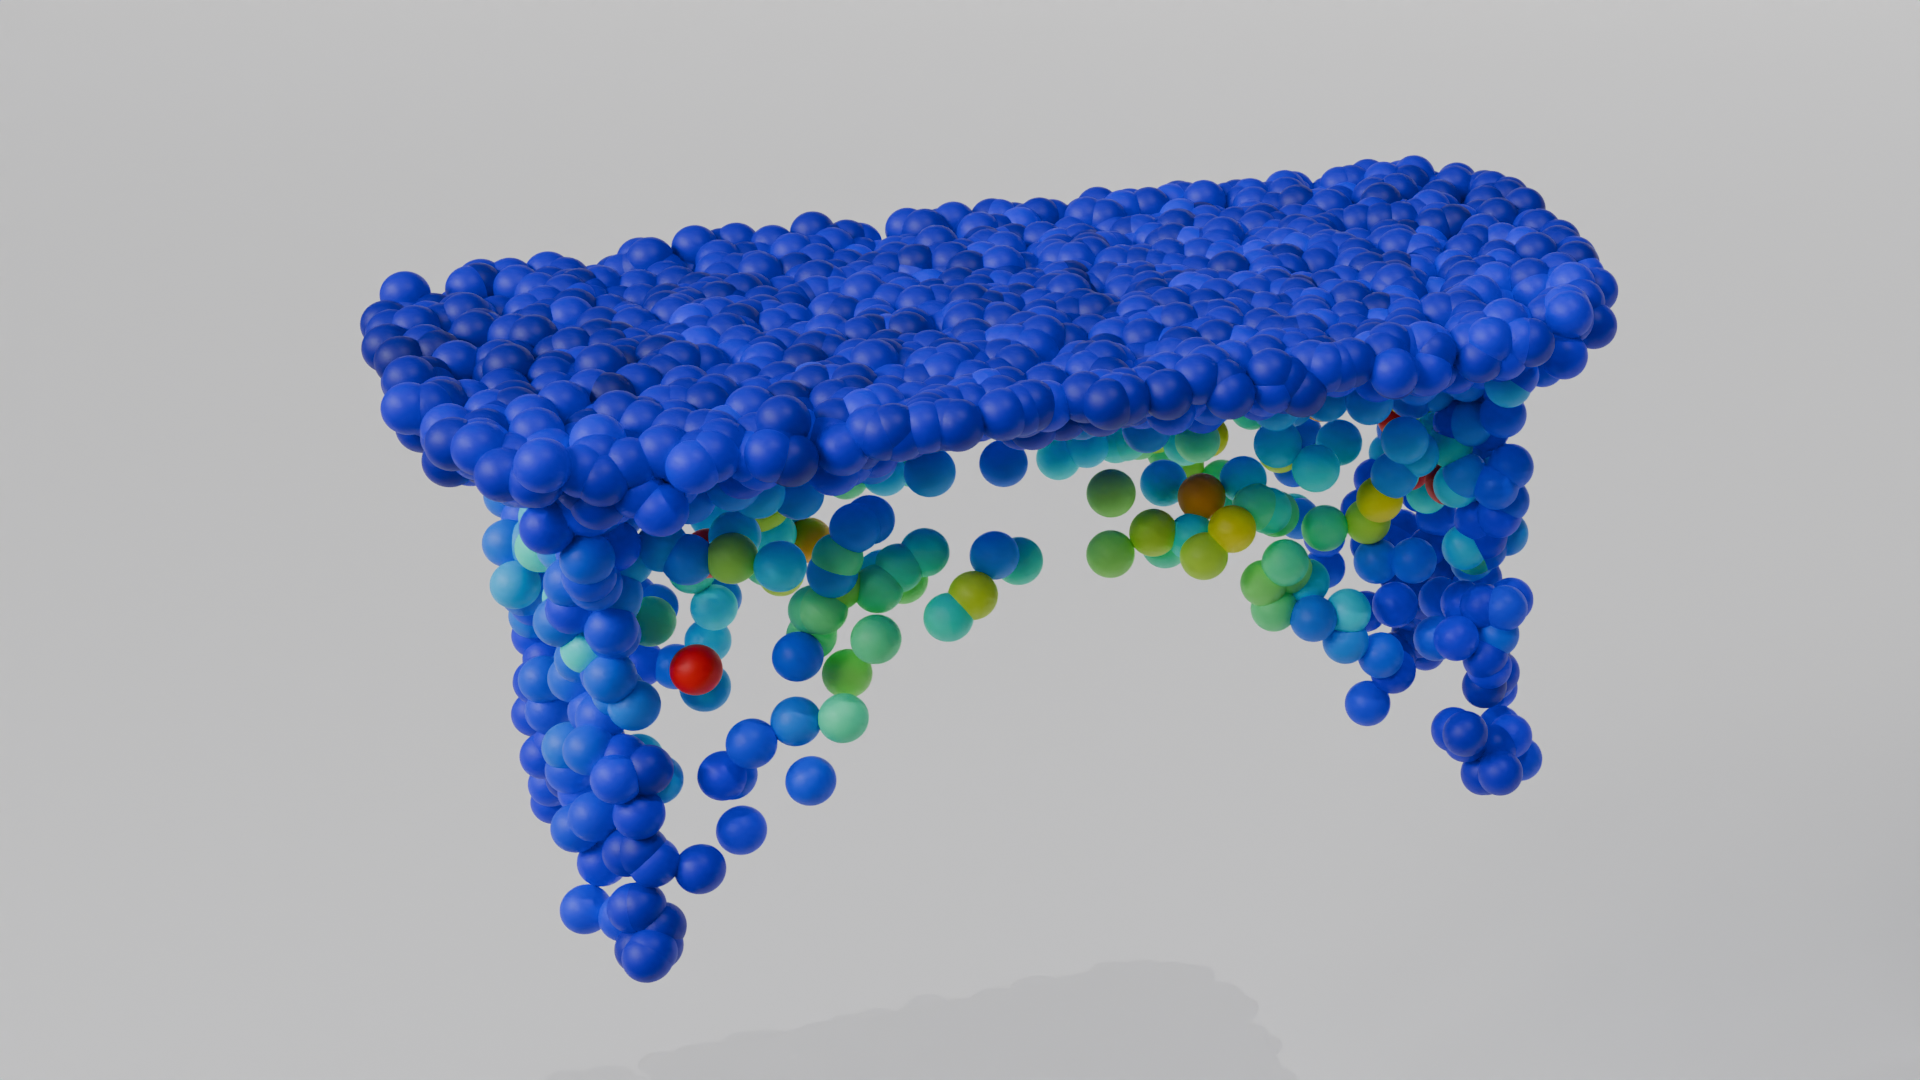
\includegraphics[width=\textwidth]{figures/dc_lin_t2.png}
            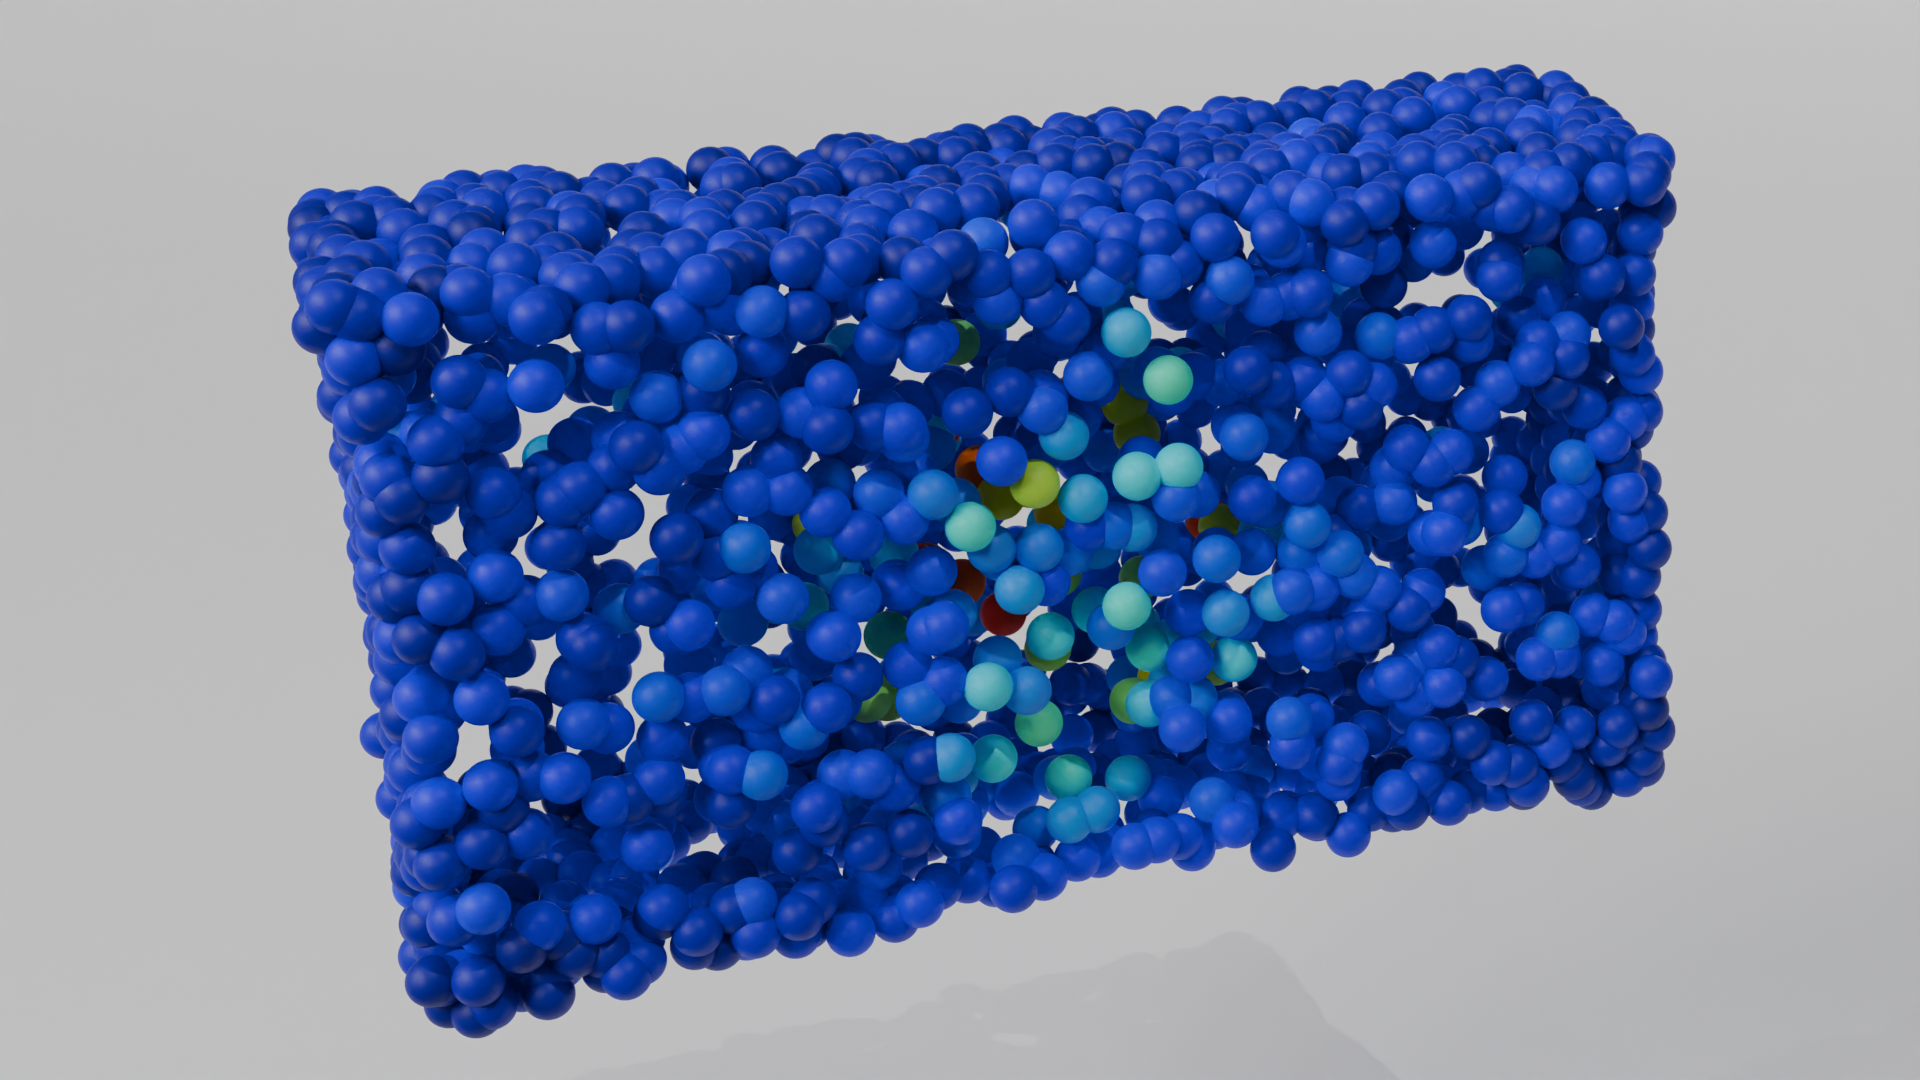
\includegraphics[width=\textwidth]{figures/do_lin_t2.png}
            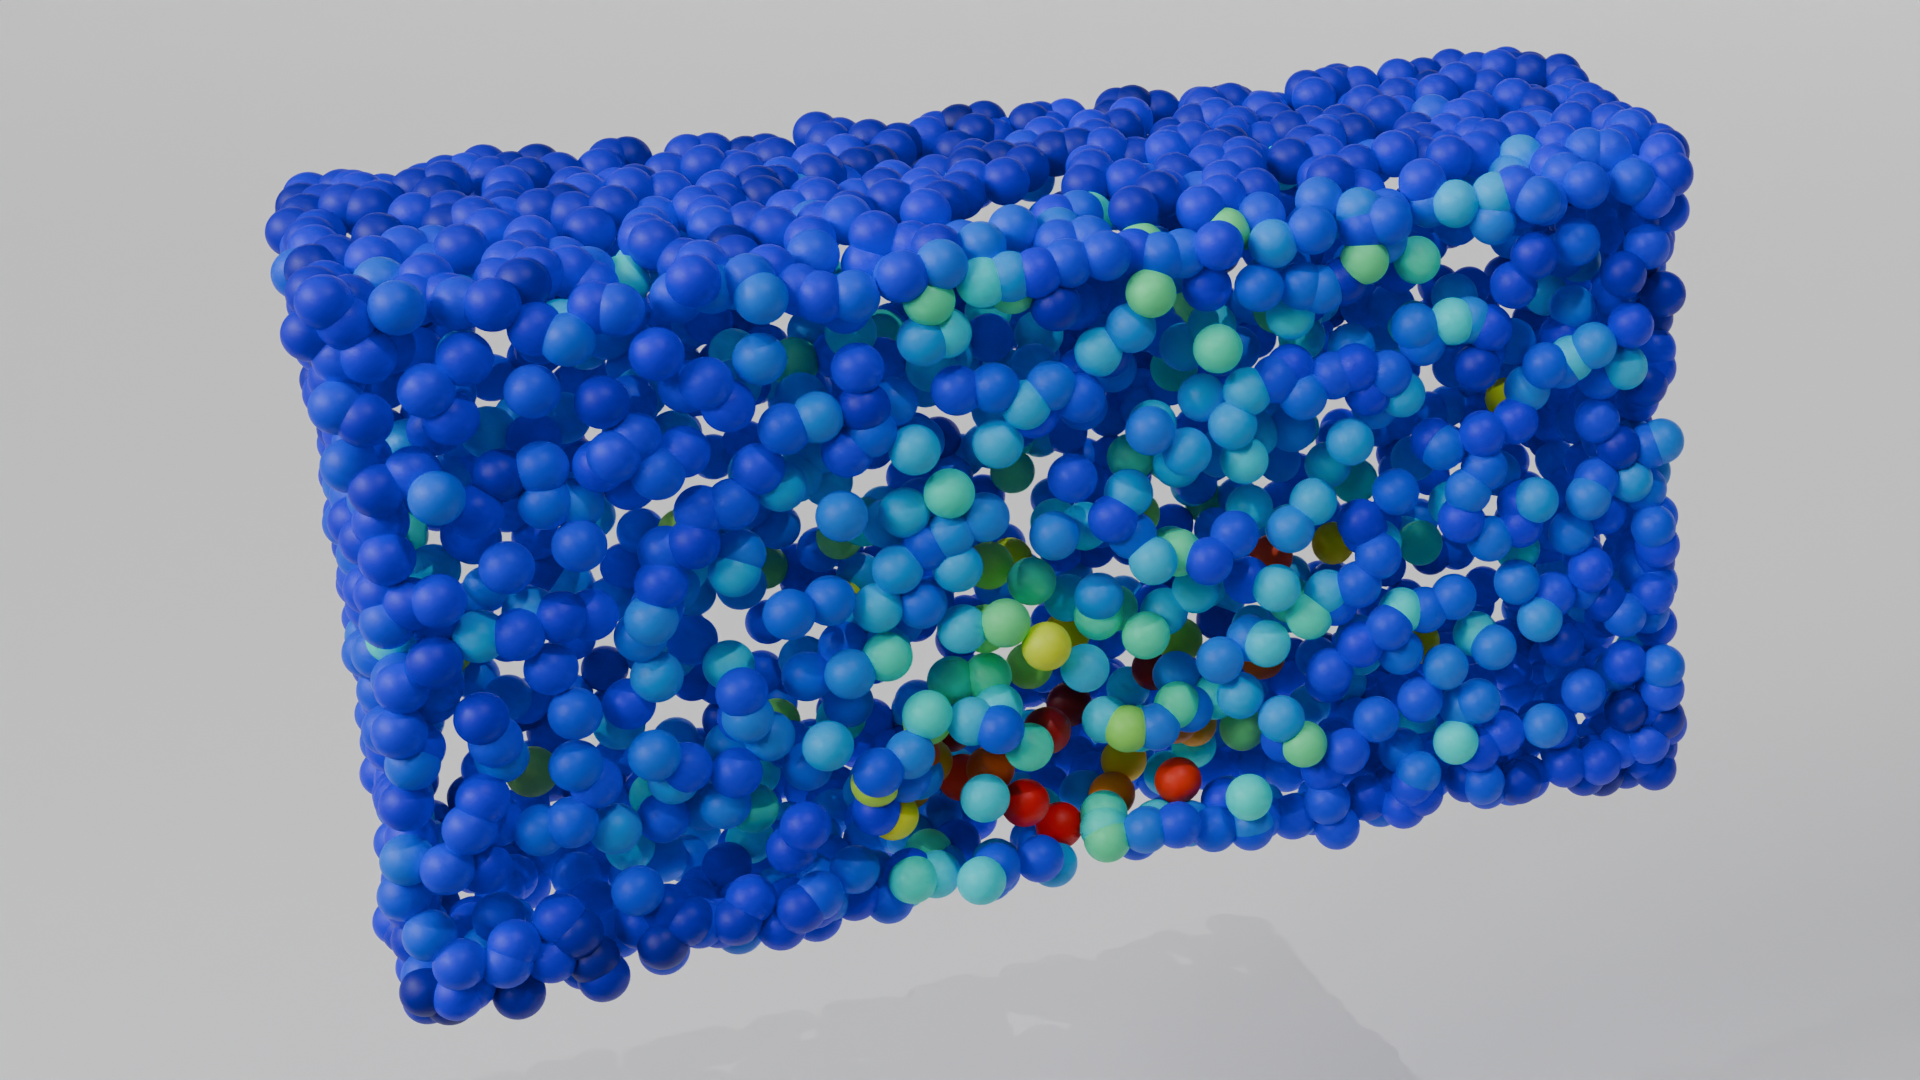
\includegraphics[width=\textwidth]{figures/ens_lin_t2.png}
            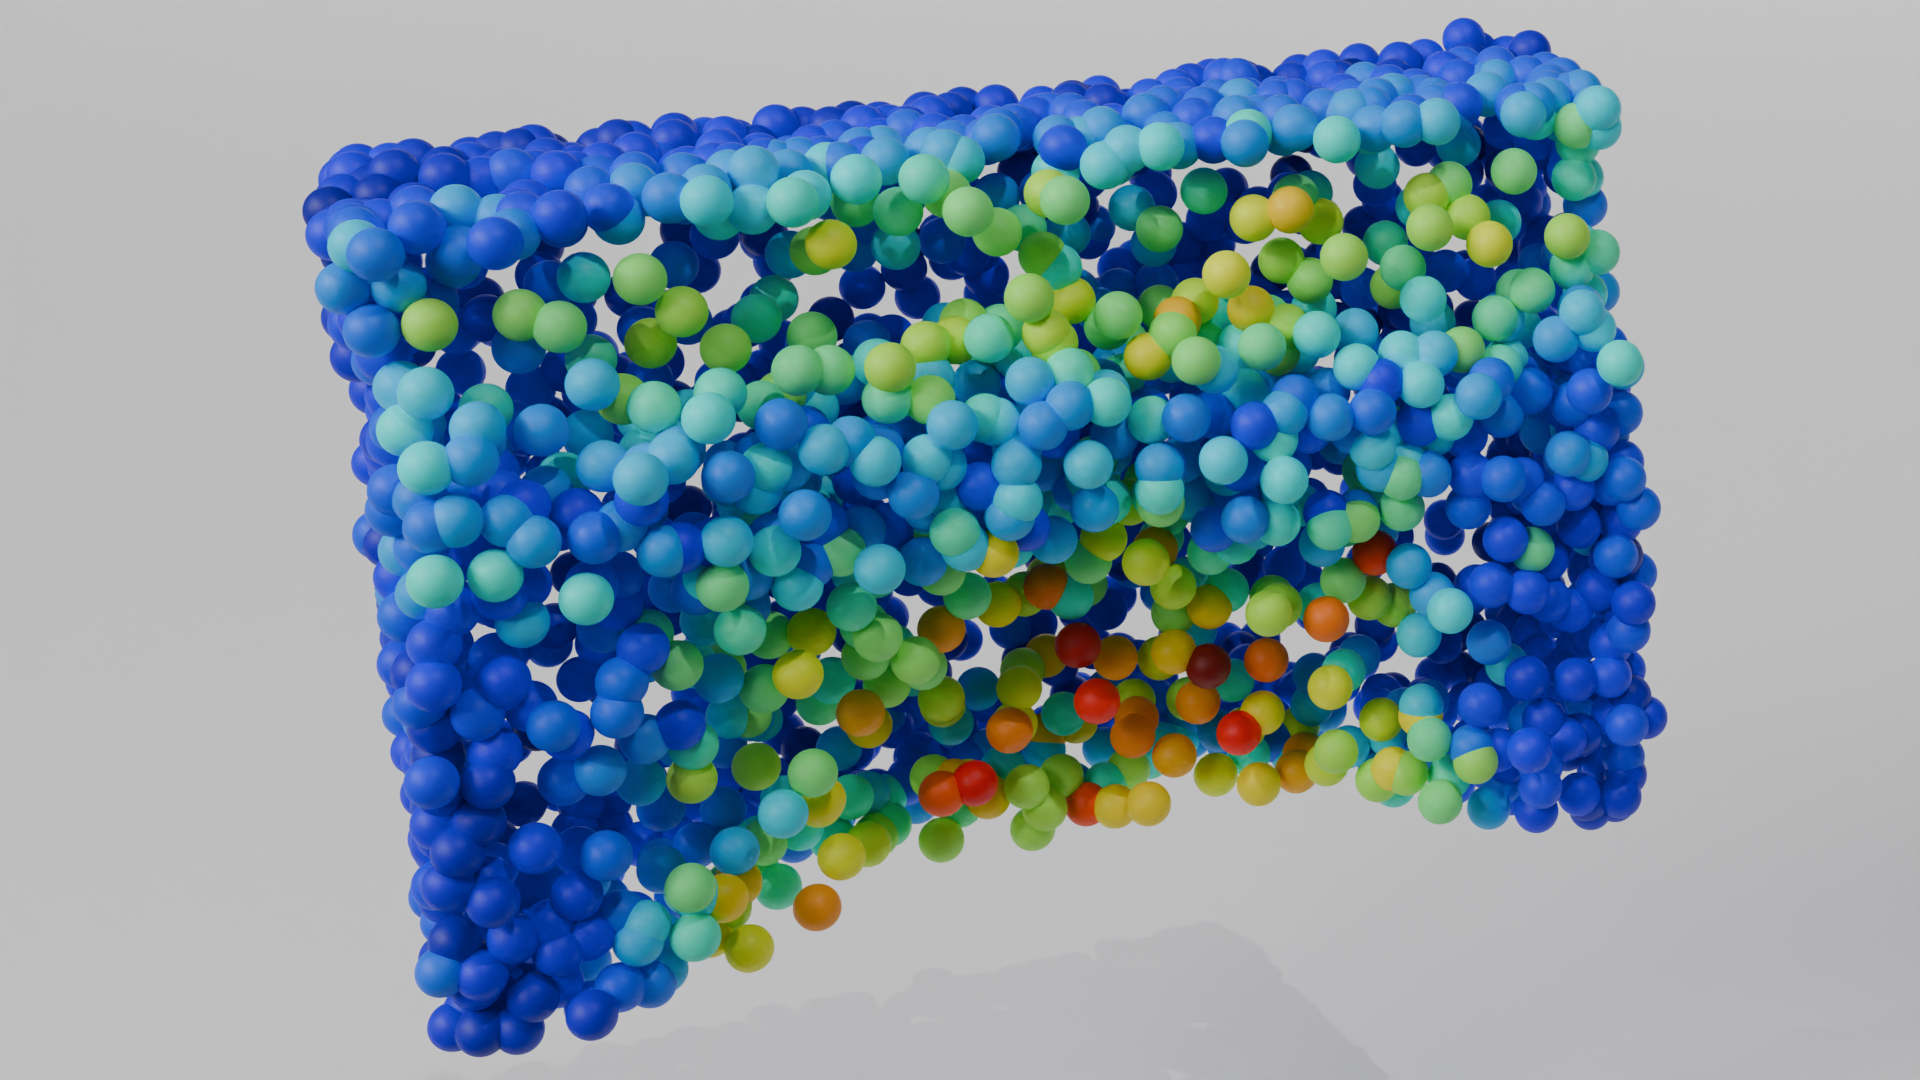
\includegraphics[width=\textwidth]{figures/iml_lin_t2.png}
            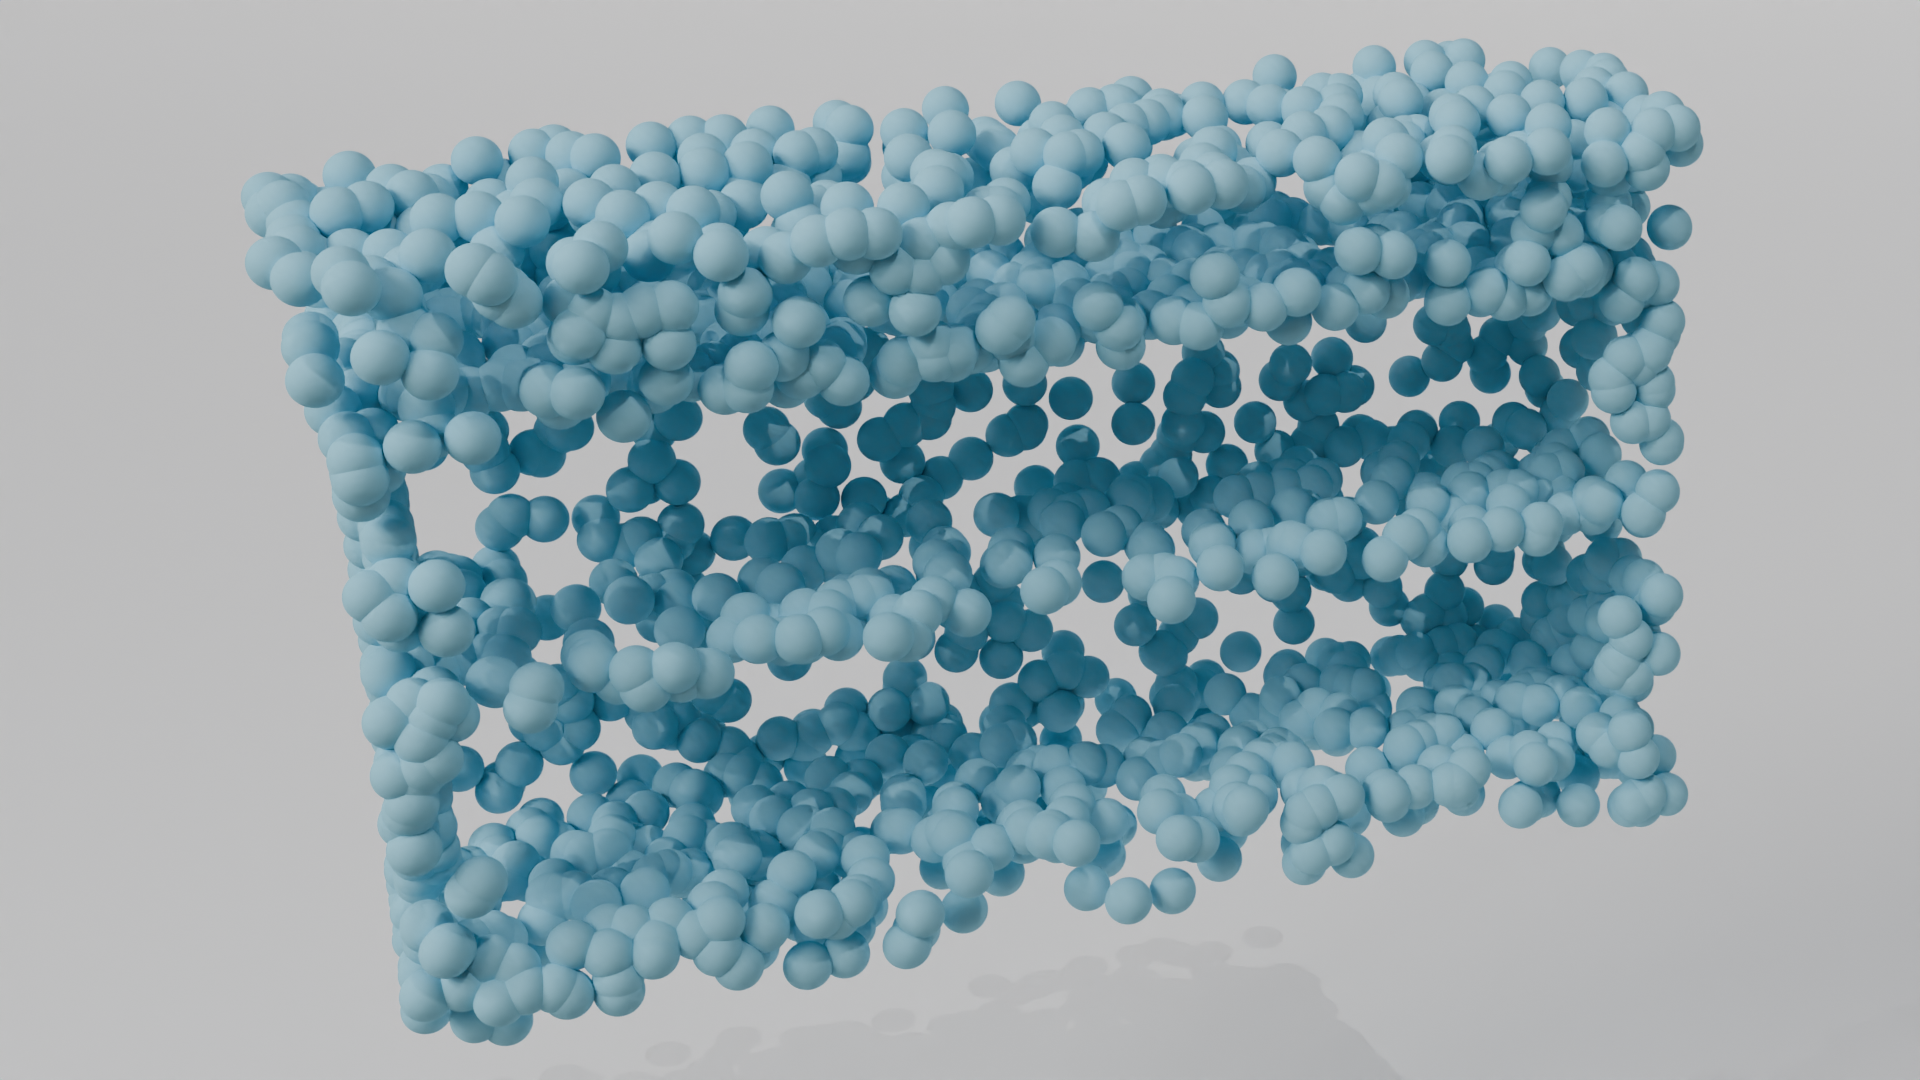
\includegraphics[width=\textwidth]{figures/com_t2.png}
            \caption{Table 2}
          \end{subfigure}\hfill
          \begin{subfigure}[t]{0.315\textwidth}
            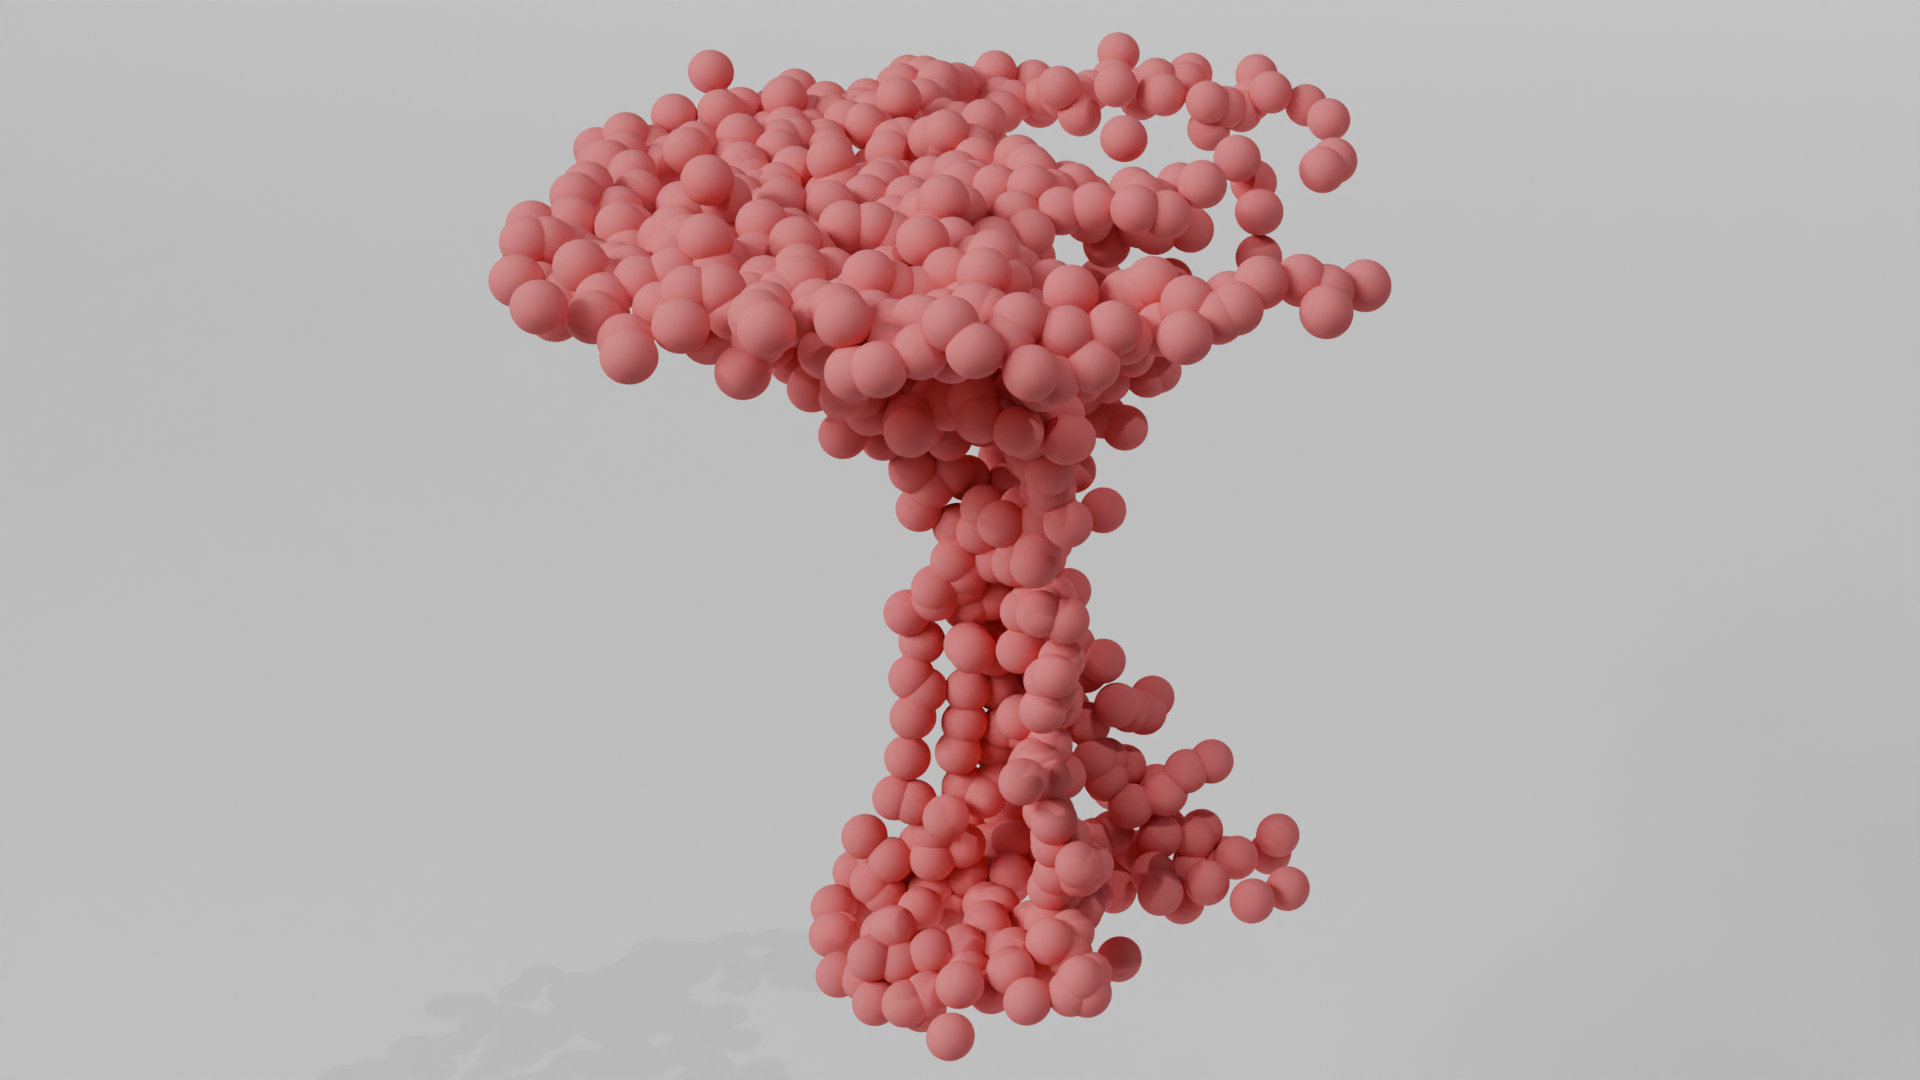
\includegraphics[width=\textwidth]{figures/part_t3.png}
            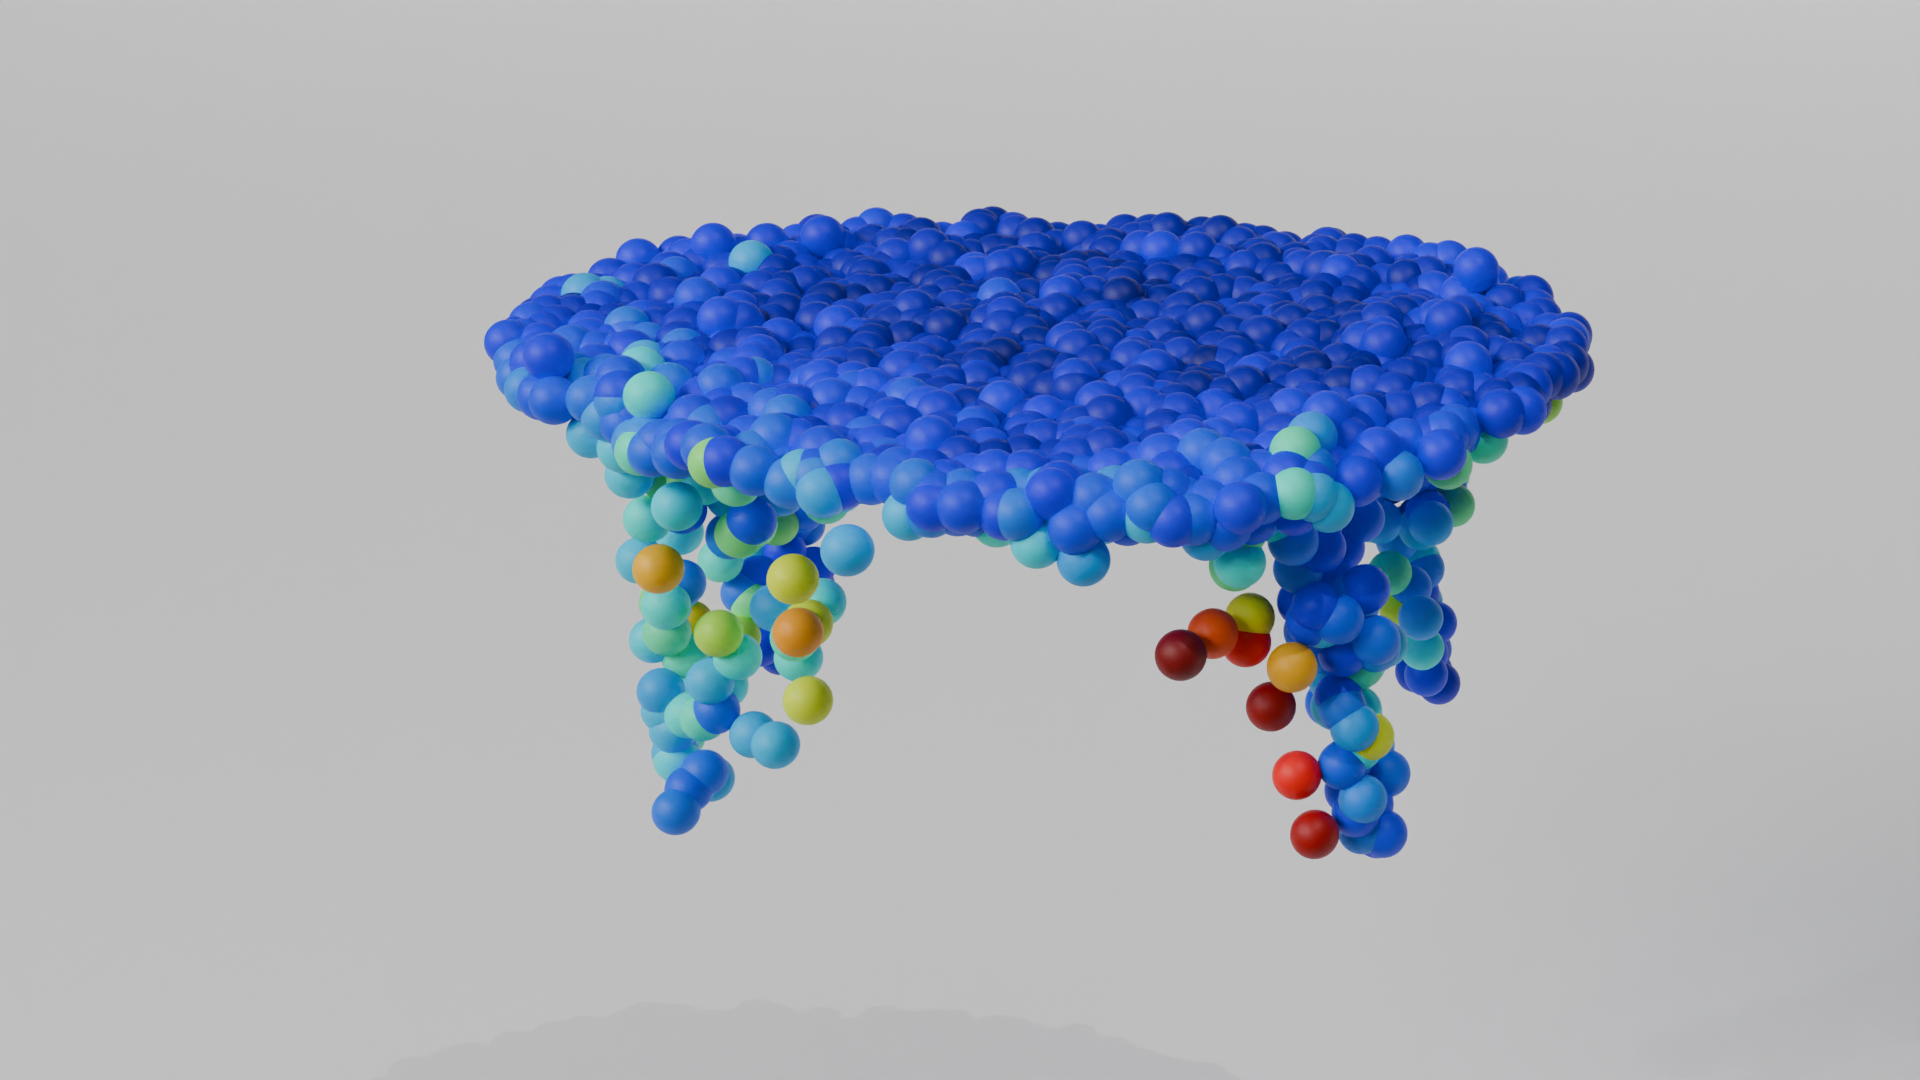
\includegraphics[width=\textwidth]{figures/dc_lin_t3.png}
            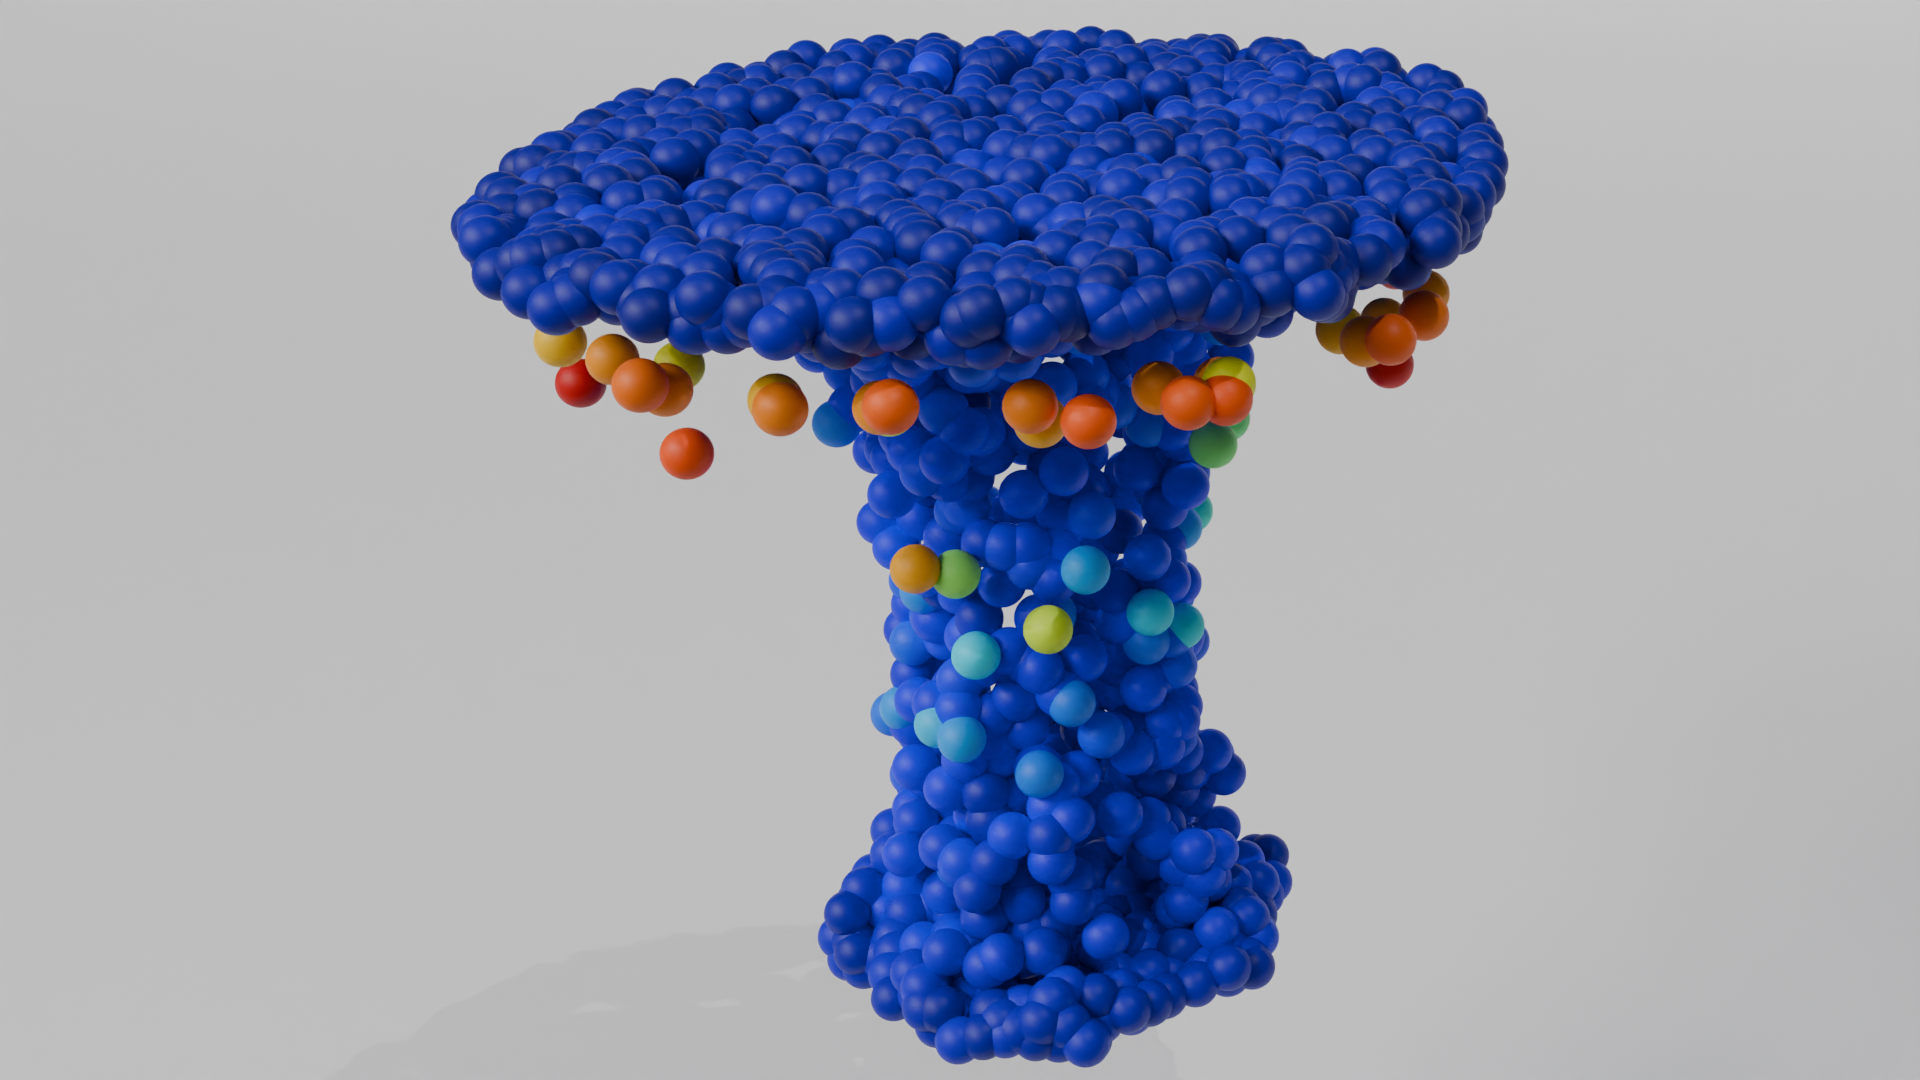
\includegraphics[width=\textwidth]{figures/do_lin_t3.png}
            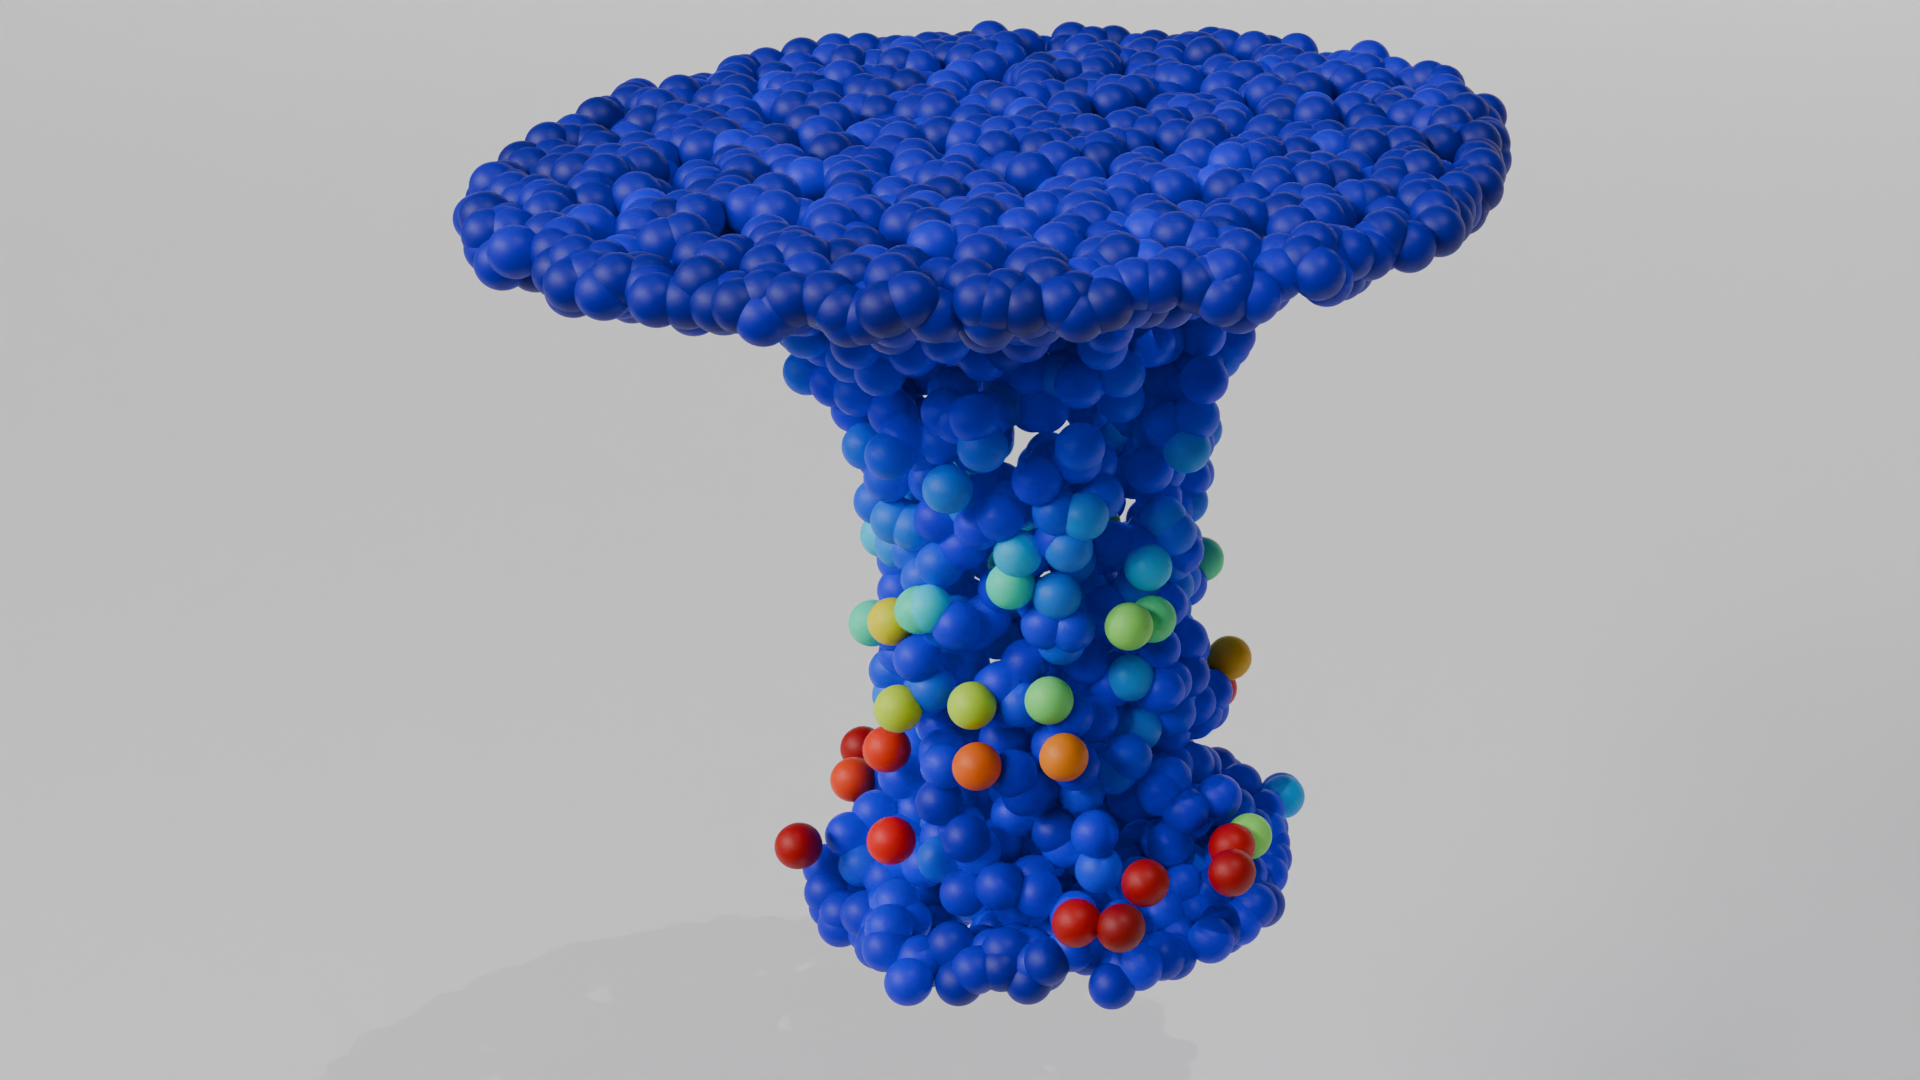
\includegraphics[width=\textwidth]{figures/ens_lin_t3.png}
            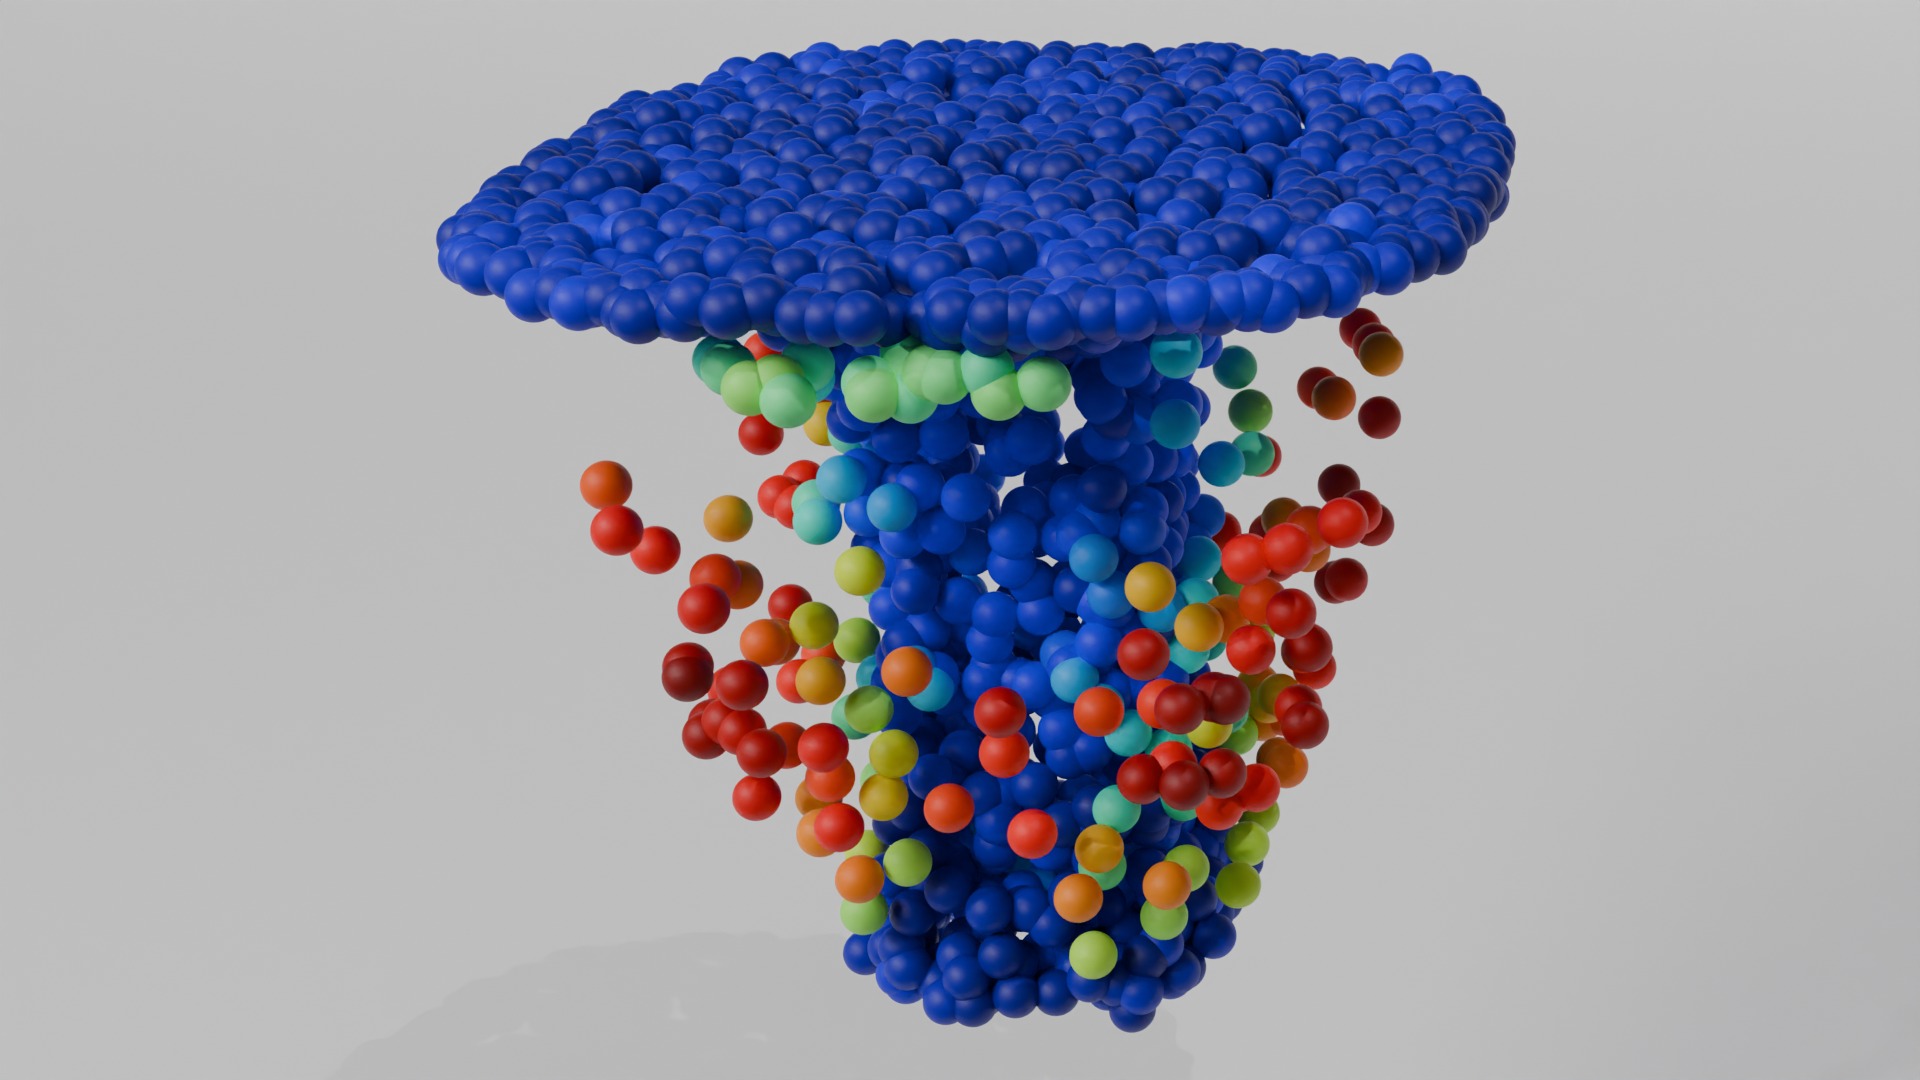
\includegraphics[width=\textwidth]{figures/iml_lin_t3.png}
            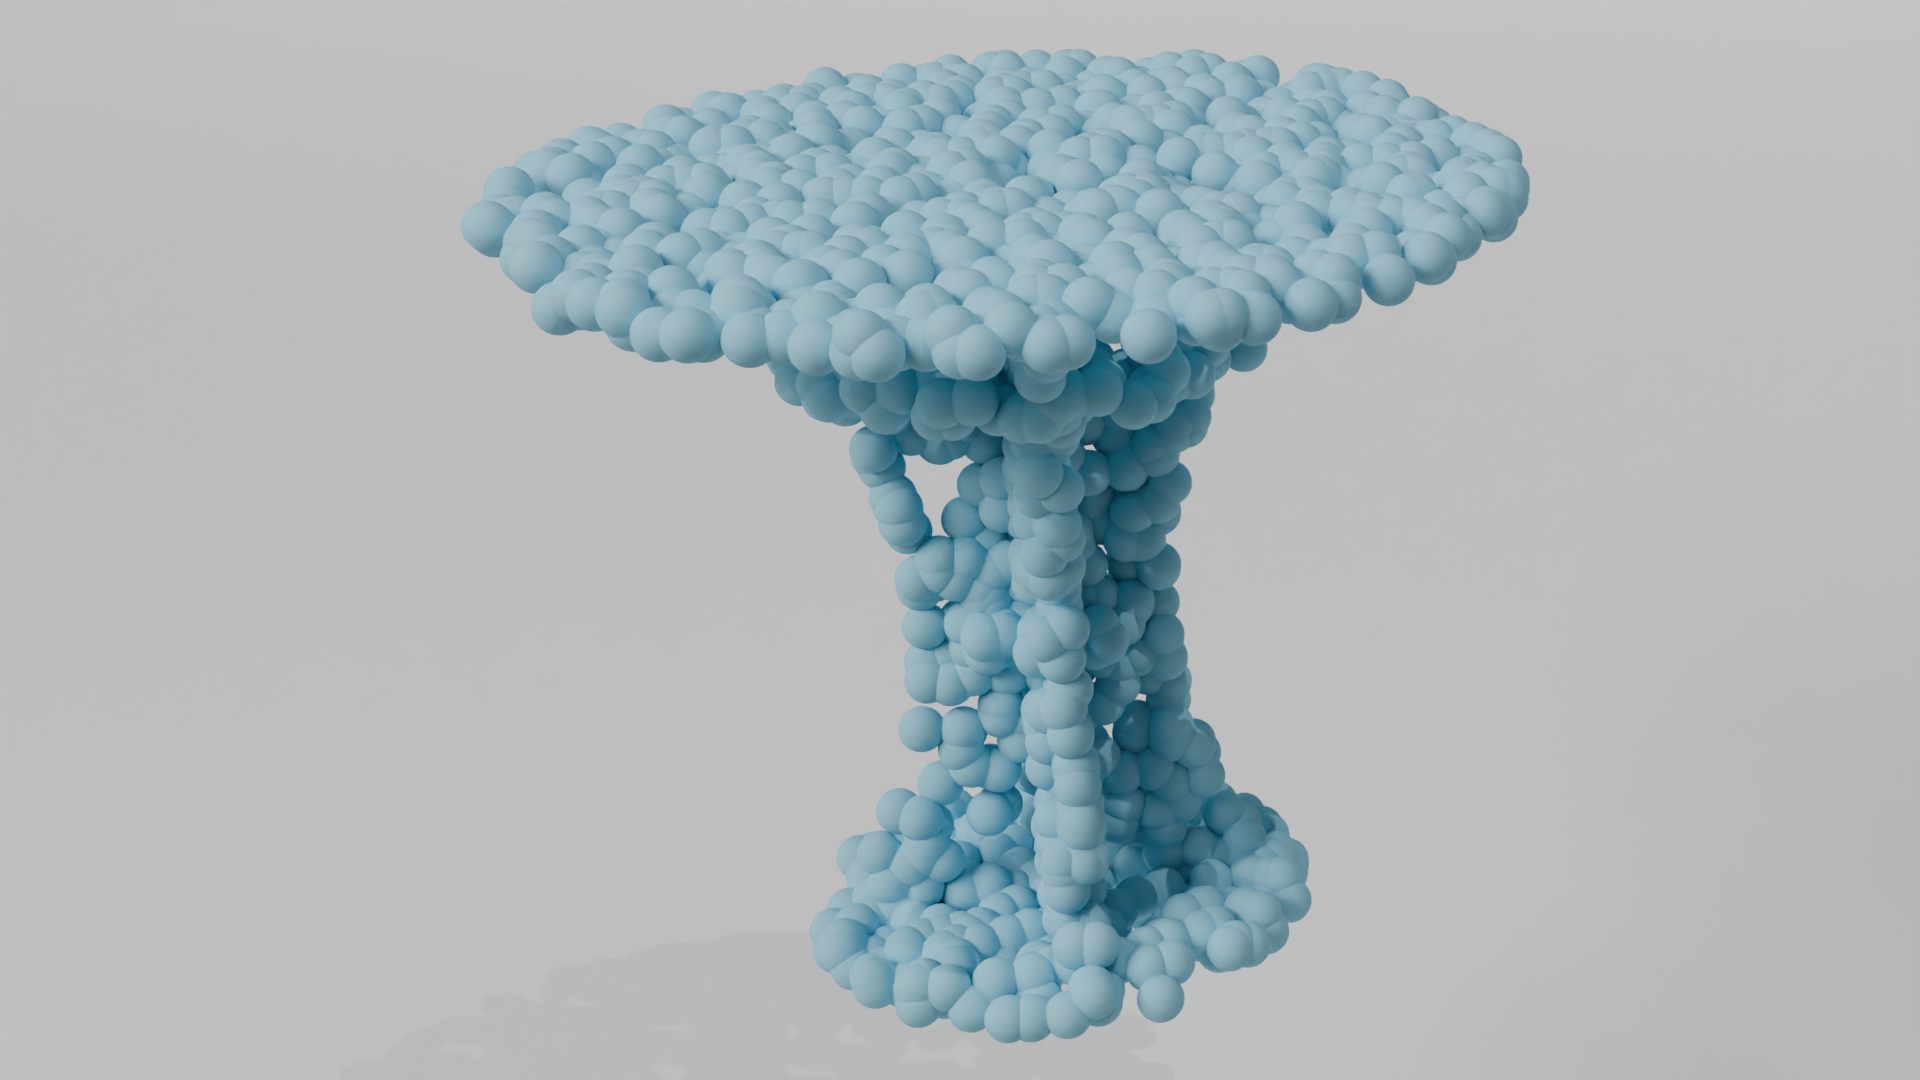
\includegraphics[width=\textwidth]{figures/com_t3.png}
            \caption{Table 3}
          \end{subfigure}
          \caption{Qualitative comparison between different empirical uncertainty quantification methods for point cloud completion on the table subcategory of ShapeNet data. Input refers to the partial point cloud, and GT refers to the ground truth complete cloud. DropCon, Dropout, Ensemble, and Implicit refer to the uncertainty maps output by the DropConnect, dropout, deep ensemble, and implicit generative model-based methods, respectively.}
          \label{fig:table}
        \end{figure}

        \subsubsection{Effect of Number of Generated Samples}
        A comparison between the uncertainty maps produced by different numbers of generated clouds is shown in Figure~\ref{fig:zairplanezz} for a randomly selected example from the airplane subcategory of ShapeNet data. For each input, 5, 10, 25, and 50 different completions were produced for three methods, and uncertainty maps were computed using linear assignment matching between the generated clouds. Ensemble-based methods were ignored due to the computational cost and the memory required to store the models.
        \begin{figure}[htb]
          \centering
          \begin{subfigure}[t]{\dimexpr0.315\textwidth+20pt\relax}
            \makebox[20pt]{\raisebox{30pt}{\rotatebox[origin=c]{90}{\small Input}}}%
            \includegraphics[width=\dimexpr\linewidth-20pt\relax]{figures/part_ap.png}
            \makebox[20pt]{\raisebox{30pt}{\rotatebox[origin=c]{90}{\small $M$=5}}}%
            \includegraphics[width=\dimexpr\linewidth-20pt\relax]{figures/5z_ap_mcdc.png}
            \makebox[20pt]{\raisebox{30pt}{\rotatebox[origin=c]{90}{\small $M$=10}}}%
            \includegraphics[width=\dimexpr\linewidth-20pt\relax]{figures/10z_ap_mcdc.png}
            \makebox[20pt]{\raisebox{30pt}{\rotatebox[origin=c]{90}{\small $M$=25}}}%
            \includegraphics[width=\dimexpr\linewidth-20pt\relax]{figures/25z_ap_mcdc.png}
            \makebox[20pt]{\raisebox{30pt}{\rotatebox[origin=c]{90}{\small $M$=50}}}%
            \includegraphics[width=\dimexpr\linewidth-20pt\relax]{figures/50z_ap_mcdc.png}
            \makebox[20pt]{\raisebox{30pt}{\rotatebox[origin=c]{90}{\small GT}}}%
            \includegraphics[width=\dimexpr\linewidth-20pt\relax]{figures/comp_ap.png}
            \caption{MC DropConnect}
          \end{subfigure}\hfill
          \begin{subfigure}[t]{0.315\textwidth}
            \includegraphics[width=\textwidth]{figures/part_ap.png}
            \includegraphics[width=\textwidth]{figures/5z_ap_mcdo.png}
            \includegraphics[width=\textwidth]{figures/10z_ap_mcdo.png}
            \includegraphics[width=\textwidth]{figures/25z_ap_mcdo.png}
            \includegraphics[width=\textwidth]{figures/50z_ap_mcdo.png}
            \includegraphics[width=\textwidth]{figures/comp_ap.png}
            \caption{MC Dropout}
          \end{subfigure}\hfill
          \begin{subfigure}[t]{0.315\textwidth}
            \includegraphics[width=\textwidth]{figures/part_ap.png}
            \includegraphics[width=\textwidth]{figures/5z_ap_imle.png}
            \includegraphics[width=\textwidth]{figures/10z_ap_imle.png}
            \includegraphics[width=\textwidth]{figures/25z_ap_imle.png}
            \includegraphics[width=\textwidth]{figures/50z_ap_imle.png}
            \includegraphics[width=\textwidth]{figures/comp_ap.png}
            \caption{Implicit Generation}
          \end{subfigure}
          \caption{Qualitative comparison based on the number of generated clouds used to compute the uncertainty map for different empirical uncertainty quantification methods for point cloud completion on the airplane subcategory of ShapeNet data. Here, $M$ denotes the number of completed clouds generated at inference time. Input refers to the partial point cloud, and GT refers to the ground truth complete cloud.}
          \label{fig:zairplanezz}
        \end{figure}
        \newline

        As seen in Figure~\ref{fig:zairplanezz}, the DropConnect-based model again generated shapes inconsistent with the ground truth. However, across all the models, a common pattern can be observed in the uncertainty map for different sample sizes ($M$). As the numbers of clouds generated were increased, the regions with simpler geometry became less varied. However, the complex geometric regions in the produced clouds became more diverse as more samples were generated. Unfortunately, that resulted in undesired spurious geometries. On the other hand, if too few generated clouds are used to create the uncertainty map, the diversity is not enough. A trade-off can be found for $M$ = 10, which is the value used in all our other experiments, unless stated otherwise.

        \subsubsection{Effect of Partial Data Availability}
        A comparison between the uncertainty maps produced by implicit generation for different sizes of an input partial point cloud is shown in Figure~\ref{fig:partialpercentchair} for a randomly selected example from the chair subcategory of the ShapeNet dataset. For input sizes ($N_P$) of 128, 256, 512, and 1024, 10 different completions were produced, and uncertainty maps were computed using linear assignment matching between the generated clouds.
        \begin{figure}[htb]
          \centering
          \begin{subfigure}[t]{\dimexpr0.315\textwidth+20pt\relax}
            \makebox[20pt]{\raisebox{30pt}{\rotatebox[origin=c]{90}{\small $N_P=128$}}}%
            \includegraphics[width=\dimexpr\linewidth-20pt\relax]{figures/percent/128_part.png}
            \makebox[20pt]{\raisebox{30pt}{\rotatebox[origin=c]{90}{\small $N_P=256$}}}%
            \includegraphics[width=\dimexpr\linewidth-20pt\relax]{figures/percent/256_part.png}
            \makebox[20pt]{\raisebox{30pt}{\rotatebox[origin=c]{90}{\small $N_P=512$}}}%
            \includegraphics[width=\dimexpr\linewidth-20pt\relax]{figures/percent/512_part.png}
            \makebox[20pt]{\raisebox{30pt}{\rotatebox[origin=c]{90}{\small $N_P=1024$}}}%
            \includegraphics[width=\dimexpr\linewidth-20pt\relax]{figures/percent/1024_part.png}
            \caption{Partial cloud}\label{fig:partialpercentchair1}
          \end{subfigure}\hfill
          \begin{subfigure}[t]{0.315\textwidth}
            \includegraphics[width=\textwidth]{figures/percent/128_umap_edited.png}
            \includegraphics[width=\textwidth]{figures/percent/256_umap_edited.png}
            \includegraphics[width=\textwidth]{figures/percent/512_umap_edited.png}
            \includegraphics[width=\textwidth]{figures/percent/1024_umap_edited.png}
            \caption{Uncertainty map}\label{fig:partialpercentchair2}
          \end{subfigure}\hfill
          \begin{subfigure}[t]{0.315\textwidth}
            \includegraphics[width=\textwidth]{figures/percent/chair_comp.png}
            \includegraphics[width=\textwidth]{figures/percent/chair_comp.png}
            \includegraphics[width=\textwidth]{figures/percent/chair_comp.png}
            \includegraphics[width=\textwidth]{figures/percent/chair_comp.png}
            \caption{Ground truth}\label{fig:partialpercentchair3}
          \end{subfigure}
          \caption{Qualitative comparison of uncertainty maps predicted using the implicit generative model based on the size of input partial point cloud for completion on the chair subcategory of ShapeNet data.}
          \label{fig:partialpercentchair}
        \end{figure}
        \newline

        As observed in Figure~\ref{fig:partialpercentchair2}, as the number of points in the partial cloud increases, the uncertainty decreases in the regions where more data are available. This is evident from the region in the chair encircled by the red dotted ellipse. Moreover, the predicted shape becomes more similar to the ground truth as more points in the input cloud are available (see the region encircled by the white dotted ellipse).

        \subsubsection{Index-wise versus Linear Assignment-based Matching}
        A comparison between the two possible ways uncertainty maps can be produced from the generated complete clouds is shown in Figure~\ref{fig:matchingwar} for randomly selected examples from the airplane or table subcategory of the ShapeNet dataset. For each input partial cloud, 10 different completions were produced, and uncertainty maps were computed either by using the entries in the same index from the generated clouds or by using linear assignment matching between the generated clouds. The uncertainty maps shown in Figure~\ref{fig:matchingwar1} were produced from implicit generation, in Figure~\ref{fig:matchingwar2} from the dropout-based method, and in Figure~\ref{fig:matchingwar3} from an ensemble of generators.
        \begin{figure}[htb]
          \centering
          \begin{subfigure}[t]{\dimexpr0.315\textwidth+20pt\relax}
            \makebox[20pt]{\raisebox{30pt}{\rotatebox[origin=c]{90}{\small Input}}}%
            \includegraphics[width=\dimexpr\linewidth-20pt\relax]{figures/part_ap1.png}
            \makebox[20pt]{\raisebox{30pt}{\rotatebox[origin=c]{90}{\small Indexed}}}%
            \includegraphics[width=\dimexpr\linewidth-20pt\relax]{figures/iml_ind_ap1.png}
            \makebox[20pt]{\raisebox{30pt}{\rotatebox[origin=c]{90}{\small Assigned}}}%
            \includegraphics[width=\dimexpr\linewidth-20pt\relax]{figures/iml_lin_ap1.png}
            \makebox[20pt]{\raisebox{30pt}{\rotatebox[origin=c]{90}{\small GT}}}%
            \includegraphics[width=\dimexpr\linewidth-20pt\relax]{figures/com_ap1.png}
            \caption{Implicit}\label{fig:matchingwar1}
          \end{subfigure}\hfill
          \begin{subfigure}[t]{0.315\textwidth}
            \includegraphics[width=\textwidth]{figures/part_t1.png}
            \includegraphics[width=\textwidth]{figures/do_ind_t1.png}
            \includegraphics[width=\textwidth]{figures/do_lin_t1.png}
            \includegraphics[width=\textwidth]{figures/com_t1.png}
            \caption{Dropout}\label{fig:matchingwar2}
          \end{subfigure}\hfill
          \begin{subfigure}[t]{0.315\textwidth}
            \includegraphics[width=\textwidth]{figures/part_ap3.png}
            \includegraphics[width=\textwidth]{figures/ens_ind_ap3.png}
            \includegraphics[width=\textwidth]{figures/ens_lin_ap3.png}
            \includegraphics[width=\textwidth]{figures/com_ap3.png}
            \caption{Ensemble}\label{fig:matchingwar3}
          \end{subfigure}
          \caption{Qualitative comparison of uncertainty maps produced by index-wise computation (Indexed) or linear assignment matching (Assigned) for completion on different subcategories of ShapeNet data and for different models used.}
          \label{fig:matchingwar}
        \end{figure}
        \newline

        From the Figure~\ref{fig:matchingwar}, it is evident that the linear assignment matching produces more plausible uncertainty maps, which is expected. For index-wise computation, regions with simpler geometry often remain more uncertain, which is undesirable. Linear assignment matching fixed such issues. Moreover, even in regions where input data is available, naive uncertainty maps can show unnecessarily high uncertainty due to incorrect matching, whereas linear assignment matching addresses such occurrences correctly.

    \subsection{Quantitative Comparison}
    
        \subsubsection{Uncertainty Map}
        A quantitative comparison between the uncertainty maps produced by different methods described in Section~\ref{euqpcc} is shown in Figure~\ref{fig:normstdairplane} for the airplane subcategory of the ShapeNet dataset. The norms of the standard deviations in the uncertainty map across different test inputs are compared based on specific useful metrics. For each input, 10 different completions were produced, and uncertainty maps were computed using linear assignment matching between the generated clouds. Within each uncertainty map, the standard deviation norms at each point were calculated and stored. In the first column of Figure~\ref{fig:normstdairplane}, histograms of all the norms combined across all test inputs are plotted for the different models implemented. For the second column of Figure~\ref{fig:normstdairplane}, only the maximum standard deviation norm for each test input is collected, and the collection of maximum norms across the test inputs is plotted in histograms for the different models. Finally, for the third column of Figure~\ref{fig:normstdairplane}, the average of standard deviation norms within the uncertainty map for each test input is calculated, and the collection of average norms across the test inputs is plotted in histograms.
        \begin{figure}[htb]
          \centering
          \begin{subfigure}[t]{\dimexpr0.315\textwidth+20pt\relax}
            \makebox[20pt]{\raisebox{60pt}{\rotatebox[origin=c]{90}{\small DropCon}}}%
            \includegraphics[width=\dimexpr\linewidth-20pt\relax]{figures/dropcon/matched_all_std_norms.png}
            \makebox[20pt]{\raisebox{60pt}{\rotatebox[origin=c]{90}{\small Dropout}}}%
            \includegraphics[width=\dimexpr\linewidth-20pt\relax]{figures/dropout/matched_all_std_norms.png}
            \makebox[20pt]{\raisebox{60pt}{\rotatebox[origin=c]{90}{\small Ensemble}}}%
            \includegraphics[width=\dimexpr\linewidth-20pt\relax]{figures/ensemble/matched_all_std_norms.png}
            \makebox[20pt]{\raisebox{60pt}{\rotatebox[origin=c]{90}{\small Implicit}}}%
            \includegraphics[width=\dimexpr\linewidth-20pt\relax]{figures/imle/matched_all_std_norms.png}
            \caption{All norms}\label{fig:normstdairplane1}
          \end{subfigure}\hfill
          \begin{subfigure}[t]{0.315\textwidth}
            \includegraphics[width=\textwidth]{figures/dropcon/matched_max_std_norms.png}
            \includegraphics[width=\textwidth]{figures/dropout/matched_max_std_norms.png}
            \includegraphics[width=\textwidth]{figures/ensemble/matched_max_std_norms.png}
            \includegraphics[width=\textwidth]{figures/imle/matched_max_std_norms.png}
            \caption{Maximum norms}\label{fig:normstdairplane2}
          \end{subfigure}\hfill
          \begin{subfigure}[t]{0.315\textwidth}
            \includegraphics[width=\textwidth]{figures/dropcon/matched_avg_std_norms.png}
            \includegraphics[width=\textwidth]{figures/dropout/matched_avg_std_norms.png}
            \includegraphics[width=\textwidth]{figures/ensemble/matched_avg_std_norms.png}
            \includegraphics[width=\textwidth]{figures/imle/matched_avg_std_norms.png}
            \caption{Average norms}\label{fig:normstdairplane3}
          \end{subfigure}
          \caption{Quantitative comparison based on norms of the standard deviations in the uncertainty maps between different empirical uncertainty quantification methods for point cloud completion on the airplane subcategory of ShapeNet data.}
          \label{fig:normstdairplane}
        \end{figure}
        \newline

        As observed in Figure~\ref{fig:normstdairplane1}, most of the standard deviation norms across all points and all test data remain within the range of 0 to 0.025 for DropConnect-based uncertainty quantification. For both dropout-based and ensemble-based uncertainties, the standard deviation norms mostly lie between 0 and 0.05. In contrast, for implicit generation, the upper range, which contains most norms, extends to 0.1, with a wider tail on the right-hand side of the histogram. These numbers confirm the visual observations presented and discussed in Subsection~\ref{quali}, which show that implicit generation produced the most diverse completions, while DropConnect produced the least diverse completions. The dropout and ensemble models, meanwhile, fall between the implicit generation and DropConnect, with quite similar diversity in their generated complete clouds.
        \\
        When comparing the distribution of maximum standard deviation norms per test data (see Figure~\ref{fig:normstdairplane2}), a similar conclusion can be drawn as above. While the peak of the distribution approximated from the histograms lies around 0.1 for DropConnect, dropout, and ensemble-based methods, the peak is around 0.18 for implicit generation, indicating higher standard deviation across test data.
        \\
        A comparison of the average norms of uncertainty maps per test data (see Figure~\ref{fig:normstdairplane3}) shows an identical pattern to the overall collection of norms. The average norms approximately range from 0.008 to 0.02  for DropConnect, 0.005 to 0.035 for dropout, 0.005 to 0.037 for ensemble, and 0.01 to 0.06 for implicit generation. Altogether, it can be concluded that implicit generative models are capable of producing the most diverse completed shapes from partial inputs out of the methods implemented in this work.
        
        \subsubsection{Shape Approximation Consistency}
        Although the main focus of this work has been on uncertainty quantification for surface reconstruction from partial clouds, it is also essential that the reconstructed surface is consistent with the partial clouds and close to the possible complete shapes. 
        \newline
        
        To quantify the consistency or fidelity of the generated clouds with the partial cloud inputs, the unidirectional Hausdorff distance given by Eq~\ref{fidelity_loss} is computed between the partial cloud and each of the 10 generated clouds. In the first column of Figure~\ref{fig:udhsairplane}, histograms of all the values of unidirectional Hausdorff distance combined across all test inputs from the airplane subcategory of the ShapeNet dataset are plotted for the different models. For the second column, the average of the unidirectional Hausdorff distances between each partial cloud and the corresponding generated complete clouds was computed, and a histogram was plotted for average distances from the individual test inputs.

        \begin{figure}[htb]
          \centering
          \begin{subfigure}[t]{\dimexpr0.36\textwidth+20pt\relax}
            \makebox[20pt]{\raisebox{60pt}{\rotatebox[origin=c]{90}{\small DropCon}}}%
            \includegraphics[width=\dimexpr\linewidth-20pt\relax]{figures/dropcon/all_udhs.png}
            \makebox[20pt]{\raisebox{60pt}{\rotatebox[origin=c]{90}{\small Dropout}}}%
            \includegraphics[width=\dimexpr\linewidth-20pt\relax]{figures/dropout/all_udhs.png}
            \makebox[20pt]{\raisebox{60pt}{\rotatebox[origin=c]{90}{\small Ensemble}}}%
            \includegraphics[width=\dimexpr\linewidth-20pt\relax]{figures/ensemble/all_udhs.png}
            \makebox[20pt]{\raisebox{60pt}{\rotatebox[origin=c]{90}{\small Implicit}}}%
            \includegraphics[width=\dimexpr\linewidth-20pt\relax]{figures/imle/all_udhs.png}
            \caption{All distances}\label{fig:udhsairplane1}
          \end{subfigure}\hfill
          \begin{subfigure}[t]{0.36\textwidth}
            \includegraphics[width=\textwidth]{figures/dropcon/matched_mean_udhs.png}
            \includegraphics[width=\textwidth]{figures/dropout/matched_mean_udhs.png}
            \includegraphics[width=\textwidth]{figures/ensemble/matched_mean_udhs.png}
            \includegraphics[width=\textwidth]{figures/imle/matched_mean_udhs.png}
            \caption{Average distances}\label{fig:udhsairplane2}
          \end{subfigure}
          \caption{Quantitative comparison of fidelity of generated clouds with partial inputs between different empirical uncertainty quantification methods for point cloud completion on the airplane subcategory of ShapeNet data using unidirectional Hausdorff distance.}
          \label{fig:udhsairplane}
        \end{figure}

        As observed in Figure~\label{fig:udhsairplane1}, most of the unidirectional Hausdorff distances are below 1.25 for all methods except DropConnect. For DropConnect, the distribution of the distances is more right-tailed, with most distances below 1.5. The model based on DropConnect was not able to produce complete clouds as consistently as the other models in terms of fidelity with the partial cloud. The histograms of average distances in Figure~\ref{fig:udhsairplane2} show the same kind of distributional patterns. The qualitative comparisons also validated this.
        \newline

        To quantify the approximation quality of the generated clouds with the ground truth complete clouds, the Earth mover's distance given by Eq~\ref{emd_loss} is computed between the complete cloud and each of the 10 generated clouds. In the first column of Figure~\ref{fig:emdsairplane}, histograms of all the values of Earth mover's distance combined across all test data from the airplane subcategory of the ShapeNet dataset are plotted for the different models. For the second column, the average of the Earth mover's distances between each ground truth complete cloud and the corresponding generated clouds was computed, and a histogram was plotted for average distances from the individual test inputs.
        \begin{figure}[htb]
          \centering
          \begin{subfigure}[t]{\dimexpr0.36\textwidth+20pt\relax}
            \makebox[20pt]{\raisebox{60pt}{\rotatebox[origin=c]{90}{\small DropCon}}}%
            \includegraphics[width=\dimexpr\linewidth-20pt\relax]{figures/dropcon/all_emds.png}
            \makebox[20pt]{\raisebox{60pt}{\rotatebox[origin=c]{90}{\small Dropout}}}%
            \includegraphics[width=\dimexpr\linewidth-20pt\relax]{figures/dropout/all_emds.png}
            \makebox[20pt]{\raisebox{60pt}{\rotatebox[origin=c]{90}{\small Ensemble}}}%
            \includegraphics[width=\dimexpr\linewidth-20pt\relax]{figures/ensemble/all_emds.png}
            \makebox[20pt]{\raisebox{60pt}{\rotatebox[origin=c]{90}{\small Implicit}}}%
            \includegraphics[width=\dimexpr\linewidth-20pt\relax]{figures/imle/all_emds.png}
            \caption{All distances}\label{fig:emdsairplane1}
          \end{subfigure}\hfill
          \begin{subfigure}[t]{0.36\textwidth}
            \includegraphics[width=\textwidth]{figures/dropcon/matched_mean_emds.png}
            \includegraphics[width=\textwidth]{figures/dropout/matched_mean_emds.png}
            \includegraphics[width=\textwidth]{figures/ensemble/matched_mean_emds.png}
            \includegraphics[width=\textwidth]{figures/imle/matched_mean_emds.png}
            \caption{Average distances}\label{fig:emdsairplane2}
          \end{subfigure}
          \caption{Quantitative comparison of approximation quality of the generated clouds between different empirical uncertainty quantification methods for point cloud completion on the airplane subcategory of ShapeNet data using Earth mover's distance.}
          \label{fig:emdsairplane}
        \end{figure}

        As observed in Figure~\label{fig:emdsairplane1}, most of the Earth mover's distances are below 0.075 for all methods except DropConnect. For DropConnect, the distribution of the distances is more right-tailed, with most distances below 0.125. The model based on DropConnect was not able to learn to approximate the ground truth complete clouds as well as the other models. The histograms of average distances in Figure~\ref{fig:emdsairplane2} show the same kind of distributional patterns. The qualitative comparisons also validated this.


\section{Evaluation of Implicit Representation-based Empirical Method}
    The original approach of learning to generate conditional implicit representations with randomness was not successful. There are multiple possible reasons behind this outcome. Firstly, due to resource and time constraints, it was not feasible to use the original architecture used in previous works for implicit representation learning from unoriented point clouds. Success of such methods depends significantly on precise architectures, parameter initialization, and hyperparameter tuning, which are quite costly. Even with proven initializations and hyperparameter values selected from previous works, the modified model was unable to learn the shape space conditioned on partial data.
    \\
    After investigating the learning process, it was found that the model overfits in a specific manner to minimize the overall loss without affecting the Eikonal loss or the Hessian term. The learned function basically predicts a small enough value everywhere so that the manifold loss is minimized, and the non-manifold loss is not too high. The Eikonal term is completely ignored, with the normal being close to zero everywhere. Consequently, the Hessian term also vanishes. This is evident from the Figure~\ref{fig:hessianfail} shown in Appendix~\ref{ch:additional_qual}. With further modification of the hyperparameters, this issue can be resolved, but it was not possible to implement this within the limited means of this work. Previous works~\cite{DiGS, NeuralHessian} show that even with complete cloud available, learning the implicit representations for the shape space is quite challenging, and the results are not satisfactory. Therefore, it is quite plausible that this method failed for this even more complex learning process, which involves conditioning on partial data and added randomness. 
    
    One simple alternative approach, as mentioned earlier, would be to learn the implicit representation for each generated complete shape from an input partial point cloud. Then, from the resulting implicit functions, an average surface can be empirically estimated, along with its associated uncertainty. Unfortunately, even with the state-of-the-art implicit representation learning methods for unoriented point clouds, the resulting reconstructed surfaces are spurious and not watertight (see Figure~\ref{fig:pccinr}). This was due to the fact that the completion methods were only able to produce 2048 points per complete cloud, which is often not dense enough for the implicit representation learning methods. An example of various reconstructed surfaces from different completed clouds for a randomly selected test data from the cabinet subcategory of the ShapeNet dataset is shown in Figure~\ref{fig:pccinr}. 

    \begin{figure}[htb]
        \centering
        \begin{subfigure}{0.19\textwidth}
            \includegraphics[width=\linewidth]{figures/inr_cabinet/part_cabi.png}
            \caption{Partial cloud}
        \end{subfigure}
        \hfill
        \begin{subfigure}{0.19\textwidth}
            \includegraphics[width=\linewidth]{figures/inr_cabinet/cabi_inr5.png}
            \caption{Recon 1}
        \end{subfigure}
        \hfill
        \begin{subfigure}{0.19\textwidth}
            \includegraphics[width=\linewidth]{figures/inr_cabinet/cabi_inr8.png}
            \caption{Recon 2}
        \end{subfigure}
        \hfill
        \begin{subfigure}{0.19\textwidth}
            \includegraphics[width=\linewidth]{figures/inr_cabinet/cabi_inr9.png}
            \caption{Recon 3}
        \end{subfigure}
        \hfill
        \begin{subfigure}{0.19\textwidth}
            \includegraphics[width=\linewidth]{figures/inr_cabinet/comp_cabi.png}
            \caption{Ground Truth}
        \end{subfigure}
        \hfill
        \caption{Surface reconstructions by learning multiple possible implicit representations from corresponding complete clouds generated for an input partial cloud. Recon $i$ denotes the $i$-th possible surface reconstructed from the generated complete cloud.}
        \label{fig:pccinr}
    \end{figure}


\section{Evaluation of Gaussian Process-based Method}
The results presented in this section are based solely on the implicit function described by a Gaussian process conditioned on partial cloud data, where contrastive learning-based feature embedding was employed prior to computing the GP posterior. Likelihood-based embedding learning was possible for smaller datasets where the dimensionality of the covariance matrix is limited to a certain extent. Some instances of this are presented in Figure~\ref{fig:2dgp} of Appendix~\ref{ch:additional_qual}. When dealing with larger point cloud data, numerical precision becomes a decisive factor in computing likelihood. Therefore, the contrastive learning-based priors were considered.
\\
Some examples of surface reconstruction from just a partial point cloud using contrastive learning-based feature embedding and a Gaussian process are shown in Figure~\ref{fig:gptable}. The GP posterior mean represents the surface (more specifically, the implicit function). The prior mean was set to 1. A $128^3$ sized grid was created around the input cloud, and the implicit function values were predicted using GP. The posterior means at those grid points were then used to perform marching cubes to obtain the reconstructed surface. It can be observed that contrastive learning-induced GP works quite well for surface reconstruction from partial clouds. However, the aspect of uncertainty quantification still remains an issue.   
\begin{figure}[htb]
  \centering
  \begin{subfigure}[t]{0.315\textwidth}
    \includegraphics[width=\textwidth]{figures/gp/t1pgp.png}
    \includegraphics[width=\textwidth]{figures/gp/t2pgp.png}
    \includegraphics[width=\textwidth]{figures/gp/t3pgp.png}
    \caption{Input}\label{fig:gptable1}
  \end{subfigure}\hfill
  \begin{subfigure}[t]{0.315\textwidth}
    \includegraphics[width=\textwidth]{figures/gp/t1gp.png}
    \includegraphics[width=\textwidth]{figures/gp/t2gp.png}
    \includegraphics[width=\textwidth]{figures/gp/t3gp.png}
    \caption{GP Posterior}\label{fig:gptable2}
  \end{subfigure}\hfill
  \begin{subfigure}[t]{0.315\textwidth}
    \includegraphics[width=\textwidth]{figures/gp/t1cgp.png}
    \includegraphics[width=\textwidth]{figures/gp/t2cgp.png}
    \includegraphics[width=\textwidth]{figures/gp/t3cgp.png}
    \caption{GT}\label{fig:gptable3}
  \end{subfigure}
  \caption{Surface reconstructions from implicit functions modeled by Gaussian process posterior mean from partial cloud inputs on randomly selected examples of the table subcategory of ShapeNet data.}
  \label{fig:gptable}
\end{figure}
\newline

Gaussian process was specifically adopted since it can provide a full stochastic formulation of our predictions. Unfortunately, the posterior covariance computation has an inherent problem in this setting. Since only the points from the partial cloud can be used for GP modeling in this task, the entries of the prior covariance matrix are based on those points, and no other supervision is available from non-manifold points. Contrastive learning maps the manifold points to similar embeddings; therefore, the entries in the covariance matrix are almost identical. This makes the matrix ill-conditioned, which causes numerical instability during inverse computation and therefore jeopardizes the posterior covariance computation.
\\
Even if the covariance matrix is sometimes non-singular or numerically stable, the variance at the vertices of the reconstructed mesh must be interpolated from the grid points where the GP posterior was computed. This leads to even more approximation and numerical errors, leading to non-existent or erroneous uncertainty values.

\chapter{Conclusion}\label{ch:conclusion}
\section{Summary}
This work researched and implemented several possible methods for quantifying uncertainty for surface reconstruction from unoriented partial point clouds. To the best of our knowledge, this type of problem has not been addressed in any previous works. 

The existing point cloud completion methods can be modified to generate multiple possible complete clouds, which then can be used to empirically estimate the distribution over the reconstructed surface. Various possible methods of learning to generate multiple clouds from the input partial cloud were implemented. While dropout or DropConnect-based methods were simpler to implement and faster to train, the generated clouds often lack diversity or consistency. The ensemble of generators is also sometimes not diverse enough, depending on the way the ensemble is constructed. However, the results were more consistent than those of DropConnect or dropout-based generations. Unfortunately, the ensemble method is not scalable as the number of parameters increases linearly with the number of models, resulting in high memory and time complexity. Implicit generative models yielded the most promising results, generating diverse and consistent completions with minimal added complexity in network structures.
\textit{\color{orange} Add some anecdotes on the quantitative results once I have them!}

The same idea can also be applied to implicit representation learning from unoriented point clouds. Although such methods are typically designed for individual point clouds, they can be modified to learn shape spaces conditioned on observed partial clouds. Considering the results of the point cloud completion method, only the implicit generative method was implemented in this setting. \textit{\color{orange} Add some anecdotes on the results once I have them!} 

Finally, motivated by the numerous works that attempt to quantify the uncertainty of surface reconstruction using a Gaussian process, a conditional Gaussian process was employed to model the implicit function of the surface based on partial cloud input. Gaussian processes are primarily applied to regression tasks. Therefore, in most previous methods, the implicit representations are learned via some real-valued supervision. However, only observed points lying on the surface (manifold points) are available in our setting, and directly applying a GP is not suitable in this case. We first attempted to learn a mapping or embedding for both manifold and non-manifold points using various criteria, such as posterior likelihood or contrastive loss, before applying a GP to model the implicit function. Unfortunately, although the learned embeddings were shown to be meaningful, the Gaussian posterior resulted in many spurious geometries due to a lack of supervision from non-manifold points.



\section{Future Work}


\begin{appendices}
\chapter{Thin Plate Energy Discretization}\label{sec:thin-plate-energy-discretization}
\index{thin plate energy!discretization}Consider a single \index{tensor product
Bezier surface@tensor product B{\'e}zier surface}tensor product B{\'e}zier surface
$\v{b} : [0,1]^2 \to \mathds{A}$ of degree $(n,n)$. The parametric thin plate
energy for $\v{b}$ is given by
\begin{equation}\label{eq:tpe-single}
  E = \bigint_0^1 \!\!\! \bigint_0^1 \left\| \v{b_{uu}}(u,v) \right\|_2^2 + 2 \left\| \v{b_{uv}}(u,v) \right\|_2^2 + \left\| \v{b_{vv}}(u,v) \right\|_2^2 \intd{u} \intd{v}
\end{equation}
where $\v{b_{uu}}$, $\v{b_{uv}}$, $\v{b_{vv}}$ indicate the (mixed)
second-order partial derivatives of $\v{b}$ \wrt\ the parameters $u$ and $v$.
We can split the integral in \cref{eq:tpe-single} into three terms
\begin{equation*}
  E = E_\mathrm{uu} + 2 \cdot E_\mathrm{uv} + E_\mathrm{vv}
\end{equation*}
with
\begin{equation}\label{eq:tpe-single-uu}
  E_\mathrm{uu} = \bigint_0^1 \!\!\! \bigint_0^1 \left\| \v{b_{uu}}(u,v) \right\|_2^2  \intd{u} \intd{v}
\end{equation}
\etc. Since the terms $E_\mathrm{uu}$, $E_\mathrm{uv}$, $E_\mathrm{vv}$ are
quite similar, we focus our attention in the following on the derivation of
$E_\mathrm{uu}$. If we assume that the vector space $\mathds{V}$ underlying our affine
space $\mathds{A}$ is represented by a $D$-dimensional cartesian coordinate space
$\reals^D$, the squared norm of a vector $\v{v} \in \mathds{V}$ just evaluates to
a sum of squares:
\begin{equation*}
  \left\| \v{v} \right\|_2^2 = \sum_{d=1}^D \left( \v{v}^{[d]} \right)^2 \eqend ,
\end{equation*}
allowing us to split the integral in \cref{eq:tpe-single-uu} again into $D$
real-valued terms which can be integrated independently. Hence, in the
following, we pretend $\v{b}$ just consists of a single real-valued component,
simplifying \cref{eq:tpe-single-uu} to
\begin{equation*}
  E_\mathrm{uu} = \bigint_0^1 \!\!\! \bigint_0^1 \v{b_{uu}}(u,v)^2  \intd{u} \intd{v} \eqend .
\end{equation*}
We can now expand the partial derivatives of the B{\'e}zier surface:
\begin{align*}
  &\phantom{={\ }} \bigint_0^1 \!\!\! \bigint_0^1 \left( \frac{\partial^2}{\partial u^2} \sum_{i=0}^n \sum_{j=0}^n B_i^n(u) B_j^n(v) \v{b}_{ij} \right)^2 \intd{u} \intd{v} \\
  &= \bigint_0^1 \!\!\! \bigint_0^1 \left( n (n-1) \frac{\partial^2}{\partial u^2} \sum_{i=0}^{n-2} \sum_{j=0}^n B_i^{n-2}(u) B_j^n(v) \Delta^{20} \v{b}_{ij} \right)^2 \intd{u} \intd{v}
\end{align*}
where the $\Delta^{20}$ denote forward differences on the B{\'e}zier grid.
Multiplying out the squared term yields
\begin{align*}
  &\phantom{={\ }} n^2 (n-1)^2 \bigint_0^1 \!\!\! \bigint_0^1 \sum_{i,k=0}^{n-2} \sum_{j,l=0}^n B_i^{n-2}(u) B_j^n(v) B_k^{n-2}(u) B_l^n(v) \Delta^{20} \v{b}_{ij} \Delta^{20} \v{b}_{kl} \intd{u} \intd{v} \\
  &= n^2 (n-1)^2 \sum_{i,k=0}^{n-2} \sum_{j,l=0}^n \Delta^{20} \v{b}_{ij} \Delta^{20} \v{b}_{kl} \bigint_0^1 \!\!\! \bigint_0^1 B_i^{n-2}(u) B_j^n(v) B_k^{n-2}(u) B_l^n(v) \intd{u} \intd{v} \\
  &= n^2 (n-1)^2 \sum_{i,k=0}^{n-2} \sum_{j,l=0}^n \Delta^{20} \v{b}_{ij} \Delta^{20} \v{b}_{kl} \bigint_0^1 B_i^{n-2}(u) B_k^{n-2}(u) \intd{u} \bigint_0^1 B_j^n(v)  B_l^n(v) \intd{v} \\
  &= n^2 (n-1)^2 \sum_{i,k=0}^{n-2} \sum_{j,l=0}^n \Delta^{20} \v{b}_{ij} \Delta^{20} \v{b}_{kl} \cdot \mathcal{B}_{i,k}^{n-2} \cdot \mathcal{B}_{j,l}^n
  \eqend .
\end{align*}
Note how we have shortened the separated integral factors to
$\mathcal{B}_{i,k}^{n-2}$ and $\mathcal{B}_{j,l}^n$ which have the same general
form
\begin{align}
  \mathcal{B}_{i,j}^n
  &= \bigint_0^1 B_i^n(t) B_j^n(t) \intd{t} \eqend \nonumber \\
  &= \bigint_0^1 {n \choose i} t^i (1-t)^{n-i} {n \choose j} t^j (1-t)^{n-j} \nonumber \\
  &= {n \choose i} {n \choose j} \bigint_0^1 t^{i+j} (1-t)^{2n-i-j} \label{eq:tpe-hidden-beta}
  \eqend .
\end{align}

\end{appendices}
\cleardoublepage

\backmatter
\phantomsection
\addcontentsline{toc}{chapter}{Bibliography}
\begingroup
\setlength{\emergencystretch}{8em}
\printbibliography{}
\endgroup

\cleardoublepage
\phantomsection
\addcontentsline{toc}{chapter}{Index}
\printindex
\cleardoublepage

\end{document}
